\documentclass[palatino, bibnumbers]{apuntes}

\title{Geometría y Topología}
\author{Guillermo Julián Moreno \and Víctor de Juan Sanz}
\date{15/16 C2}

% Paquetes adicionales
\usepackage{enumitem}
\usepackage{tikztools}
\usepackage{fancysprefs}
\usepackage{tikz-3dplot}
\usepackage{xfrac}
\usepackage{wrapfig}
\usepackage{fastbuild}
\usepackage{tikz-cd}

\usetikzlibrary{arrows}
\usetikzlibrary{patterns}
\usetikzlibrary{intersections}
\usetikzlibrary{calc}
\usetikzlibrary{fadings}

\tikzset{
	snake/.style={
		rounded corners,
		to path={
			-- ([xshift=1em]\tikztostart.east)
			-- ([xshift=1em]\tikztostart.south east)
			-- ([xshift=-1em]\tikztotarget.north west)
			-- ([xshift=-1em]\tikztotarget.west)
			-- (\tikztotarget)
		}
	},
	snake up/.style={
		rounded corners,
		to path={
			-- ([xshift=-1em]\tikztostart.west)
			-- ([xshift=-1em]\tikztostart.north west)
			-- ([xshift=1em]\tikztotarget.south east)
			-- ([xshift=1em]\tikztotarget.east)
			-- (\tikztotarget)
		}
	}
}

\setlist{itemsep=1pt, topsep=5pt}
\bibliographystyle{alpha}
% --------------------

\precompileTikz

\newcommand{\Id}{\mop{Id}}
\newcommand{\cln}{\colon\!}

\setcounter{tocdepth}{3}

\begin{document}
\pagestyle{plain}

% http://tex.stackexchange.com/a/14243
\relpenalty=9999
\binoppenalty=9999

\begin{abstract}
Estos son los apuntes del curso de Geometría y Topología, del profesor Gabino González.
\end{abstract}

\maketitle

\tableofcontents
\newpage
% Contenido.

\chapter{Conceptos básicos - Variedades}

En Geometría, los objetos que estudiamos se llaman ``variedades''. Veremos de distintos tipos (por ejemplo, en Geometría Diferencial \citep{ApuntesGeoDif} veíamos variedades diferenciables), aunque nosotros empezaremos con las topológicas.

\begin{defn}[Variedad\IS topológica] Una variedad topológica es un espacio topológico $M$ con las siguientes propiedades:
\begin{enumerate}
\item $M$ es $T_2$ (esto es, \concept{Hausdorff}: dos puntos distintos tienen entornos disjuntos).
\item $∀p ∈ M$ admite un entorno $U$ y un homeomorfismo $\appl{φ_u}{U}{ℝ^N}$ (o $\bola^N$).

Al par $(U,φ_u)$ se le llama \concept{Carta} para $p$. Si $φ_u(p) = 0$, se dice que la carta está centrada en $p$. A la colección de cartas se le llamará \concept{Atlas}.
\item Si para cualquier par de cartas $(U,φ_u)$ y $(V,φ_v)$ la aplicación $$\appl{φ_v ○ \inv{φ_u}}{φ_u(U∩V)}{φ_v(U∩V)}$$ es difeomorfismo, estamos entonces ante una \concept{Variedad\IS diferenciable}.
\end{enumerate}
\end{defn}

\begin{figure}[thbp]
\centering
\inputtikz{Cartas}
\caption{Un esquema de las cartas de una variedad $M$ y cómo se comportan en la intersección.}
\label{fig:Cartas}
\end{figure}

La dimensión de la variedad está dada por la dimensión de $ℝ$ a la que son homeomorfas las cartas. La cuestión es que no tenemos claro si eso está bien definido. En el caso diferenciable, la condición de difeomorfismo para la intersección de cartas implica que la dimensión de ambas cartas ha de ser la misma. En el caso topológico también está bien definido, aunque es más difícil de demostrar ya que dependemos de que no exista un homeomorfismo entre $ℝ^n$ y $ℝ^m$ con $n ≠ m$, que no es trivial.

Un ejemplo sencillo de variedad es $M = \bola^N$, con $φ$ la identidad. Otro ejemplo es $\crc$ (la circunferencia), que es una variedad de dimensión 1, que no se puede dar con sólo una carta (la circunferencia no es homeomorfa a $ℝ$)\footnote{$\crc$ es compacta y $\real$ no, y como compacidad es propiedad topológica y los homeomorfismos las preservan, no pueden ser homeomorfas.}. Podríamos darla tomando las dos mitades superior e inferior usando senos y cosenos, y también podríamos hacer la proyección estereográfica (\ref{fig:ProyEstereo}) desde los polos norte y sur $(0,1), (0,-1)$ respectivamente sobre la recta real. En este caso, tendríamos las siguientes cartas: \[
\begin{matrix}
	\appl{α_1}{V_1 = \crc\setminus\set{(0,1)}&}{&ℝ} \\
	p=(s,t) &\longmapsto& \frac{s}{1-t}
\end{matrix}
\qquad
\begin{matrix}
	\appl{α_1}{V_2 = \crc\setminus\set{(0,-1)}&}{&ℝ} \\
	p=(s,t) &\longmapsto& \frac{s}{1+t}
\end{matrix}\]

\begin{figure}[hbtp]
\inputtikz{ProyeccionCirc}
\caption{Proyección estereográfica de la circunferencia.}
\label{fig:ProyEstereo}
\end{figure}

Para comprobar si este atlas es diferenciable, tendríamos que mirar qué ocurre con $α_2 ○ \inv{α_1}$. Después de un montón de cuentas\footnote{Ver \fref{sec:proyeccion_estereografica_crc}.}, nos sale que efectivamente lo es ($α_2 ○ \inv{α_1} = \frac{1}{x}$) en el dominio en el que está definido (el cero no es un problema porque no está dentro del dominio).

Trivialmente, podemos definir cuándo dos atlas son compatibles.

\begin{defn}[Atlas\IS compatibles] Se dice que dos atlas $A_1, A_2$ son compatibles si $A_1 ∪ A_2$ es un atlas. Esto es, si y sólo si las cartas de $A_1$ son compatibles con las de $A_2$.
\end{defn}

\label{def::atlas_compatibles}

Por ejemplo, podemos estudiar si los dos atlas que hemos visto para la circunferencia \crc son compatibles (recordamos que uno era el trigonométrico y otro la proyección estereográfica). Esto es equivalente a preguntarnos si $α_j ○ \inv{φ_i}$ son diferenciables. Se puede ver fácilmente que \[ α_1 ○ \inv{φ_1} (θ) = α_1(\cos θ, \sin θ) = \frac{\cos θ}{1 - \sin θ}\] que es diferenciable. Así podríamos hacerlo con el resto de combinaciones, y por lo tanto tenemos que ambos atlas dan la misma variedad.

Como ejercicio, podríamos dar un atlas $A_3$ en \crc con cartas en forma de semicircunferencia y después comprobar que es compatible con los dos atlas de antes. Otro ejercicio más largo sería hacer lo análogo para $\crc[2]$.

Una vez que tenemos ya definido qué es una variedad, el siguiente paso es saber si podemos hacer análisis ahí: si podemos definir aplicaciones diferenciables en ella o si podemos integrar una función. La segunda parte la veremos más adelante con las formas diferenciales, pero la primera la podemos estudiar ahora.

\begin{figure}[hbtp]
\centering
\inputtikz{ApplDiferenciable}
\caption{Esquema de la definición de la aplicación diferenciable entre dos variedades en base a las cartas.}
\label{fig:ApplDiferenciable}
\end{figure}

\begin{defn}[Aplicación\IS diferenciable] Una aplicación continua $\appl{f}{M}{N}$ entre dos variedades $M$ y $N$ es diferenciable si $∀p ∈ M$ con $f(p) = q ∈ N$ existe una carta $(U,φ_U)$ alrededor de $p$ y una carta $(V, φ_V)$ alrededor de $q$ tal que $f(U) ⊂ V$ y $\appl{φ_V○f ○ \inv{φ_U}}{\bola^m}{\bola^n}$ es diferenciable.
\end{defn}

Es importante ver que este concepto de diferenciabilidad no depende de las cartas elegidas para cada punto. Suponiendo que tenemos otras dos cartas $α_U, α_V$ alrededor de $p$ y $q$ tendríamos que \[ α_V ○ f ○ \inv{α_U} = (α_V ○\inv{φ_V}) ○ (φ_V ○ f ○ \inv{φ_U}) ○ (φ_U ○ \inv{α_U})\]

Por compatibilidad de las cartas, $α_V○\inv{φ_V}$ y $φ_U ○ \inv{α_U}$ son diferenciables. Además, ya que hemos dicho que $f$ es diferenciable con las cartas $φ_U, φ_V$ luego $φ_V ○ f ○ \inv{φ_U}$ es diferenciable igualmente. Así, la composición de esas tres funciones es diferenciable.

\begin{example} Vamos a definir una función entre variedades y ver si es diferenciable. No nos complicaremos mucho: \begin{align*}
\appl{f}{\crc&}{\crc ⊂ ℂ} \\
z &\longmapsto \conj{z}
\end{align*}

Haciendo los cálculos, vemos que \[ φ_1 ○ f ○ \inv{φ_1} (θ) = φ_1 ○ f(e^{iθ}) = φ_1(e^{-iθ}) = \begin{cases} -θ \\ -θ + 2\pi \end{cases} \] que efectivamente es diferenciable.
\end{example}


\begin{example} Definimos ahora una función a priori menos interesante, la identidad: \begin{align*}
\appl{f}{M&}{N} \\
p &\longmapsto p
\end{align*}

$M$ será $(ℝ,φ)$ y $N = (ℝ,α)$, con $φ$ la identidad y $α(t) = t^3$. Es obvio ver que $f$ es diferenciable (si hacemos la composición nos sale directamente). Ahora bien, si tomamos $\appl{f}{N}{M}$, ¿sigue siendo diferenciable? En este caso, si calculamos vemos que $φ ○ f ○ \inv{α}(t) = \sqrt[3]{t}$ pero esta aplicación no es diferenciable en $0$. Esto es lo mismo que decir que estos dos atlas en $ℝ$ no son compatibles: no definen la misma estructura. Sí serían compatibles si estuviésemos hablando sólo de variedades topológicas, porque sí que estamos ante un homomorfismo.
\end{example}

Una vez que hemos visto qué es una variedad, podemos ver cómo construir variedades combinándolas de distintas maneras.

\section{Variedades producto}

La primera opción para construir una variedad es el producto cartesiano, que ya conocemos de otro tipo de conjuntos.

\begin{defn}[Variedad\IS producto] Sean $M^m$, $N^n$ variedades con sus respectivos atlas $A_1 = \set{(U_i, φ_i)}_{i ∈ I}$ y $A_2 = \set{(V_j, α_j)}_{j ∈ J}$. Entonces, la variedad producto es $M×N^{m+n}$ con atlas \[ A_1 × A_2 = \set{(U_i×V_j, φ_i × α_j)}_{(i,j) ∈ I × J} \]
\end{defn}

Un ejemplo sencillo es $\crc × ℝ$, una variedad con cartas de la forma $(φ_1 × α_1) = ((x,y), t)$, donde $(x,y)$ vienen de la carta de la circunferencia que hayamos escogido. En este caso, la variedad es $M = \set{(x,y,z) \tq x^2 + y^2 = 1}$, el cilindro, ya que podemos tomar $\appl{f}{M}{\crc × ℝ}$ es un difeomorfismo (se pueden hacer las cuentas pero son triviales).

Otro es $\crc × \crc$, que nos podemos preguntar si es difeomorfa a $\crc[2]$, más que nada porque uno es un toro y otro una esfera. Sin embargo, un argumento más formal implicaría usar los grupos fundamentales\footnote{Ver \citep[Cap. III]{ApuntesTopologia}.}, ya que $π(\crc[2]) = \set{0}$, $π(\crc) = ℤ$ y por lo tanto $π(\crc × \crc) \cong ℤ × ℤ$. Los grupos fundamentales no son isomorfos por lo que no puede haber difeomorfismo. Lo malo es que este argumento no nos vale para decir, por ejemplo, si $\crc[2] × \crc[3] \cong \crc[5]$. En realidad, no son siquiera homeomorfas, pero para saberlo tendremos que usar las cohomologías de De Rham (\fref{chap:CohomologiaDeRham}).

Durante el curso, veremos más herramientas para saber si existen o no difeomorfismos entre variedades.

\section{Variedad cociente}

En las variedades también se puede aplicar el análogo del conjunto cociente. Eso sí, necesitaremos ciertas condiciones ``extra'' sobre la variedad.

\begin{defn}[Variedad\IS cociente] Sea $M$ una variedad y sea $G < \mop{Diff}(M)$ un subgrupo de los difeomorfismos sobre $M$, tal que $\abs{G} < ∞$ y además $G$ actúa libremente en $M$ (esto es, que $∀g ∈ G$ distinta de la identidad y $∀x ∈ M$ se tiene que $g(x) ≠ x$).

Entonces, definimos el espacio cociente $\quot{M}{G}$ a través de la relación de equivalencia \[ x \sim y \iff ∃g ∈ G \tq  y = g(x) \]

La estructura de variedad se la damos considerando la proyección canónica \begin{align*}
\appl{π}{M&}{\quot{M}{G}} \\
x &\longmapsto [x]
\end{align*} que a cada elemento le asigna su clase.
\end{defn}

Por ejemplo, si consideramos la variedad $M = \crc[2]$ y el grupo $G = \gen{J} = \set{\Id, J}$ con $J(x,y,z) = (-x,-y,-z)$. En este caso, $\projp^2 = \quot{\crc[2]}{\gen{J}}$.

\begin{figure}[hbtp]
\centering
\inputtikz{EsferaPlanoProj}
\caption{Paso de la esfera al plano proyectivo, con la proyección canónica π.}
\label{fig:EsferaPlanoProj}
\end{figure}

Para darle la estructura de atlas, tomamos una carta $(U,φ_U)$ en $M$ tal que $U ∩ g(U) = ∅,\;∀g ∈ G$, por lo que $\appl{\restr{π}{U}}{U}{\quot{M}{G}}$ es un homeomorfismo sobre su imagen $π(U)$, luego biyectivo. Así, las cartas en $\quot{M}{G}$ son de la forma $\left(π(U), φ_U ○ \inv{\restr{π}{U}}\right)$.

En este caso, nos podemos preguntar qué ocurre si $π(U) ∩ π(V) ≠ ∅$ para dos cartas $U,V$: ¿es $\left(φ_V ○ \inv{\restr{π}{V}}\right) ○ \left(\restr{π}{U} ○ \inv{φ_U} \right)$ diferenciable?

La cuestión es que $\inv{\restr{π}{V}} ○ \restr{π}{U} = g ∈ G$ por la construcción de $g$\footnote{Si $π(x) = π(y)$, son de la misma clase y por lo tanto hay un difeomorfismo que lleva de $x$ a $y$.}, y por lo tanto nos queda que $φ_V ○  g ○ \inv{φ_U}$ es diferenciable así que la estructura de atlas que nos queda es compatible.

Un ejemplo muy común es $\projp^n = \quot{\crc[n]}{\gen{J}}$ para $n ∈ ℕ$, que son los espacios proyectivos reales de dimensión $n$.

Esta teoría también funciona siempre que el grupo $G$ cumpla la segunda propiedad y además $∀x ∈ M$ exista un $U$ tal que $g(U) ∩ U = ∅$, $∀g ≠ \Id$.

Otros ejemplos son $\quot{ℝ}{ℤ} \cong \crc$ o $\quot{ℝ^2}{ℤ^2} \cong \crc × \crc$. Ambos son análogos: el primero lleva a la circunferencia y el segundo al toro. Es fácil de ver aunque hay que echarle un poco de imaginación: lo vamos a desarrollar con $\quot{ℝ^2}{ℤ^2}$. En este caso, consideramos $ℤ^2$ como el conjunto de los difeomorfismos en $ℝ^2$ de la forma $f(x,y) = (x+m, y+n)$ con $(m,n) ∈ ℤ^2$, que es obviamente un grupo que no fija puntos. En este caso, el hecho de que sea infinito no nos causa demasiados problemas.

\begin{figure}[hbtp]
\centering
\inputtikz{ToroEspacioCociente}
\caption{Un gráfico para mostrar cómo $\protect\quot{ℝ^2}{ℤ^2}$ es homeomorfo a un toro: la proyección canónica $π$ nos lleva al cuadrado $[0,1]×[0,1]$ con los bordes conectados (los del mismo color). Si pudiésemos ``moldear'' el cuadrado y pegar los bordes, estaríamos ante el toro.}
\label{fig:ToroEspacioCociente}
\end{figure}

La relación de equivalencia que usamos para construir el espacio cociente nos dice que dos puntos $x,y ∈ ℝ^2$ pertenecen a la misma clase si existe un difeomorfismo $g ∈ ℤ^2$ tal que $g(x) = y$. En otras palabras, si tenemos un par $(m,n) ∈ ℤ^2$ tal que $(x_1 + m, x_2 + n) = (y_1, y_2)$, entonces $x = (x_1, x_2)$ y $y=(y_1, y_2)$ están relacionados, por lo que nuestro conjunto de clases de equivalencia son los puntos en $[0,1] × [0,1]$. Eso sí, con una peculiaridad: los bordes están ``unidos'', el de arriba con el de abajo y el de la izquierda con el de la derecha. Es decir, que topológicamente estamos ante un toro (ver \fref{fig:ToroEspacioCociente}).

Si por otra parte trabajásemos con $\quot{ℝ}{ℤ}$, tendríamos algo similar: estaríamos identificando los dos bordes del intervalo $(0,1)$ y tendríamos una circunferencia. Para demostrarlo formalmente, tendríamos que definir una aplicación \begin{align*}
\appl{f}{\quot{ℝ}{ℤ}&}{\crc} \\
[x] &\longmapsto e^{2πix} = (\cos 2πx, \sin 2πx)
\end{align*} y comprobar que es diferenciable, esto es, tenemos que comprobar que $\inv{φ_U} ○ f ○ α$ es diferenciable, teniendo que $φ_U$ es una carta de $\quot{ℝ}{ℤ}$, con $\inv{φ_U} = \restr{π}{U}$ la proyección canónica restringida a $U$; y $α(e^{2πiθ}) = 2πθ$ la otra carta. La composición sería obviamente $π ○ f ○ α = 2πx$ que es diferenciable.

Otro ejemplo posible es ver si podemos definir un difeomorfismo entre $\projp^1$ y $\crc$ como $ρ(z) = z^2$, con $z ∈ ℂ$. Eso sí, sólo pasa con $n=1$: en general, $\projp^n \nsim \crc[n]$.

\subsection{Espacios proyectivos}
\label{sec:EspaciosProyectivos}

A través de la variedad cociente hemos hablado de espacios proyectivos. Vamos a definirlos bien:

\begin{defn}[Espacio\IS proyectivo] Sea \kbb un cuerpo\footnote{En nuestro caso, $ℝ$ o $ℂ$}. Entonces definimos el plano proyectivo como \[ \mathbb{P}^n(\kbb) = \quot{\kbb^{n+1} \setminus \set{0}}{\sim}\] con $\sim$ la relación de equivalencia dada por $x \sim y \iff y = λx$ para algún $λ ∈ \kbb^*$.
\end{defn}

Cuando \kbb es $ℝ$ o $ℂ$, $\mathbb{P}^n(\kbb)$ es una variedad de dimensión $n$ o $2n$ respectivamente.

Las cartas en el plano proyectivo son de la forma\footnote{Como notación, los dos puntos denotan clases de equivalencia, esto es, $[x_1\cln x_2] \equiv \set{\gor{x_1}, \gor{x_2}}$.} \[ U_k = \set{[x_1\cln x_2\cln \dotsb\cln x_k\cln \dotsb\cln x_n] ∈ \mathbb{P}^n(\kbb) \tq x_k ≠ 0} \]

Este conjunto está bien definido. No lo estaría si estuviésemos diciendo que $x_k = 1$, por ejemplo, porque tendríamos que $[1\cln 1\cln 1] = [3\cln 3\cln 3]$ y no quedaría claro si está o no en el conjunto.

Además, se ve fácilmente que $\bigcup_{k=0}^n U_k = \mathbb{P}^n(\kbb)$. Sólo nos queda definir una biyección \begin{align*}
\appl{φ_k}{U_k&}{\kbb^n} \\
[x_1\cln \dotsb\cln x_k\cln \dotsb\cln x_n] &\longmapsto \left(\frac{x_0}{x_k}, \dotsc, \frac{x_n}{x_k}\right)
\end{align*}

La inversa de $φ_k$ sería \[ \inv{φ_k}(y_1, \dotsc,y_n) = [y_1\cln \dotsb \cln y_{k-1} \cln 1 \cln y_{k+1}\cln \dotsb \cln y_n]\]

Sólo nos queda comprobar que las funciones transición $\appl{φ_j ○ \inv{φ_k}}{\kbb^n \setminus \set{y_j = 0}}{\kbb^n \setminus \set{y_k = 0}}$ son diferenciables. Vemos que \[ (φ_j ○ \inv{φ_k})(y_1, \dotsc, y_n) = φ_j\left([y_1\cln \dotsb \cln y_{k-1} \cln 1 \cln y_{k+1}\cln \dotsb \cln y_n]\right) = \left(\frac{y_1}{y_j}, \dotsc, \frac{1}{y_j}, \dotsc, \frac{y_n}{y_j} \right)\], que efectivamente es diferenciable porque en el espacio de partida $y_j ≠ 1$.

Así, tenemos que tanto $\mathbb{P}^n(ℝ) = \projp^n$ y $\mathbb{P}^n(ℂ) = \projcp^n$ son variedades diferenciables.

El plano proyectivo complejo es interesante. Por ejemplo, podemos ver que $\projcp^1 \cong ℂ ∪ \set{∞} \cong \crc[2]$. Otro aspecto interesante de $\projcp^n$ es que no sólo es diferenciable como comentábamos antes: también es holomorfa. Y lo relevante de las variedades holomorfas es que son todas orientables. Esto nos sirve como excusa para introducir otro tipo de variedades.

\section{Variedades orientables}

\begin{defn}[Variedad\IS orientable] \label{def:VariedadOrientable} Una variedad $M$ es orientable si existe un atlas $A = \set{(U_i,φ_i)}_{i∈I}$ tal que $\abs{\Dif (φ_j○\inv{φ_i})} > 0$ para cualesquiera $j,i ∈ I$.
\end{defn}

Un atlas holomorfo siempre verificará la condición de orientabilidad por las ecuaciones de Cauchy-Riemann \citep[Sección III.2]{ApuntesVarCompI}. Definiendo $\appl{f = (φ_j○\inv{φ_i})}{ℂ}{ℂ}$ holomorfa, tenemos que $f = u + iv$ y entonces \[ \Dif f = \det \begin{pmatrix}
u_x & u_y \\ v_x & v_y
\end{pmatrix} \eqreasonup{Eq. CR} \det
\begin{pmatrix}
u_x & -v_x \\ v_x & u_x \end{pmatrix} = u_x^2 + v_x^2 > 0 \]

Otro ejemplo interesante es $\quot{ℝ×(-a,a)}{ℤ}$, de tal forma que $n·(x,λ) = (x+n,λ)$. Es un cilindro (identificamos los dos lados de un rectángulo de anchura infinita y altura $2a$) y orientable.

\begin{wrapfigure}{r}{0.4\textwidth}
\centering
\begin{tikzpicture}
\fill[blue!20!white] (0, -0.8) rectangle (2, 0.8);
\draw (-1,0) -- (3,0);
\draw (0,-1) -- (0,1);

\node[hnlin, label = {left:$a$}] at (0, 0.8) {};
\node[hnlin, label = {left:$-a$}] at (0, -0.8) {};

\draw[blue, thick, directed, |-|]  (2, 0.8) --  (2, -0.8);
\draw[blue, thick, directed] (0, -0.8) -- (0,0.8);

\end{tikzpicture}
\caption{Representación de $\protect\quot{ℝ×(-a,a)}{ℤ}$ con los lados identificados en sentido contrario.}
\label{fig:CilindroNoOrientable}
\end{wrapfigure}

Ahora bien, si la relación de equivalencia la tomamos como $n·(x,λ) = (x+n, (-1)^nλ)$, esto es, que $(x,λ) \sim (x',λ')$ si y sólo si $x' = x + n$ y $λ' = (-1)^nλ$. Lo que nos queda es algo como lo de la \fref{fig:CilindroNoOrientable}, con los dos lados identificados pero en sentido contrario. En otras palabras, es una banda de Möbius.
\label{Mobius}
Con esto, podemos comprobar que efectivamente la banda de Möbius no es orientable. Sea $I = (-a, a)$, de tal forma que nuestra proyección sea \begin{align*} \appl{π}{ℝ×I&}{M} \\ (x,λ) &\longmapsto [(x,λ)]
\end{align*}

Consideramos ahora dos cartas $U_1 = (0,1) × I$ y $U_2 = (\sfrac{1}{2}, \sfrac{3}{2}) × I$ con respectivas funciones $φ_i = \inv{(\restr{π}{U_1})}$. Vemos ahora qué pasa con $φ_2 ○ \inv{φ_1}$, que tiene dominio $φ_1(π(U_1) ∩ π(U_2)) = \left( (0, \sfrac{1}{2}) × I\right) ∪ \left((\sfrac{1}{2}, 1) × I\right)$; e imagen $φ_2(π(U_1) ∪ π(U_2)) = \left( (\sfrac{1}{2}, 1) × I\right) ∪ \left((1, \sfrac{3}{2}) × I\right)$.

Tomamos ahora un $(x,λ) ∈ (\sfrac{1}{2}, 1) × I$, y tenemos que coger un representante de su clase en la imagen: nos vale con el mismo $(x,λ)$. Sin embargo, si tomamos un $(x,λ) ∈ (0, \sfrac{1}{2}) × I$, su clase es $[x,λ]$. Ahora bien, ese mismo número no está en la imagen, así que tenemos que buscar otro representante, que será $(x+1, -λ)$ por cómo hemos definido la relación de equivalencia. El determinante de esta función será negativo, y por lo tanto tendremos un atlas no orientable.

\begin{prop} Sea $M$ una variedad con un atlas con sólo dos cartas $(U_1, φ_1)$ y $(U_2, φ_2)$ tal que la intersección es un conexo. Entonces $M$ es orientable.
\end{prop}

\begin{proof} (Esbozo) Dado que los cambios de carta son difeomorfismos, el determinante de sus diferenciales no puede ser $0$ nunca. Dado que la intersección es conexa, no puede haber cambios de signo porque no se puede pasar por el $0$.
\end{proof}

\begin{figure}[hbtp]
\centering
\inputtikz{OrientRP2}
\caption{Demostración gráfica de la no-orientabilidad de $\projp^2$: el subconjunto $U$ es una banda de Möbius no orientable.}
\label{fig:OrientRP2}
\end{figure}

Otra variedad de la cual podemos estudiar su orientabilidad es $\projp^2$, que topológicamente es equivalente a un disco con los puntos antipodales identificados (\fref{fig:OrientRP2}). En ese caso, podemos tomar un subconjunto $U$ que es equivalente a la banda de Möbius, que no es orientable y por lo tanto $\projp^2$ no puede serlo.

\section{Grupos de Lie}

Otra forma interesante de definir variedades es a través de los grupos de Lie, que nos permiten mezclar la geometría y el álgebra.

\begin{defn}[Grupo\IS de Lie] \label{def:GrupoLie} Un grupo de Lie es un grupo $(G, \cdot)$ que admite una estructura de variedad diferenciable tal que las aplicaciones producto \begin{align*}
\appl{\cdot}{G × G&}{G} \\
(x,y) &\longmapsto x·y
\end{align*}  e inversa \begin{align*}
\appl{\inv{(·)}}{G&}{G} \\
x &\longmapsto \inv{x}
\end{align*} son diferenciables.
\end{defn}

Un ejemplo muy sencillo es $(ℝ^n, +)$, o también $(\quot{ℝ^n}{ℤ^n}, +)$. También podemos considerar a la circunferencia \crc como un grupo de Lie si lo tomamos como $\crc ⊂ (ℂ^*, ·)$, subgrupo de los complejos. En este caso, para el producto $f(e^{iθ},e^{iα}) = e^{iθ} · e^{iα} = e^{i(θ+α)}$ tendríamos que \[ φ_2(f(\inv{φ_1}(θ,α))) = φ_2(f(e^{iθ}, e^{iα})) = φ_2(e^{i(θ+α)}) = θ + α \] es efectivamente diferenciable. $\crc[3]$ también es un grupo de Lie, a través de los cuaterniones.

Esto es interesante, principalmente porque la condición de poder dotar de estructura de grupo a una variedad (o viceversa) es bastante restrictiva. De hecho, sólo las esferas $\crc$ y $\crc[3]$ tienen estructura de grupo de Lie.

En el caso de $\crc[3]$, el grupo es el de los cuaterniones, las raíces cuartas de la unidad. Sus elementos serán de la forma $u = a + bi + cj + dk$, con $i, j, k$ raíces cuartas de la unidad. La norma será $\norm{u} = a^2 + b^2 + c^2 + d^2$; y las cuentas que querremos hacer será ver que si $u,v ∈ \crc[3]$ entonces $uv ∈ \crc[3]$ o, en otras palabras, que si $\norm{u} = \norm{v} = 1$ entonces $\norm{uv} = 1$. Las cuentas infernales para demostrar eso o la existencia del inverso las dejamos fuera porque son horribles.

\section{Sumas conexas}

\begin{figure}[hbtp]
\centering
\inputtikz{SumaConexa}
\caption{Esquema de cómo realizar una suma conexa: se ``quitan'' dos entornos homeomorfos a una bola en ambas variedades y se ``pegan'' dos partes, uniendo los círculos oscuros y los claros.}
\label{fig:SumaConexa}
\end{figure}

Las variedades también se pueden construir como suma de otras dos variedades.

\begin{defn}[Suma\IS conexa] \label{def:SumaConexa} Sean $M_1^n, M_2^n$ dos variedades de dimensión $n$. Entonces, para dos cartas $φ_1$, $φ_2$ de $M_1$ y $M_2$ escogemos $p ∈ M_1,\,q∈M_2$ (los puntos de unión) y definimos \begin{align*}
M_1^* = M_1 \setminus \inv{φ_1} (\adh{\bola_{\sfrac{1}{2}}(0)}) \\
M_2^* = M_2 \setminus \inv{φ_2} (\adh{\bola_{\sfrac{1}{2}}(0)})
\end{align*} con $φ_1, φ_2$ cartas respectivas centradas en $p$ y $q$. En la \fref{fig:SumaConexa}, estamos quitando la parte punteada de las variedades. Podemos establecer un homomorfismo entre esas dos bolas que hemos quitado dado por \[ α(ρ,θ) = \left(\frac{1}{ρ}, τ(θ)\right) \], usando coordenadas polares y $τ$ una transformación arbitraria (es decir, que podemos girar las variedades al pegarlas).

Entonces podemos definir la relación que nos ``pega'' las variedades como \[ q_1 = \inv{φ_1}(ρ,θ) ∈ \inv{φ_1}(\bola_2 \setminus \adh{\bola_{\sfrac{1}{2}}}) \sim q_2 = \inv{φ_2}(α(ρ, θ)) ∈ \inv{φ_2}(\bola_2 \setminus \adh{\bola_{\sfrac{1}{2}}}) \] cuando estamos en la parte que identificamos, y trivial en el resto de puntos. Entonces podemos definir la suma conexa como
\[ M_1 \hash M_2 = \quot{M_1^* \cup M_2^*}{\sim} \] y sólo nos queda dar el atlas.

Para los puntos que no estén en la parte que pegamos, usamos el atlas que ya venía de la variedad. Para los puntos comunes, pues damos otro atlas que no sé cuál es.
\end{defn}

\begin{figure}[hbtp]
\centering
\inputtikz{SumaConexaResultado}
\caption{Resultado de la suma conexa de dos variedades}
\label{fig:SumaConexaResultado}
\end{figure}

Lo interesante de la suma conexa es que si ambas variedades son orientables, entonces la suma conexa es orientable.

\section{Característica de Euler}
\label{sec:CaracteristicaEuler}

Las sumas conexas también nos permiten definir un teorema de clasificación de superficies compactas.

\begin{theorem}[Teorema\IS de clasificación de superficies compactas] \label{thm:ClasificacionSuperficies} Toda superficie orientable y compacta $S ≠ \crc[2]$ es una suma conexa de toros, y toda superficie compacta no orientable $M$ es una suma conexa de planos proyectivos.
\end{theorem}

El teorema se basa en la característica de Euler, que definimos a continuación:

\begin{defn}[Característica\IS de Euler] \label{def:CaracteristicaEuler} Dada una variedad $M$, se define su característica de Euler como \[ χ(M) = V - A + C\] con $V, A, C$ los vértices, aristas y caras de una triangulación de $M$. \end{defn}

Esta característica es una invariante topológica, y además no depende de la triangulación. Algo que se puede dejar como ejercicio es el hallar la característica de Euler de la suma conexa, que sale \[ χ(M_1 \hash M_2) = χ(M_1) + χ(M_2) - 2 \]

\begin{proof}

Para sacarlo, habría que tener en cuenta que cuando se unen dos variedades, lo hacemos quitando un triángulo. Es decir, que cogemos la suma de vértices, aristas y caras de ambas triangulaciones, pero quitamos tres aristas (un triángulo pasa a estar compartido), tres vértices que también pasan a estar compartidos y las dos caras desaparecen.

"Formalizar" esta demostración está propuesto como ejercicio en la hoja 2.
\end{proof}


\begin{figure}[hbtp]
\begin{subfigure}{0.5\textwidth}
\centering
\inputtikz{TriangulacionToro}
\caption{Esquema para hacer la triangulación del toro a través de una variedad homeomorfa, en este caso un cubo sin un prisma central.}
\label{fig:TriangulacionToroPrisma}
\end{subfigure}
~
\begin{subfigure}{0.5\textwidth}
\centering
\inputtikz{TriangToroPlano}
\caption{Dado que un toro es un cuadrado con los lados identificados, también podemos realizar la triangulación sobre ese cuadrado.}
\label{fig:TriangulacionToroPlano}
\end{subfigure}
\caption{Posibles triangulaciones para un toro, sin necesidad de mirar directamente el toro sino espacios homeomorfos a él.}
\label{fig:Triangulacion}
\end{figure}

Podemos ver, por ejemplo, la triangulación del toro para calcular su característica. Dado que es una invariante topológica, se puede hacer una triangulación sobre una variedad homeomorfa a él, como en la \fref{fig:TriangulacionToroPrisma}. Igualmente, también podemos realizar la triangulación sobre el cuadrado con los lados identificados, como en la \fref{fig:TriangulacionToroPlano} (ver \fref{fig:ToroEspacioCociente} si no nos acordamos de cómo se define el toro con los lados identificados). Eso sí, en este caso hay que tener en cuenta que la cuadrícula ha de ser de $3×3$ para que funcione bien con la identificación de lados. Si fuese de $2×2$, habría triángulos que intersecarían en dos puntos: en la mitad del borde y en la esquina.

\chapter{Espacios tangente y cotangente}
\label{chap:EspaciosTangenteyCotangente}

\section{Introducción y definición}

\begin{figure}[hbtp]
\centering
\inputtikz{EspacioTangenteIntroduccion}
\caption{Pongamos que queremos definir el cambio de temperatura (la variación de color azul a rojo) en cada punto $p$ de la curva $α$. Para eso necesitamos definir la dirección en la que nos movemos y también algún tipo de ``derivada'' que nos dé la variación en función de esa dirección. Estas necesidades dan lugar a las definiciones de espacio tangente y cotangente.}
\end{figure}

Una vez que ya hemos definido lo que es una variedad, lo más probable es que nos interese hacer algún tipo de cálculos de derivadas sobre ella. Por ejemplo, podemos querer ver cómo varía una función a lo largo de una curva definida en la variedad.

El problema es cómo definir la derivada. Si tenemos una variedad de dimensión 2 dentro de $ℝ^3$, una curva $α(t) = (x(t), y(t), z(t))$ tendrá tres derivadas parciales, pero eso no tiene sentido porque nosotros estamos trabajando en 2 dimensiones: no puede haber tres derivadas.

Necesitamos cambiar algo, crear algún tipo de estructura que nos permita hacer derivadas y poder trabajar cómodamente sin preocuparnos en exceso de en qué espacio ambiente estamos o cómo hemos ``incrustado'' nuestra variedad.

Para entenderlo, podemos fijarnos en qué es lo que hacemos cuando derivamos una función definida en, por ejemplo, $ℝ^2$. Lo primero que hacemos es sacar el gradiente como $\grad F = \left(\pd{F}{x}, \pd{F}{y}\right)$, pero no nos vale con eso. Lo que queremos es saber la variación de $F$ en una dirección en concreto, así que multiplicamos por un vector.

Para las variedades, haremos algo parecido. Iremos primero a por lo fácil: ¿en qué direcciones nos podemos mover cuando estamos metidos en una variedad? Está claro que no podemos salirnos de esa variedad a través de vectores normales (perpendiculares) a ella, así que sólo nos queda ir por vectores tangentes. Esto nos llevará a definir el espacio tangente, que denotaremos por $\tgs_p M$.

El siguiente paso será definir esos ``vectores gradiente'', que aplicaremos a vectores tangentes a la variedad. Esa ``aplicación'' se puede considerar como una aplicación lineal, y entonces el espacio de vectores gradiente será el espacio cotangente (que denotaremos por $\tgsd_p M$).

\section{Espacio tangente}

\textit{Nota: Las dos secciones siguientes son una mezcla de lo que dio Gabino en clase y de lo que hay en \citep[Capítulo I]{ApuntesGeoDif}.}

\subsection{Definición por medio de curvas}

¿Cómo definimos el espacio tangente a una variedad? Una primera aproximación puede ser tomar un punto $p ∈ M$, y una parametrización $φ$ de un entorno de $p$. Por ejemplo, cogemos la esfera y entonces podemos tomar las derivadas parciales: \( \tgs_p \crc[2] = \gen{\pd{φ}{x}, \pd{φ}{y}} = \gen{(1,0, \sfrac{-a}{c}), (0, 1, \sfrac{-b}{c})} \label{eq:EspTgEsfera} \)

Ahora bien, para hacer esto estamos apoyándonos en el hecho de que la esfera está en $ℝ^3$. ¿Qué hacemos si cogemos otra variedad abstracta, como $\projp^4$, y la metemos en otro espacio? Necesitamos una forma de definirlo independientemente del espacio ambiente. Ahora bien, el ejemplo que hemos puesto nos puede servir. Una forma, más bien poco rigurosa, de expresar el espacio tangente, sería darlo como el conjunto de los posibles vectores tangentes a curvas que pasan por $p$, tal que \[ \tgs_p \crc[2] = \set{α'(0) ∈ ℝ^3 \tq \appl{α}{(-ε, ε)}{\crc[2]}, \, α(0) = p} \] para $ε$ pequeño, donde α son curvas definidas en la esfera.

Un cálculo rápido nos permite ver que estamos cerca de lo que buscamos. Si tomamos $f(x,y,z) = x^2 + y^2 + z^2 - 1$, entonces $\crc[2] = \inv{f}(0)$. Por lo tanto, decir que $α(-ε, ε) ⊆ \crc[2]$ es equivalente a decir que $f(α(t)) = 0$ para $t ∈ (-ε, ε)$. Calculando su derivada, \[ 0 = (f ○ α)'(0) = \eval[2]{\Dif f}_{α(0) = p} · \eval[2]{\Dif α}_{0} = (2a, 2b, 2c) · α'(0) \], luego $α'(0)$ es ortogonal a $(a,b,c)$, y precisamente el espacio de los vectores ortogonales a $(a,b,c)$ es lo que habíamos definido antes como $\tgs_p \crc[2]$.

Por lo tanto, esto sí nos permitirá definir correctamente el espacio tangente a una variedad, aunque tendremos que sortear de alguna forma el hecho de que no sabemos derivar en espacios abstractos. Para ello, nos basaremos en las cartas y en los entornos de cada punto homeomorfos a $ℝ^n$, donde sí sabemos derivar.

\begin{defn}[Espacio\IS tangente] Sea $M$ una variedad diferenciable y sea $p ∈ M$. Definimos el espacio tangente a $M$ en el punto $p$ como el espacio cociente \[ \tgs_p M = \quot{\set{\appl{α}{(-ε, ε)}{M} \tq α(0) = p}}{\sim} \] con $\sim$ la relación de equivalencia dada por \[ α \sim β \iff (φ ○ α)'(0) = (φ ○ β)'(0)\] con $φ$ una carta de $p$. Los vectores de $\tgs_p M$ se escriben como $[α]$ o $α'(0)$, aunque esto es sólo notación ya que la derivada en la variedad no tiene demasiado sentido.
\end{defn}

La primera pregunta que podemos hacernos es si esta definición de $\tgs_p M$ depende de la carta elegida. Es decir, que si la derivada coincide con una carta, coincide también para cualquier otra carta. Bueno, la respuesta es que sí si hacemos unas cuantas operaciones (obviamente).

Con esta definición, se puede probar que $\tgs_p M$ es un espacio vectorial. La cuestión es ver de qué dimensión es, y la definición que hemos dado no nos va a ayudar demasiado.

\subsection{Definición por medio de derivaciones}

Ahora vamos a tomar un enfoque algo distinto. Sabemos qué queremos hacer, que es derivar funciones, así que vamos a tratar de dar una definición lo más minimalista posible de la derivada.

Lo primero que hacemos es definirnos el espacio de funciones sobre el que vamos a trabajar. Simplemente pediremos funciones definidas en un entorno de $p ∈ M$, y entonces definiremos \[ A_{p,M} = \set{\appl{f}{U}{ℝ} \tq p ∈ U,\, f ∈ C^∞} \], cuyos elementos serán los pares $(f,U)$ de las funciones y el entorno en el que están definidas.

Normalmente, los espacios de funciones tienen estructura de espacio vectorial, lo cual nos vendría muy bien en esta definición. Pero tenemos un problema, y es que no sabemos exactamente cómo podemos sumar dos funciones que están definidas en conjuntos distintos. Por suerte, esto se puede salvar definiendo una relación de equivalencia: \[ (f_1, U_1) \sim (f_2, U_2) \iff f_1 = f_2\text{ en }W ⊂ U_1 ∩ U_2 \], que está bien definida por ser los $U$ entornos abiertos que contienen a $p$.

Ahora podemos definir \[ \mathcal{A}_{p,M} = \quot{A_{p,M}}{\sim} \], que es un espacio vectorial y un anillo local (ver \citep{ApuntesAlgebraConmutativa}). Y con esto no sólo nos hemos quitado el problema de no saber sumar funciones, sino que además hemos metido muy, muy sutilmente el concepto de derivada: si dos funciones son equivalentes, entonces son iguales en un entorno de $p$, y por lo tanto tendrán la misma derivada en $p$. Luego podremos definir las derivadas, que aquí llamaremos derivaciones.

\begin{defn}[Derivación] \label{def:Derivacion} Una derivación en $p$ es una aplicación
\begin{align*}
\appl{D}{\mathcal{A}_p&}{ℝ} \\
f &\longmapsto D(f)
\end{align*}

Queremos que esta función conserve de alguna forma la noción de derivada en una dirección, así que buscaremos varias propiedades:

\begin{enumerate}
	\item $D$ es lineal.
	\item $D(λ) = 0$, donde $λ$ es una función constante $λ(x) = λ ∈ ℝ$.\footnote{En realidad, esta propiedad es consecuencia de las otras dos pero viene bien tenerla presente.}
	\item \label{prp:LeibnizVectorTg} Si esto se parece a una derivada, además de definir cómo se derivan las sumas\footnote{Por esto forzamos que $D$ sea lineal.} definiremos cómo se derivan los productos, según la regla de Leibniz: \[ D(f·g) = f · D(g) + D(f) · g\]
\end{enumerate}
\end{defn}

Una vez que hemos emulado las direcciones en las que podemos definir las derivadas, ahora sí podemos definir el espacio tangente:

\begin{defn}[Espacio\IS tangente] Diremos que el espacio tangente a $p$ en $U$ se define como
\[ \tgs_p U ≝ \set{\appl{D}{\mathcal{A}_p}{ℝ}\tq D \text{ es derivación }} \]
\end{defn}

Un ejemplo es ver que, si tomamos una función $\appl{f}{M}{ℝ}$ y una carta $\inv{φ}(t_1, \dotsc, t_n) \equiv (x_1, \dotsc, x_m)$ entonces $\eval[2]{\pd{}{x_i}}_p$ es una derivación que se aplica de la siguiente forma:
\( \eval{\dpd{}{x_i}}_p (f) ≝ \eval{\dpd{f○\inv{φ}}{t_i}}_{φ(p)} \label{eq:DerivacionTangente} \)

Además, las derivaciones son una base de el espacio tangente.

\begin{prop} $\set{\eval[2]{\pd{}{x_1}}_p, \dotsc,\eval[2]{\pd{}{x_n}}_p}$ es una base de $\tgs_p M$. En particular, $\dim \tgs_p M = \dim M$.
\end{prop}

\begin{proof}

Para demostrar que es una base, necesitamos ver que son linealmente independientes y además que generan el espacio. Vamos por partes.

\proofpart{Independencia}

\begin{gather*}
\sum_i = a_i \eval{\dpd{}{x_1}}_p = \vec{0} ∈ \tgs_p M \\
0 = \vec{0}(x_j) = \sum a_i \eval{\dpd{}{x_1}}_p  = a_j \; ∀j
\end{gather*} % OK.

\proofpart{Generadores}

Tenemos que ver que cualquier vector $v ∈ \tgs_p M$ se puede expresar como suma de derivaciones, esto es, que \( v = \sum a_i \eval{\dpd{}{x_i}}_p \label{eq:pruebaGeneradoresPlanoTg} \)

Debe ocurrir que $v(x_j) = a_j$. Sea $\appl{λ}{U_p}{ℝ}$ una función arbitraria, queremos ver qué es $$v(\lambda) = \sum\limits_{i=1}^{n} a_i \eval{\dpd{}{x_i}}_p (\lambda) $$

Empezamos calculando el desarrollo de Taylor de $\lambda$: $$\lambda = \lambda(p) + \left(\sum\limits_{i=1}^{n} \eval{\dpd{\lambda}{x_i}}_p (x_i - p)\right) + \frac{1}{2}\set{\eval{\dpd{\lambda}{x_i \partial x_j}}_p (x_i - p)(x_j - p)}_{i,j=1,\dots, n} + \dots$$

Y sustituimos en \ref{eq:pruebaGeneradoresPlanoTg}
$$ v(\lambda) = \underbrace{v(\underbrace{\lambda(p)}_{\text{constante}})}_{=0} + \underbrace{v(x_i)}_{=a_i} \sum \eval{\dpd{\lambda}{x_i}}_p + \frac{1}{2}\set{\eval{\dpd{\lambda}{x_i \partial x_j}}_p \underbrace{v((x_i - p))}_{=0}\underbrace{v((x_j - p))}_{=0}} + 0 \dots $$

Con lo que obtenemos $$v(\lambda) = \sum a_i \eval{\dpd{\lambda}{x_i}}_p $$

\end{proof}

\obs En la prueba anterior, hemos abusado de notación\footnote{y volverá a pasar}: $$ \eval{\dpd{\lambda}{x_i}}_p := \eval{\dpd{(\lambda \circ \varphi^{-1})}{x_i}}_{\varphi(p)} $$


¿Qué pasa con el cambio de coordenadas? En este caso, podemos hacer cuentas y las cosas funcionan bien:\[ \eval{\dpd{}{y_j}}_p = \sum_{i=1}^n \eval{\dpd{x_i}{y_j}}_p · \eval{\dpd{}{x_i}}_p \]

Se puede demostrar además que este espacio tangente es equivalente al que definimos mediante curvas.

\subsection{Aplicaciones entre variedades}

\begin{figure}[hbtp]
\centering
\inputtikz{AplicacionYDiferencial}
\caption{Ilustración de la diferencial de una aplicación entre variedades: nos lleva vectores tangentes a la variedad origen a vectores tangentes a la variedad de destino.}
\label{fig:AplicacionYDiferencial}
\end{figure}

Una vez que tenemos la definición del espacio tangente, ya podemos empezar a estudiar aplicaciones entre variedades y discutir condiciones sobre su ``derivada'' o, como la llamaremos en geometría, su diferencial. Eso sí, antes tenemos que definir bien qué entendemos por una aplicación diferenciable entre variedades.


\begin{defn}[Función\IS diferenciable] \label{def:FuncionDiferenciableVariedades} Sea $\appl{F}{M}{N}$ una aplicación entre variedades diferenciables. Decimos que es una \textbf{función diferenciable} si para toda carta $(U_i, Φ_i)$  en $X$ y para toda carta $(V_j, Ψ_j)$ en $Y$, la composición $Ψ_j ○ F ○ \inv{Φ_i}$ es diferenciable ($C^∞$) entre abiertos de $ℝ^n$ y $ℝ^m$ en todo punto donde está definida.

Esto es lo mismo que decir que $F$ es compatible con las cartas.
\end{defn}

A partir de esto, ya podemos definir qué es la diferencial de estas aplicaciones, lo que será el análogo del Jacobiano.

\begin{defn}[Diferencial\IS de una aplicación] \label{def:DiferencialAplicacion} Sean $M^m$, $N^n$ dos variedades de dimensión $m$ y $n$ respectivamente, y sea $\appl{F}{M}{N}$ una aplicación entre ellas. Entonces, dado un punto $p ∈ M$, se define la diferencial de $f$ en $p$ como la aplicación lineal dada por \begin{align*}
\appl{\eval[1]{\Dif F}_p}{\tgs_p M&}{\tgs_{f(p)} N} \\
v &\longmapsto \difp (v)
\end{align*}, donde $\difp (v)$ será una derivación de $\tgs_{F(p)} N$ dada por lo siguiente:
\begin{align}
\appl{\difp (v)}{\mathcal{A}_{F(p), N} &}{ℝ} \nonumber \\
g &\longmapsto v(g ○ F) \label{eq:DiferencialDerivacion}
\end{align}
\end{defn}

En el fondo, lo único que hacemos es tener una aplicación lineal de un espacio vectorial a otro: la diferencial (que en ocasiones se llama \concept{Pushforward} y se denota como $F_*$) nos dará la imagen en $\tgs_{F(p)} N$ de un vector tangente en $\tgs_p M$. Si además consideramos los elementos de $\tgs_p M$ como derivaciones, lo único que estamos haciendo en \eqref{eq:DiferencialDerivacion} es ``adaptar'' $v$, que vive en $\tgs_pM$, para poder hacer las derivaciones de funciones $g ∈ \mathcal{A}_{F(p), N}$.

Aunque esta definición de diferencial la hayamos hecho desde las derivaciones, podemos ver que si lo hubiésemos hecho con curvas nos habría salido lo mismo. Si consideramos una curva $\appl{c}{(-ε, ε)}{M}$ con $c(0) = p$, sabemos que $c'(0) ∈ \tgs_p M$. En ese caso, la diferencial será \[ \eval[1]{\Dif F}_p (c'(0)) = (f○c)'(0)\] como uno podría esperar.

Otra de las cosas que uno podría esperar es que una derivada nula implica función constante. Sólo necesitaremos una condición extra, que es la conexión de la variedad.

\begin{prop} \label{prop:DiferencialNulaFuncConstante} Dada una variedad $M$ conexa y una aplicación diferenciable $\appl{F}{M}{N}$, si se cumple que $\difp \equiv 0\; ∀p ∈ M$, entonces $F$ es constante.
\end{prop}

\begin{proof} Queremos ver que si $F(x_0) = y_0$ para algún $x_0 ∈ M$, entonces $F(x) = y_0$ para todo $x ∈ M$. Esto es exactamente lo mismo que decir que $\inv{F}(y_0) = M$.

Ahora bien, como el conjunto $\set{y_0}$ es cerrado, su imagen inversa por $F$ (que por ser diferenciable es continua) ha de ser un cerrado.

Por otra parte, como en $x_0$ la diferencial se anula, entonces $F$ es constante en un entorno de $x_0$, luego \noteby{Guille}{Esto hay que resolverlo bien.}
\end{proof}

También podemos ver si aquí tenemos igualmente que la diferencial se anula en máximos o mínimos. Como es de esperar, no tenemos problemas con eso.

\begin{prop} Sea $\appl{f}{M}{ℝ}$ con $p ∈ M$ un máximo o mínimo local. Entonces $p$ es un \concept{Punto\IS crítico} y $\difp[f] \equiv 0$.
\end{prop}

\begin{proof} Si $f ○ \inv{φ}$ tiene un máximo en $φ(p)$ para una carta φ de $p$, entonces $\Dif (f ○ \inv{φ}) \equiv 0$. En otras palabras, \[ 0 = \eval[2]{\dpd{f ○ \inv{φ}}{t_k}}_{φ(p)} ≝ \eval[2]{\dpd{f}{x_k}}_p ∀k \implies \difp = 0\]
\end{proof}

\subsubsection{Inmersiones y subvariedades}

Un caso especial de aplicaciones entre variedades son las que nos permiten meter variedades en otras de una forma más o menos regular. A su vez, esto nos dará lugar a poder definir qué es una subvariedad, es decir, de qué forma podemos dar estructura de variedad a un subconjunto de otra variedad.

En general, consideraremos ahora una aplicación $\appl{F}{M}{N}$, $F ∈ C^∞$ (infinitamente diferenciable). La primera definición es la de inmersión, que es una forma de meter una variedad dentro de otra.

\begin{defn}[Inmersión] Si $\appl{\difp}{\tgs_p M}{\tgs_{F(p)} N}$ es inyectiva $∀p ∈ M$ entonces es una inmersión. Equivalentemente, $F$ es inmersión si y sólo si \[ \mop{rango} \difp  = \dim M\]
\end{defn}

La condición de que la diferencial sea inyectiva nos permite evitarnos casos en los que el espacio tangente ``colapse''. En el ejemplo de la \fref{fig:FuncionNoInmersion} se puede ver cuando $y = 0$ que el espacio tangente, que en teoría nos tiene que decir todas las direcciones en las que podemos movernos sin salir de la variedad, se convierte en una recta. El trabajar con inmersiones nos permitirá asegurarnos de que el espacio tangente nunca nos va a dejar encerrados en sólo una parte de la variedad.

\begin{figure}[hbtp]
\centering
\inputtikz{FuncionNoInmersion}
\caption{La aplicación $F(x,y) = (x, y^2)$ es una aplicación que nos mete el plano dentro de $ℝ^2$, pero no es una inmersión por los puntos donde $y = 0$.}
\label{fig:FuncionNoInmersion}
\end{figure}

Con sólo una pequeña restricción más, podemos definir lo que es una subvariedad. Simplemente querremos asegurarnos de que cada punto en la variedad destino es imagen de un único punto en la variedad origen. Es decir, buscaremos que la función sea inyectiva.

\begin{defn}[Subvariedad] Dados $M ⊂ N$ y $F$ la identidad, se dice que $(M,F)$ es un subvariedad de $N$ si $F$ es una inmersión inyectiva.
\end{defn}

Por último, queremos tener alguna noción que nos permita decir que una aplicación mete una variedad dentro de otra sin cambiarla esencialmente. Esto es lo que llamaremos un embedding o incrustación:

\begin{defn}[Embedding] Si $F$ tiene diferencial inyectiva, es inyectiva y homeomorfismo sobre su imagen, entonces es un \textit{embedding} o incrustación.
\end{defn}

\begin{example} La aplicación \begin{align*}
\appl{F}{M&}{N} \\
t &\longmapsto (\cos t, \sin t)
\end{align*} es una inmersión con diferencial \[ \Dif F \left(\dpd{}{t}\right) = - \sin t · \pd{}{x_1} + \cos t \pd{}{x_2} \] que, aunque no se anula, no es subvariedad.

Sin embargo, si tomásemos $\appl{F}{\crc[1]}{ℝ^2}$ con $f$ la identidad y una carta en polares para $\crc[1]$, entonces sí es inmersión y subvariedad.
\end{example}

También nos interesará estudiar un concepto equivalente al de las proyecciones, que aquí llamaremos submersiones.

\begin{defn}[Submersión] \label{def:Submersion} Si $F$ es suprayectiva y la diferencial también es suprayectiva, entones es una submersión.
\end{defn}

\subsubsection{Fibración de Hopf}
\label{sec:FibracionHopf}

Para acabar con esta sección de aplicaciones, vamos a ver un ejemplo interesante de submersión, que además nos servirá en un futuro para estudiar las cohomologías. Este ejemplo es la \concept{Fibración\IS de Hopf}, que nos da una proyección de $\crc[3]$ en la esfera de $\crc[2]$.

Es interesante porque, tal y como se explica en \citep{liuHopfFibration}, es uno de los primeros ejemplos de fibrados no triviales.

La primera pregunta que debemos hacernos es qué es un \concept{Fibrado}. A grandes rasgos, se trata de la identificación de un espacio $E$ con copias de un espacio $F$ (las fibras) sobre una base $B$. Más formalmente, lo que pedimos es que exista una submersión continua $\appl{π}{E}{B}$ tal que cualquier abierto $U ⊂ E$ es homeomorfo a $π(U) × F$ o, en otras palabras, que la variedad $E$ sea localmente como el cociente $B × F$.

\begin{figure}[hbtp]
\inputtikz{CilindroFibrado}
\caption{El cilindro se puede tomar como un fibrado: a cada altura $h ∈ ℝ$ le asignamos una circunferencia $\crc[1]$. La proyección $π$ nos llevará después cada punto de la circunferencia a su altura correspondiente. Es una forma de ver el cilindro como $ℝ × \crc[1]$.}
\label{fig:CilindroFibrado}
\end{figure}

Por ejemplo, el cilindro se puede tomar como un fibrado $ℝ × \crc[1]$ (ver \fref{fig:CilindroFibrado}): las circunferencias en cada punto de $ℝ$ son las ``fibras''. Este es un fibrado trivial porque no sólo es localmente homeomorfo al producto, sino que toda la variedad es $ℝ × \crc[1]$.

En el caso de la fibración de Hopf, lo que la hace interesante es que es un fibrado no trivial. Aunque en cada punto de la esfera $\crc[2]$ le asignamos una circunferencia $\crc[1]$, al juntarlo todo no vamos a tener que globalmente $\crc[3] \cong \crc[2] × \crc[1]$: el fibrado sólo ``aparece'' cuando lo miramos localmente.

\begin{figure}[hbtp]
\centering
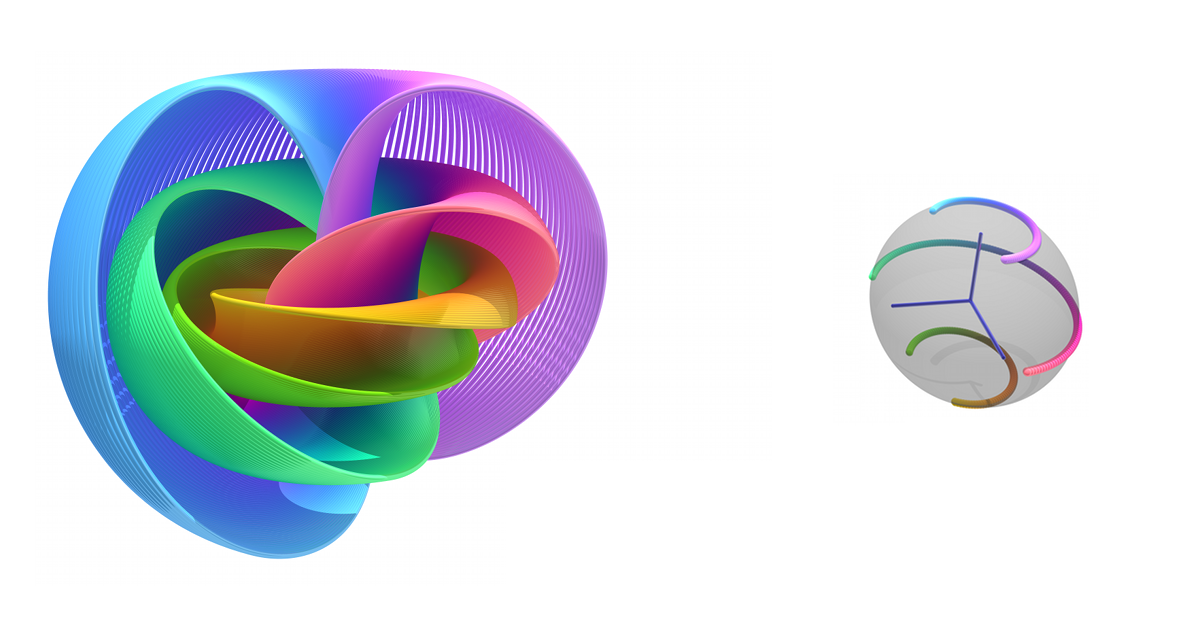
\includegraphics[width = 0.8\textwidth]{img/Hopf_Fibration.png}
\caption{Una representación de la fibración de Hopf, que lleva cada circunferencia de $\crc[3]$ a un punto en $\crc[2]$. Imagen vía \href{http://nilesjohnson.net/hopf.html}{Niles Johnson}, que tiene alguna animación chula sobre el tema.}
\label{fig:FibracionHopf}
\end{figure}

Para definir este fibrado trataremos de hacer algunas cuentas con la esfera $\crc[3]$. Sabemos que está dada por \[ \crc[3] = \set{ x,y,z,t ∈ ℝ \tq x^2 + y^2 + z^2 + t^2 = 1 } \]

La primera idea feliz es que la ecuación de arriba es equivalente a que $\abs{z}^2 + \abs{w}^2 = 1$ para $z,w ∈ ℂ$. Así, podemos meter la esfera dentro del plano completo: $\crc[3] ⊆ ℂ^2$.

La siguiente idea feliz es acordarnos de los espacios proyectivos de la \fref{sec:EspacioProyectivo}. Ahí definíamos $\projcp^1$, y de forma análoga a como teníamos en los reales (ver \fref{fig:EsferaPlanoProj}), en realidad no era más que la esfera con los puntos antipodales identificados. De la esfera podemos pasar a su proyección estereográfica, de tal forma que $\projcp^1 \cong ℂ ∪ \set{∞}$.

Con esto ya podemos definir nuestra proyección de $\crc[3]$ (tomada como subconjunto de $ℂ^2$) al espacio base del fibrado:
\begin{align*}
\appl{π}{\crc[3]&}{\projcp^1} \\
(z, w) &\longmapsto [z\cln w]
\end{align*}

El hecho clave de esta proyección es ver que dos puntos $(z,w), (z', w') ∈ ℂ^2$ tienen la misma imagen si existe un $λ ∈ ℂ$ tal que $z' = λz, w' = λw$, ya que en ese caso $[z\cln w]$ y $[z'\cln w']$ son la misma clase de equivalencia. Y ahora ya para la traca final, en ese caso y sabiendo que $\abs{z}^2 + \abs{w}^2 = \abs{z'}^2 + \abs{w'}^2 = 1$, tenemos que \[ 1 = \abs{z'}^2 + \abs{w'}^2  = \abs{λz}^2 + \abs{λw}^2 = \abs{λ}^2\left(\abs{z}^2 + \abs{w}^2 \right) = \abs{λ}^2 \] luego $\abs{λ} = 1$.

En otras palabras, lo que nos dice esto es que la proyección nos lleva todos los puntos de una misma circunferencia (multiplicar con un complejo de módulo 1 es simplemente rotar en una circunferencia) a un único punto en $\projcp^1$. Así, cada punto $[z\cln w] ∈ \projcp$ tiene asociada la fibra de puntos $e^{iθ}·(z,w)$ con $θ ∈ [0, 2π)$, que como decíamos es una cierta circunferencia. Para el resto de cuentas y una formalización algo mejor, es interesante leer \citep{liuHopfFibration} (que además habla de mecánica cuántica, que siempre mola).

Para nuestro caso de la geometría y topología, lo que nos faltaría ver es que efectivamente $\crc[3] \not\cong \crc[1] × \crc[2]$. Una demostración con cuentas sería totalmente infernal, pero sí que se podrá hacer con las cohomologías de De Rham que veremos en el \fref{chap:CohomologiaDeRham}.

\section{Campos vectoriales}

La definición de espacio tangente nos permite ampliar algo que ya se ve en cursos anteriores de cálculo, que son los campos vectoriales. Así, podremos definir campos en variedades arbitrarias que modelen cosas como el viento en una superficie o el campo magnético en el espacio.

\begin{defn}[Campo\IS vectorial] Un campo vectorial en $M$ es una aplicación \begin{align*}
\appl{X}{M&}{\tgs M = \bigcup \tgs_p M} \\
p &\longmapsto X(p) ∈ \tgs_p M
\end{align*}, donde $\tgs M$ es lo que se llama el \concept{Fibrado\IS tangente}.
\end{defn}

Esta es la definición general, aunque nosotros iremos directamente a por los que son diferenciables.

\begin{defn}[Campo\IS vectorial diferenciable] Un campo vectorial $X$ en $M$ se dirá diferenciable si localmente (esto es, en cada carta $(U, φ \equiv(x_1, \dotsc, x_m))$) es de la forma \[ X(p) = \sum_{i=1}^m λ_i(p) \eval{\dpd{}{x_i}}_p \] donde $λ_i ∈ C^∞(U)$. En realidad, la única cosa peculiar que pedimos es la diferenciabilidad de las $λ_i$, ya que siempre sabemos que un punto del tangente va a depender de esa base.
\end{defn}

Como siempre, el concepto no depende de la carta elegida.

\begin{example} Podemos dar un cambio en $\crc[2]$, a través de las dos cartas. Las definimos primero: \begin{gather*} U = \crc[2] \setminus \set{(0,0,-1)} \\
V = \set{ (x,y,t)  ∈ \crc[2] \tq t < 0}
\end{gather*} de tal forma que el campo puede ser \[ X(p) = \begin{cases}
\eval{\dpd{}{x_1}}_p & p ∈ U \\
\dfrac{1}{2} \left(-x^2 + y^2 + (1+t)^2\right) \eval{\dpd{}{y_1}}_p - xy \eval{\dpd{}{y_2}}_p & p ∈ V
\end{cases}\]

Desde luego, si $X$ es un campo tendrá que ser diferenciable. El problema es que no hemos comprobado si está bien definido, esto es, si ambas definiciones van a dar el mismo valor en los puntos de $U ∩ V$.

No pienso copiar las cuentas. El resultado es que sí, que está bien.
\end{example}

Sin entrar mucho en detalles (ver \citep[Capítulo VI]{ApuntesGeoDif} para algo mejor puesto), vamos a ver un ejemplo de la conexión de los campos vectoriales y la topología de una variedad.

\begin{theorem}[Teorema\IS de Poincaré-Hopf]Sea $X$ un campo definido en $M$. Entonces el número de ceros ``bien contados''\footnote{Es una enunciación del teorema muy vaga y poco formal, pero para enunciarlo bien hay que meterse en líos de índices de campos y no es plan.} coincide con la \nlref{def:CaracteristicaEuler} de la variedad $M$.\end{theorem}

Este es el teorema que permite demostrar otros como el ``teorema de la bola peluda'', que dice que, si le ponemos ``pelos'' a una pelota, nunca podremos peinarlos todos y siempre nos quedarán dos o más coronillas. Esa coronilla no es más que un cero del campo vectorial de pelos, y como la característica de Euler de la bola es 2, tiene que haber dos ceros ``bien contados''.

Igualmente, nos permite decir que el campo del ejemplo tiene que tener algún cero. De hecho, tendrá que anularse en el polo sur, cuando $t = -1$, y el índice de ese cero tendrá que ser 2.

\section{Espacio cotangente}

Una vez que tenemos definido el espacio tangente, vamos a querer hacer algo más que simplemente hablar de vectores tangentes. Querremos hablar de aplicaciones lineales sobre ellos, aplicaciones que por ejemplo nos puedan dar la longitud de un vector o, más tirando a nuestro campo de estudio, que nos permitan estudiar la topología a través de las formas diferenciales.

\begin{defn}[Espacio\IS cotangente] Dada una variedad $M$, se define el espacio cotangente a $M$ en $p ∈ M$ como el espacio dual de $\tgs_p M$, esto es, \[ \tgsd_p M = \mop{Hom}_ℝ (\tgs_p M, ℝ) = \set{\appl{A}{\tgs_p M}{ℝ} \tq A\text{ lineal, continua}} \]
\end{defn}

Por ser el dual, el cotangente tiene la misma dimensión que el tangente. Eso sí, el isomorfismo no es canónico\footnote{Esto es, que no hay una identificación canónica entre vectores del tangente y formas diferenciales como si pueda haber entre vectores de $ℝ^3$ y las aplicaciones lineales correspondientes.}. Si $(U, φ \equiv (x_1, \dotsc, x_m))$ es una carta alrededor de $p ∈ M$, entonces $\set{\eval[1]{\pd{}{x_i}}_p}_{i = 1, \dotsc, m}$ es una base de $\tgs_p M$. Nosotros denotaremos como $\set{\eval[1]{\dif x_i}_p}_{i=1,\dotsc, m}$ la base de $\tgsd_p M$ de tal forma que \[ \difp[x_i] \left(\eval{\dpd{}{x_j}}_p\right) = δ_{ij}\] donde $δ_{ij}$ es la \concept{Delta\IS de Kronecker}\footnote{$δ_{ij} = 1$ si $i = j$, $0$ en otro caso.}.

Como siempre, tendremos que tener cuidado con el cambio de coordenadas.

\textit{N.A.: A partir de ahora voy a pasar bastante de escribir dónde se evalúan los elementos de la base de los espacios tangentes, así que daré simplemente por supuesto que es en el punto $p$ y entonces $\eval{\dif x_i}_p = \dif x_i $, y $\eval[1]{\pd{}{x_i}}_p \equiv \pd{}{x_i}$. De hecho, por pura vaguería, diré que $\pd{}{x_i} \equiv ∂x_i$ tal que $\pd{f}{x_i} \equiv ∂x_i(f)$ y hala, todo bastante más sencillo.}

Si tenemos $(V, (y_1, \dotsc, y_m))$ otra carta, entonces podremos expresar \[ \dif x_i = \sum_{k=1}^m ∂y_k (x_i) · \dif y_k \]

La igualdad la probaremos aplicando a ambos lados $∂y_j$: \[ \dif x_i (∂y_j) =  \left(\sum_{k=1}^m ∂y_k (x_i) · \dif y_k \right)(∂y_j) = ∂y_j (x_i)\] y por otro lado \[ \dif x_i (∂y_j) = \dif x_i \left(\sum_{k=1}^m ∂y_j(x_k) · ∂x_k\right) = \sum_{k=1}^m ∂y_j(y_k) · \dif x_i (∂x_k) = ∂y_j(x_i) \], que efectivamente es lo mismo.

Con esto ya podemos definir lo que es un campo de covectores ó 1-forma diferencial.

\begin{defn}[Campo\IS de covectores] \label{def:CampoCovectores} Un campo de covectores ó 1-forma diferencial es una aplicación \begin{align*}
\appl{ω}{M&}{\bigcup \tgsd_p M = \tgsd M} \\
p &\longmapsto ω(p) ∈ \tgsd_p M
\end{align*}, donde $\tgsd M$ es lo que llamaremos el \concept{Fibrado\IS cotangente}.
\end{defn}

Un ejemplo sencillo es ver que, dada una aplicación $\appl{f}{M}{ℝ}$ con $f ∈ C^∞$, $\dif f$ es una forma diferencial. ¿Cómo podemos definir exactamente qué es la diferencial de una función? Antes hemos visto que $\dif x_i$ son los elementos de la base de $\tgsd_p M$. Intuitivamente, lo que podemos ver es que $\dif x_i (∂x_j) = δ_{ij}$ nos dice algo que en el fondo es bastante obvio: que la coordenada $x_i$ sólo varía cuando nos movemos en su misma dirección, y que si nos movemos la dirección de cualquier otra coordenada entonces $x_i$ no cambia.

Así, de forma análoga, lo que podemos ver es que $\dif f$ será una aplicación que nos diga cuánto varía $f$ cuando nos movemos en una cierta dirección $(v_1, \dotsc, v_m) = \vv ∈ \tgs_p M$. Si pensamos en el gradiente que vemos en cursos de cálculo, lo que hacemos en el fondo es multiplicar la coordenada $i$-ésima de la dirección en la que nos movemos (la dada por el vector $\vv ∈ \tgs_p M$) por la derivada parcial de $f$ con respecto a la $x_i$. En otras palabras, lo que debería ser $\dif f$ es algo como esto: \[ \dif f = \sum_{i=1}^m \pd{f}{x_i} · \dif x_i \], de tal forma que cuando lo quisiésemos aplicar a un vector $\vv = \sum v_i ·∂x_i$ nos quedaría \[ \dif f (\vv) = \sum_{i=1}^m \pd{f}{x_i} · \dif x_i (\vv) = \sum_{i=1}^m \pd{f}{x_i} · \dif x_i \left(\sum_{j=1}^m v_j · ∂x_j\right) = \sum_{i=1}^m \pd{f}{x_i} · v_i \], que es efectivamente lo que nos sale\footnote{Para el último salto, hemos usado que $\dif x_i$ es una aplicación lineal y que $\dif x_i (∂x_j) = δ_{ij}$.} si hubiésemos pensado en el gradiente de $f$.

\section{Formas diferenciales}

Cuando hemos definido el concepto de \nlref{def:CampoCovectores}, hemos dicho que también se podría llamar 1-forma diferencial. El nombre no es casualidad, así que vamos a ponernos a definir qué son las formas diferenciales y para qué sirven.


\subsection{Motivación}
\label{sec:MotivFormas}

¿Qué es una forma diferencial? Aquí la explicación de \citep{tao2007differential} es muy interesante, y haremos un pequeño resumen. Si recordamos las clases de física de Bachillerato, existían funciones de energía $F$ de tal forma que el trabajo para subir una masa unitaria de una altura $a$ a una altura $b$ era $\int_a^b F(x) \dif x$.

En los cursos de cálculo siempre se dice que $\dif x$ no es nada más que notación, y que nos indica con respecto a qué variable integrar. Pero podemos mirar todo ese integrando de forma conjunta, suponiendo, como hacían los matemáticos clásicos, que $\dif x$ es un ``incremento infinitesimal''. Así, $F(x) \dif x$ no es más que lo que nos cuesta desplazar la masa una distancia infinitesimal $\dif x$.

¿Cómo podemos generalizar esto a dimensiones superiores? ¿Qué pasa si en lugar de subir la altura del objeto lo movemos a lo largo de una curva arbitraria $γ ∈ ℝ^3$? Tendremos lo mismo, salvo que contando con más dimensiones: ya no nos bastará con decir sólo el potencial cuando nos movemos en la dirección $x$, también en las direcciones $y$ y $z$. Así, la función a integrar sería algo como $ω = F_x(x,y,z) \dif x + F_y(x,y,z) \dif y + F_z(x,y,z) \dif z$, que en cada punto nos dirá cuánto nos cuesta mover la masa en una dirección $\vv ∈ ℝ^3$. No es casualidad que eso sea también una forma diferencial, que de hecho podemos integrar y sacar que el trabajo total sería $\int_γ ω$.

El siguiente paso es ver qué ocurre si no queremos tratar con curvas, sino con superficies. Por ejemplo, queremos ver cuánta luz pasa a través de una superficie transparente $M$, donde la luminosidad en cada punto vendrá dada por una función $f(x,y)$, con $x,y$ coordenadas de $M$. Para calcularlo, haremos la misma aproximación de siempre con las integrales: dividiremos la superficie en pequeños rectángulos de lado $Δx$ y altura $Δy$ y multiplicaremos por el valor de luminosidad en ese rectángulo: $\int_M f \approx \sum f(x,y) Δx Δy$. La cuestión es que no tenemos claro que siempre vayamos a poder dividir en rectángulos: igual $x$ e $y$ no son coordenadas perpendiculares y $Δx·Δy$ no nos da el área. Por suerte, este problema es salvable: simplemente usamos los paralelogramos definidos por los vectores $(x_1, x_2), (y_1, y_2)$, que tienen área $\det \left|\begin{smallmatrix} x_1 & y_1 \\ x_2 & y_2 \end{smallmatrix}\right|$. Así, estaríamos integrando la forma diferencial $f \dif x ∧ \dif y$, aplicándola a vectores tangentes a $M$ que son los que definen los pequeños rectángulos sobre los que integramos.

Que la definición de ese área sea la misma (aunque menos genérica) que la que dábamos en \eqref{eq:ApplFormaMultAlt} no es casualidad, igual que tampoco lo es que el volumen de un paralelepípedo esté dado por el determinante de los tres vectores que lo definen.

En resumidas cuentas, lo que hace la forma diferencial es darnos una longitud, un área o un volumen en una variedad. Nos permitirán hacer cálculos independientemente de las coordenadas de la variedad y, sobre todo, nos revelarán ciertos aspectos sobre la topología de las variedades, que es lo que estudiaremos en esta asignatura.

\subsection{Definición de las formas diferenciales}

Una vez que al menos hemos intentado dar significado a las formas diferenciales (no sé con cuánto éxito) vamos a ver la definición formal de todo esto.

\begin{defn}[Forma\IS multilineal alternada de grado $d$] Una forma multilineal alternada de grado $d$ sobre un espacio vectorial $V$ es una aplicación \[ \appl{T}{\underbracket{V×\dotsb ×V}_{d\text{ copias}}}{ℝ} \] lineal en cada variable, y donde alternada significa que si se repite un vector argumento el resultado es cero o, equivalentemente, que si cambiamos de orden dos vectores entonces cambia de signo \[ T(\dotsc, v_i, \dotsc, v_j, \dotsc) = - T(\dotsc, v_j, \dotsc, v_i, \dotsc)\]
\end{defn}

En lo que nos interesa a nosotros, $V$ será el espacio tangente $\tgs_p M$. Además, el espacio de todas estas formas lo denotaremos\footnote{Creo que en \citep{ApuntesGeoDif} esto lo llamamos el álgebra pinchorial. Magnífico nombre.} como $\mop{Alt}^d (V)$. Dos ejemplos sencillos es ver que $\mop{Alt}^0 (V) = ℝ$, o que $\mop{Alt}^1(V) =V^*$.

Además, si $\dim V = n$, entonces $\dim \mop{Alt}^n = 1$, y una base es el determinante, esto es, \begin{align*} \appl{\det}{V × \dotsb × V&}{ℝ} \\
(v_1, \dotsc, v_n) &\longmapsto \det \begin{vmatrix} v_1^1 &  & v_n^1 \\ \vdots & \ddots & \vdots \\ v_1^n & & v_n^n \end{vmatrix}
\end{align*}

En general, podremos dar una base para el espacio de formas alternadas: a partir de una base $\set{e_i}_{i=1, \dotsc, n}$ de $V$, la base será la dada por covectores $\set{e_{i}^*}$\begin{align}
\appl{e_{i_1}^* ∧ \dotsb ∧ e_{i_d}^*}{\overbracket{V × \dotsb × V}^{d\text{ copias}}&}{ℝ} \nonumber \\
e_{i_1}^* ∧ \dotsb ∧ e_{i_d}^*(v_1, \dotsc, v_d) &= \det \begin{vmatrix}
e_{i_1}^* (v_1) & \cdots & e_{i_d}^* (v_1) \\
\vdots & \ddots & \vdots \\
e_{i_1}^* (v_d) & \cdots & e_{i_d}^* (v_d)
\end{vmatrix} \label{eq:ApplFormaMultAlt} \end{align} donde $e_i^* (e_j) = δ_{ij}$. En otras palabras, $e_{i}^*(v)$ extrae la coordenada $i$-ésima del vector $v$ o, equivalentemente, si $v = \sum v_i e_i$, entonces $e_i^* (v) = v_i$.

Vista la base algebraica, podemos ir a definir lo que es una forma diferencial.

\begin{defn}[Forma\IS diferencial] Dada $M$ una variedad diferenciable de dimensión $n$, una $k$-forma diferencial es una aplicación que a cada punto $p ∈ M$ le asigna una forma multilineal alternada de grado $k$ definida sobre el espacio $\tgs_pM$:
\begin{align*}
\appl{ω}{M&}{\mop{Alt}^k(\tgs_p M)} \\
p & \longmapsto ω(p)
\end{align*}

La forma lineal tiene como expresión local \[ ω = \sum_{i_1, \dotsc, i_k = 1}^n a_{i_1, \dotsc, i_k} (x_1, \dotsc, x_n) \dif x_{i_1} ∧ \dotsb ∧ \dif x_{i_k} \], donde $\dif x_i$ son los elementos de la base del dual $\tgsd_p M$. Tomando multíindices $I \equiv i_1, \dotsc i_k$, la definición se puede abreviar como $ω = \sum_{I} a_I \dif x_I$.
\end{defn}

De momento, lo de ``expresión local'' lo ignoraremos hasta que veamos el pullback. De momento, una 2-forma diferencial en $ℝ^3$ puede ser algo como $ω = (x + y + z) \dif x ∧ \dif z$. Esta forma la evaluaremos en un punto $p = (3,4,5)$, por ejemplo, y después la aplicaremos a dos vectores $\vv_1 = (-1,0,-2)$, $\vv_2 = (1,1,1)$ (con cuidado de hacerlo con el determinante como en \eqref{eq:ApplFormaMultAlt}). Si hacemos el cálculo, tenemos lo siguiente: \[
ω_p(\vv_1, \vv_2) = (3 + 4 + 5) · \det \begin{vmatrix} -1 & 1 \\ -2 & 1 \end{vmatrix} = 12 · 1 = 12 \]


\subsection{Operaciones con formas diferenciales}

Por abreviar, $Ω^k(M)$ será nuestro espacio de trabajo, el espacio vectorial de formas diferenciales de grado $k$ definidas sobre $M$. Si $ω ∈ Ω^k(M)$ entonces

Sabíamos que $Ω^0(M) = C^∞(M)$ y que además, localmente, podemos expresar las formas diferenciales como \[ \restr{ω}{U} = \sum a_{i_1, \dotsc, i_k} \dif x_1 \y \dotsb \y \dif x_k \] donde $\set{x_i}$ es un sistema de coordenadas del entorno $U$ y con $\set{\dif x_i}$ el dual de $\set{∂x_i}$. Con esta base, podemos empezar a definir las operaciones sobre formas diferenciales.

\subsubsection{Producto exterior}

La primera operación es el producto exterior, una aplicación $\appl{∧}{\Omega^r(M)×\Omega^s(M)}{\Omega^{r+s}(M)}$ compatible con las cartas, que definiremos de la siguiente forma.

\begin{defn}[Producto\IS exterior] Dadas una $m$-forma $ω = \sum a_I \dif x_I$ y otra $n$-forma $τ = \sum b_J \dif x_J$ con $I,J$ multiíndices, su producto exterior es una $(m+n)$-forma que se define como \[ ω ∧ τ = \sum_{I,J} a_I b_J \dif x_I ∧ \dif x_J \], teniendo en cuenta que $\dif x_i ∧ \dif x_i = 0$.
\end{defn}


\subsubsection{Diferencial exterior}

La diferencial es una aplicación lineal \begin{align*}
\appl{\dif}{Ω^k(\bola^n)&}{Ω^{k+1}(\bola^n)} \\
ω = h \dfl{t_{i_1}}{t_{i_n}} &\longmapsto \dif ω = \dif h ∧ \dfl{x_{i_1}}{x_{i_n}}
\end{align*}

Sólo damos la definición para un término porque es lineal. Por ser un poco más concretos, \[ \dif ω = \sum_{j=1}^k \left(\dpd{h}{x_j} \dif x_j \right) \dfl{x_{i_1}}{x_{i_n}} \]

La diferencial tiene una serie de propiedades:

\begin{prop} \label{prop:PropsDiferencial} Propiedades de la diferencial exterior:
\begin{enumerate}
\item $\dif (ω ∧ η) = \dif ω ∧ η + (-1)^{\deg ω} ω ∧ \dif η $.
\item \label{prp:DifDifCero} $\dif (\dif ω) = 0$.
\item \label{prp:CompatDifPullback} Dada $\appl{f}{ℝ^m}{ℝ^n}$, entonces $f^* (\dif ω) = \dif(f^*ω)$.
\end{enumerate}
\end{prop}

\begin{proof}

\proofpart{$\dif (ω ∧ η) = \dif ω ∧ η + (-1)^{\deg ω} ω ∧ \dif η $}

Tomamos $ω = \sum f_I \dif x_I$, $η = \sum g_J \dif x_J$, con $I,J$ multiíndices. Entonces operamos: \begin{align*}
\dif (ω ∧ η) &= \dif \left(\sum_{I,J} (f_I · g_J) \dif x_I ∧ \dif x_J \right)
	= \sum_{I,J} \dif(f_I · g_J) \dif x_I ∧ \dif x_J = \\
	&= \sum_{I,J} \left(\sum_{k = 1}^N \dpd{(f_I · g_J)}{x_k} \right) \dif x_k ∧ \dif x_I ∧ \dif x_J = \\
	&= \sum_{I,J} \left(\sum_{k = 1}^N g_J \dpd{f_I}{x_k} + f_I \dpd{g_J}{x_k}\right) \dif x_k ∧ \dif x_I ∧ \dif x_J = \\
	&= \sum_{I,J} \sum_{k=1}^N \left(\dpd{f_I}{x_k} \dif x_k ∧ \dif x_I ∧ (g_J \dif x_J) + \dpd{g_J}{x_k} \dif x_k ∧ (f_I \dif x_I) ∧ \dif x_J \right) = \\
	&= \sum_{I,J} \left(\sum_{k=1}^N \dpd{f_I}{x_k} \dif x_k ∧ \dif x_I ∧ (g_J \dif x_J)\right) + \\ & \qquad + \sum_{I,J} \left(\sum_{k=1}^N \dpd{g_I}{x_k} \dif x_k ∧ (f_I \dif x_I) ∧ \dif x_J \right) = \\
	&= \sum_{I,J} \left(\sum_{k=1}^N \dpd{f_I}{x_k} \dif x_k ∧ \dif x_I ∧ (g_J \dif x_J)\right) + \\ & \qquad + \sum_{I,J} \left(\sum_{k=1}^N (-1)^{\deg ω} \dpd{g_I}{x_k} \dif x_k ∧ \dif x_J ∧ (f_I \dif x_I) \right) = \\
	&= \dif ω ∧ η + (-1)^{\deg ω} ω ∧ \dif η
\end{align*}, donde el $(-1)^{\deg ω}$ aparece al mover $\deg ω$ diferenciales (las del multiíndice $\dif x_I$) para ordenarlo todo bien.

\proofpart{$\dif(\dif ω) = 0$}

\end{proof}

Con esto podemos definir bien la diferencial en una variedad abstracta.

\begin{defn}[Diferencial\IS exterior] Dada una forma diferencial $ω ∈ Ω^k(M)$, entonces definimos la diferencial como \begin{align*}
\appl{\dif}{Ω^k(M)&}{Ω^{k+1} (M)} \\
ω &\longmapsto \dif ω = \sum_{j=1}^k \left(\dpd{h}{x_j} \dif x_j \right) \dfl{x_{i_1}}{x_{i_n}}
\end{align*}

Y declaramos que esto es perfectamente compatible con las cartas, es decir, que si $(φ_U ○ \inv{φ_V})^* ω_U = ω_V$, entonces $(φ_U ○ \inv{φ_V})^* \dif ω_U = \dif ω_V$. Sólo hay que usar la \fref{prp:CompatDifPullback}.
\end{defn}

\subsubsection{Pullback}

Dada una aplicación $\appl{F}{M}{N}$, queremos ver cómo podemos llevar formas diferenciales de $N$ a formas diferenciales en $M$.

\begin{defn}[Pullback] Dada una aplicación $\appl{f}{M}{N}$ entre variedades diferenciables, el pullback nos lleva formas diferenciales de $N$ a $M$ y está dado por \begin{align*}
	\appl{F^*}{Ω^k(N)&}{Ω^k(M)} \\
	ω &\longmapsto f^* ω
\end{align*} donde
\begin{align*}
	\appl{(F^*ω)(p)}{\tgs_p M × \dotsb × \tgs_p M&}{ℝ} \\
	(v_1, \dotsc, v_k) &\longmapsto ω(F(p)) \left(\difp(v_1), \dotsc, \difp (v_k) \right)
\end{align*}
donde $\difp$ es la \nlref{def:DiferencialAplicacion}. \end{defn}

Para ver cómo funciona el pullback, vamos a ver un ejemplo para
\[
	\appl{f}{ℝ^m}{ℝ^n}
\]
, con $f(x) = (f_1(x), \dotsc, f_n(x))$ y coordenadas $(x_1, \dotsc, x_m)$ para $ℝ^m$ e $(y_1, \dotsc, y_n)$ para $ℝ^n$.
Entonces, dada una forma diferencial $\dif x_j ∈ Ω^1(ℝ^m)$ entonces \[ f^*(\dif y_j) = \sum_{k=1}^m \pd{f_j}{x_k} \dif x_k = \dif f_j \]

Para comprobarlo, lo que hacemos es un chorro de cuentas aplicando eso a vectores tangentes $∂y_j$ y sale.

Ahora nos podemos hacer una pregunta para hacer cuentas todavía más infernales: ¿qué ocurre si cogemos una $2$-forma $\dif y_i ∧ \dif y_j ∈ Ω^2(ℝ^n)$? Bueno, pues lo que sale es que
\[
	f^* (\dif y_i ∧ \dif y_j)
	= \sum_{k,l=1}^n \dpd{f_i}{x_k} \dpd{f_j}{x_k} \dif x_k ∧ \dif x_l
\], y de nuevo si lo aplicamos a dos vectores, tenemos que
\[
	\left(\sum_{k,l=1}^n \dpd{f_i}{x_k} \dpd{f_j}{x_k} \dif x_k ∧ \dif x_l\right)(∂x_r, ∂x_s)
	= \pd{f_i}{x_r} \pd{f_k}{x_s}
\] por la definición de base dual ($\dif x_i (∂x_j) = δ_{ij}$). Por el otro lado,
\begin{align*}
\left(f^*(\dif y_i ∧ \dif y_j)\right) (∂x_r, ∂x_s)
	&= \dif y_i ∧ \dif y_j\left(\Dif f (∂x_r), \Dif (∂x_s)\right) = \\
	&= \dif y_i ∧ \dif y_j
		\left(
			\sum_{α=1}^m \dpd{f_α}{x_r} ∂y_α,
			\sum_{β=1}^m \dpd{f_β}{x_s} ∂y_β,
		\right) = \\
	&= \dpd{f_i}{x_r} \dpd{f_j}{x_s}
\end{align*}

Efectivamente, tenemos lo mismo y por lo tanto el pullback es compatible con el producto exterior.

\subsubsection{Resumen}

Dado el caos que son las secciones anteriores, ponemos un pequeño resumen de las operaciones y sus propiedades. En general, tenemos $ω = \sum a_I \dif x_I$ de grado $m$ y $τ = \sum b_J \dif x_J$ de grado $n$.

\paragraph{Producto exterior}
\begin{align*}
ω ∧ τ &= \sum a_I b_J · \dif x_I ∧ \dif x_J \\
\dif x_i ∧ \dif x_i &= 0
\end{align*}

\paragraph{Diferencial exterior} \begin{align*}
\dif ω &= \sum_{I} \left(\sum_{i} \dpd{a_I}{x_i} \dif x_i \right) \dif x_I \\
\dif(\dif ω) &= 0 \\
\dif(ω+τ) &= \dif ω + \dif τ \\
\dif(ω ∧ τ) &= \dif ω - τ + (-1)^k ω ∧ \dif τ
\end{align*}

\paragraph{Pullback} Dada $\appl{f}{M}{N}$, con $f(x_1, \dotsc, x_m) = (f_1, f_2, \dotsc, f_n)$ entonces \begin{align*}
f^*ω &= \sum_{I} f ○ a_I · \dif f_I = \sum_{I} a_I(f(x_1, \dotsc, x_m)) \bigwedge_{i ∈ I} \left(\sum_{j=1}^n \dpd{f_i}{x_j} \dif x_j \right) \\
f^*(\dif ω) &= \dif (f^*ω) \\
f^*(ω∧τ) &= f^*ω ∧ f^*τ \\
f^*(ω+τ) &= f^*ω + f^*τ
\end{align*}

\subsection{Expresión local de formas diferenciales}

Hasta ahora hemos dejado de lado el tema de las cartas, y no hemos comprobado si todas las operaciones y las formas diferenciales son compatibles con las cartas. Pero eso tenemos que comprobarlo: queremos ver si, dado un punto $p$ y dos cartas $U, V$ para un entorno de $p$, las formas diferenciales definidas en esas cartas coinciden.

\begin{figure}[tbhp]
\inputtikz{CartasFormasDiferenciales}
\caption{Aquí pondría el dibujo para ver qué es exactamente lo que tenemos que demostrar, pero como no tengo ni idea de qué es lo que tengo que hacer pues lo dejo así.}
\label{fig:CartasFormas}
\end{figure}


\begin{prop} $ω(p)$ no depende de la carta elegida para $p$.
\end{prop}


%%%% CLase copiada por dejuan.
\[
	\Omega(M) = \bigoplus_{k≥0} \Omega^K(M)
\]
Es el espacio de todas las formas diferenciales y es un espacio vectorial.


Sea $ω$ una forma diferencial de grado $d$. Entonces,

\[
	ω \equiv \left\{
			ω_u\in\Omega_+^d(φ(u))\\
				+
			ω_v = (φ_uφ_v^{-1})^\ast ω_u
	\right\}_{u\in \text{atlas}}
\]

De esta manera, podemos escribirlo en términos de funciones, tomando $I$ como multiíndice, con lo que $\dif x_I = \dif x_{i1}\wedge \dotsb  \wedge \dif x_{in}$

\[ω_u = \sum_{|I| =d}a_I^u \dif x_I\]


\begin{example}
Vamos a ver un ejemplo con la \concept{forma angular}, $i^*ω = dθ$, la función $\appl{i}{S^1}{\real^2}$ y $ω = -y\dif x + x \dif y$.

Tenemos
\[
	\dif θ \equiv \left\{ \begin{array}{c} \dif θ\in Ω^1(0,2π)\\\dif θ\in Ω^1(-π,π)\end{array}\right.
\]

Las funciones transición $φ_1$ y $φ_2$ son las funciones transición tales que $\appl{φ_1}{e^{iθ}}{θ}$ en $(0,2π)$ y  $\appl{φ_2}{e^{iθ}}{θ}$ en $(-π,π)$.


Ahora nos planteamos si es cierto $i^*ω\left( \dpa{}{θ}\right)_{|p_0} = 1$, tomando $p_0 = e^{iθ_0}$

\begin{align*}
	&i^*ω\left( \dpa{}{θ}\right)_{|p_0} = ω\left(\dif i \left( \dpa{}{θ}\right) \right) = \\
	&ω\left(
			\dpa{x·i}{θ}_{|_{θ_0}} \dpa{}{x}_{|_{p_0}}
	\right)  =
	ω\left(
		-\sin θ_0 \dpa{}{x}_{|_p} + \cos θ_0 \dpa{}{y}_{|_{p_0}}
	\right)\\
	&= -y\dif x + x\dif y \left(
		-\sin θ_0 \dpa{}{x}_{|_p} + \cos θ_0 \dpa{}{y}_{|_{p_0}}
	\right) \\
	&= ... = -\sin(θ_0)(-\sin θ_0)·1 + \cos(θ_0)\cos(θ_0) = 1
\end{align*}

¿Y cuánto valdría $i^*(\dif x ∧ \dif y)$? Necesariamente es $0$, ya que en $S^1$ no caben formas diferenciales mayores de la dimensión. Es decir:

\[
	\Omega(M) = \bigoplus_{k≥0}^{∞} \Omega^K(M) = \bigoplus_{k≥0}^{\dim{M}} \Omega^K(M)
\]

\end{example}

\chapter{Cohomología de De Rham}
\label{chap:CohomologiaDeRham}

Una vez vista toda la base de variedades diferenciables y formas diferenciables, vamos a ir al núcleo de este curso: la cohomología de De Rham.

¿Qué es la cohomología y por qué es interesante? Si recordamos los cursos de topología\footnote{Si no los recordamos, ver \citep[Capítulo III]{ApuntesTopologia}.}, había algo llamado el ``grupo fundamental'', que lo que hacía era darnos una idea de cómo estaba conectado un conjunto según pudiésemos deformar unos caminos cerrados en otros.

Un problema de ese grupo fundamental es que es algo difícil de estudiar, así que se toma un enfoque alternativo. Sabemos que el grupo fundamental nos puede dar el número de componentes conexas por caminos. Resulta que esa información también nos la puede dar las funciones que son localmente constantes: si tenemos una componente conexa sólo podemos coger funciones de la forma $f = k$ con $k ∈ ℝ$, luego tenemos dimensión 1. Pero si tenemos dos componentes conexas, podemos coger un valor constante para la primera y otro valor para la segunda componente: tenemos un espacio de funciones de dimensión 2.

La ventaja de este enfoque es que es muy fácil de computar: las funciones constantes son las que tienen diferencial nula. Luego, dada nuestra variedad $M$, podremos definir \[ H^0(M) = \set{\appl{f}{M}{ℝ} \tq \dif f = 0} \] como el grupo de cohomología de dimensión 0, cuya dimensión nos da el número de componentes conexas de una variedad.

La ventaja además de esa definición es que lo podemos extender sin mucho problema a dimensiones superiores, simplemente pidiendo que $\dif ω = 0$ (las formas que cumplen $\dif ω = 0$ son las \concept{Formas\IS cerradas}) Por supuesto, ya sabemos que $\dif (\dif η) = 0$ luego querremos quitarnos las que vienen como diferencial de otra forma diferenciasl (\concept{Formas\IS exactas}). Así, podemos llegar al grupo de cohomología:

\begin{defn}[Grupo\IS de cohomología] Se define el grupo $k$-ésimo de cohomología de De Rham como \[ H^k (M) = \quot{\ker \dif ^k}{\img \dif^{k-1}} \] cuya dimensión es $h^k(M) = \dim H^k(M)$, donde definimos la aplicación $\dif^k$ como la diferencial exterior de formas de grado $k$: $\appl{\dif^k}{Ω^k(M)}{Ω^{k+1}(M)}$.
\end{defn}

¿Cómo podemos interpretar ese grupo de cohomología? La primera forma es recordar el \concept{Teorema\IS de Stokes}, que dice que para una variedad diferenciable orientable, se tiene \( \int_{∂Ω} ω = \int_Ω \dif ω  = 0 \qquad (ω ∈ \ker \dif^k ) \label{eq:StokesRham} \)

Dado que nosotros estamos estudiando la cohomología de la variedad $M$, asumiremos que $∂Ω ⊂ M$. Si suponemos $ω ≠ 0$ (no sería demasiado interesante) podemos buscar qué nos hace falta para que $ω ∉ \img \dif^{k-1}$. Lo hacemos por reducción al absurdo: suponemos que $\dif η = ω$ y aplicamos Stokes de nuevo. Como $∂Ω$ ya es el borde de una variedad, su borde es vacío, luego \[ 0 = \int_{∅} η = \int_{∂Ω} ω \]

Si lográsemos demostrar que $\int_{∂Ω} ω ≠ 0$ entonces tendríamos directamente que esa forma η no existe y que ω no es exacta. Por supuesto, esto entra en bastante contradicción con lo que hemos visto en \eqref{eq:StokesRham}, así que algo tiene que fallar.

Una posibilidad es que $γ = ∂Ω$ no sea el borde de ninguna variedad (recordamos que tiene que ser una subvariedad de $M$) y que tenga $∂γ = ∅$. La otra posibilidad es que aunque $∂Ω$ sí sea el borde de una variedad, no podamos aplicar en ella Stokes (por ejemplo, si le falta un punto en el interior).

\begin{figure}[hbtp]
\centering
\inputtikz{FallosStokes}
\caption{Stokes puede fallar en dos casos: o bien estamos integrando a lo largo de un camino que no encierra nada (por ejemplo, la curva γ que rodea el interior del toro) o bien estamos integrando en un borde de una variedad en la que no se puede aplicar Stokes (por ejemplo, si le falta un punto del interior).}
\label{fig:FallosStokes}
\end{figure}

En cualquiera de los dos casos tenemos el mismo tipo de información: agujeros. La cohomología de De Rham nos dice qué formas diferenciales nos están gritando que han encontrado un agujero en la variedad. En este caso, el ejemplo lo hemos hecho con formas de grado 1 (las estamos integrando a lo largo de líneas) pero la analogía vale para más dimensiones.

Un ejemplo rápido es calcular la cohomología de $ℝ$, que sale \( H^k(ℝ) \cong \begin{cases} ℝ & k = 0 \\ \set{0} & k = 1 \\ \set{0} & k > 1 \end{cases} \label{eq:CohomologiaR} \)

En cuanto nos pasamos de la dimensión de $ℝ$, el grupo de cohomología es $\set{0}$ (no hay formas diferenciales de grado mayor que la dimensión de la variedad). Para formas de grado $k = 0$, tenemos que el grupo es de dimensión $1$ porque sólo hay una componente conexa.

El único punto a verificar sería el de $k = 1$, pero eso sale fácil: \[ H^1(ℝ) = \quot{\ker \dif^1}{\img \dif^0} = \quot{\set{ω = f(t) \dif t}}{\set{η = \dif φ, φ ∈ C^∞(ℝ)}} = \set{0} \] ya que ambos espacios son iguales: $ω = f(t) \dif t = \dif φ$ con $φ = \int_0^t f(s) \dif s$.

Aunque en general no lo usaremos demasiado, se le puede dar una estructura algebraica a la cohomología de De Rham.

\begin{defn}[Anillo\IS de cohomología] \label{def:AnilloCohomologia} Dada $M$ una variedad diferenciable, se define su anillo de cohomología como la suma directa\footnote{Para nosotros, la suma directa es lo mismo que el producto cartesiano. \href{http://math.stackexchange.com/questions/39895/the-direct-sum-oplus-versus-the-cartesian-product-times}{Hay algunas diferencias sutiles cuando tratamos con sumas infinitas}.} de cada grupo de cohomología \[ H^*(M) = \bigoplus_{k ≥ 0} H^k(M) \]

$H^*(M)$ es un anillo con las operaciones $+$, $∧$.
\end{defn}

Habría que comprobar para ver que es un anillo que si $ω, η$ son cerradas entonces $ω ∧ η$ y $ω + η$ son cerradas, y que además esto no depende de la elección del representante\footnote{Como lo que estudiamos son formas cerradas, sabemos que $[ω] = [ω + \dif ω_1]$}. Son un montón de cuentas sin ninguna dificultad que salen directamente.

\section{Resultados básicos}

Antes de ver herramientas más fuertes para tratar la cohomología de De Rham, vamos a ver algunos resultados básicos y más sencillos sobre lo que ocurre en cohomologías de variedades que son difeomorfas o que son homótopas. Dado que antes veíamos que la cohomología nos dice algo sobre la topología de las variedades, lo que esperamos es que las cohomologías sean iguales si la transformación no nos cambia la topología de la variedad.

\subsection{Invarianza por homeomorfismos}

\begin{prop} \label{prop:CohomDifeomorfismo} Sean $N$, $M$ dos variedades diferenciables y sea $\appl{f}{M}{N}$ un difeomorfismo entre ellas. Entonces, los grupos de cohomología son isomorfos ($H^k(N) \cong H^k(M)$).

Además, $f$ induce isomorfismos de espacios vectoriales y de anillos respectivamente  \begin{align*}
\appl{f^*}{H^k(N)&}{H^k(M)} \\
\appl{f^*}{H^*(N)&}{H^*(M)}
\end{align*}
\end{prop}

\begin{proof} Para la demostración basta ver que el pullback $f^*$ lleva formas cerradas en formas cerradas y formas exactas en formas exactas.

Es fácil ver que, dada $ω ∈ Ω^k(N)$, entonces se cumplen ambas cosas:\begin{align*}
ω \text{ cerrada}: \dif ω = 0 &\implies \dif (f^* ω) = f^* (\dif ω) = 0 & f^* ω\text{ cerrada}\\
ω \text{ exacta}: ω = \dif η &\implies f^* ω = f^*(\dif η) = \dif (f^* η) & f^* ω \text{ exacta}
\end{align*}

Igualmente podemos considerar el pullback inverso $\inv{f^*} = (\inv{f})^*$ que está bien definido por ser $f$ difeomorfismo, y tendremos el isomorfismo.
\end{proof}

\subsection{Invarianza por homotopías}

Pasará algo parecido con dos variedades homótopas, aunque la demostración llega un poco más de trabajo (tampoco mucho).

\begin{theorem} Supongamos que $\appl{f,g}{M}{N}$ son aplicaciones homótopas. Entonces $f^* = g^*$ a nivel de cohomología.
\end{theorem}

\begin{wrapfigure}{R}{0.4\textwidth}
\inputtikz{FuncionMeseta}
\caption{Una función ``meseta'' $α ∈ C^∞$ que varía suavemente de $0$ a $1$ en el intervalo $[0,1]$.}
\label{fig:FuncionMeseta}
\end{wrapfigure}

\begin{proof}
Consideramos la aplicación \begin{align*}
\appl{F}{[0,1] × M&}{N} \\
(t,x) &\longmapsto F_t(x)
\end{align*} donde $F_0 = f$ y $F_1 = g$.

Por otra parte, sea $\appl{α}{ℝ}{[0,1]}$ una función meseta como en la \fref{fig:FuncionMeseta}. Entonces definimos \begin{align*}
\appl{G}{M×ℝ&}{N} \\
(x,t) & \longmapsto F(α(t), x)
\end{align*} y tal que \begin{align*}
(G○s_0) (x) &= G(x,0) = F(0,x) = F_0(x) = f \\
(G○s_1) (x) &= G(x,1) = F(1,x) = F_1(x) = g
\end{align*}

Entonces $f^* = (G○s_0)^* = s_0^* ○ G^* = s_1^* ○ G^* = (G○s_1)^* = g^*$ y listos, así que a nivel cohomológico son iguales.
\end{proof}

Con esto ya podemos ir a demostrar que dos variedades homótopas son iguales.

\begin{corol} \label{crl:CohomHomotopia}
Si dos variedades $M, N$ son homótopas entonces sus anillos de cohomología son iguales.
\end{corol}

\begin{proof} [Vía \href{http://math.stackexchange.com/questions/1196461/why-is-de-rham-cohomology-invariant-under-deformation-retraction-or-more-gener}{Math.SX}] Dado que $M, N$ son homótopas entonces podemos definir dos aplicaciones $\appl{f}{M}{N}$ y $\appl{g}{N}{M}$ tales que $f ○ g \simeq g ○ f \simeq \mop{Id}$ (esto es, cuya composición es homotópicamente equivalente a la identidad).

El teorema anterior nos dice que entonces $\mop{Id}^* \simeq (g ○ f)^* = f^* ○ g^*$ y análogamente para $(f ○ g)^*$. Finalmente, tenemos que $\appl{f^*}{H^k(N)}{H^k(M)}$ y $\appl{g^*}{H^k(M)}{H^k(N)}$ son aplicaciones con inversas bien definidas, luego son biyectivas y por lo tanto inducen un isomorfismo entre $H^k(M)$ y $H^k(N)$.
\end{proof}

Una aplicación de esto es ver que $\crc[1]$ no es un retracto por deformación de $ℝ^2$. Si lo fuera, los grupos de cohomología serían ambos nulos $H^1(ℝ^2) = 0$ pero $-y\dif x + x \dif y ∈ H^1(\crc[1])$ no es exacta.

En general, podemos ver que $H^k(ℝ^{n+1} \setminus \set{0}) \cong H^k(\crc[n])$. ¿Cómo encontrar un generador de $H^1(ℝ^2 \setminus \set{0})$. Bueno, podemos coger la contracción $r(x) = \frac{x}{\norm{x}}$ y entonces la forma generadora es \[ r^*(\dif θ) = r^*\left(\frac{-y \dif x + x \dif y}{x^2 + y^2}\right) \]

\subsection{Cohomología de $M × ℝ$. Lema de Poincaré}
\label{sec:LemaPoincare}

Por último, vamos a ver un resultado que luego ampliaremos, que es ver qué ocurre con el producto cartesiano de una variedad con $ℝ$.

\begin{prop} \label{prop:CohomMR} Sea $M$ una variedad diferenciable. Entonces $H^k(M × ℝ) = H^k(M)$.
\end{prop}

\begin{proof} La idea es la misma que la de la demostración del \fref{crl:CohomHomotopia}: dar una composición que sea la identidad a nivel de homotopía de tal forma que cada una de las funciones sea biyectiva.

En este caso, definimos la proyección y el ``levantamiento'' de la siguiente forma:
\begin{align*}
M × ℝ &\longmapsto M \\
(x, k)&\xrightarrow{\; π \;} x \\
(x, k)& \xleftarrow{\; s_k \;} x
\end{align*}

Es obvio que $π ○ s_k = \mop{Id}$ y que por lo tanto $s_k^* ○ π^* = \mop{Id}^*$. En el otro sentido no es así ($s_k ○ π ≠ \mop{Id}$), aunque a nivel de homotopía se puede demostrar que existe un cierto operador que nos hace que $π^* ○ s_k^* = \mop{Id}^*$ y ya tendríamos todo bien. Ahora bien, la demostración es algo larga y no la voy a copiar. Al que le interese, que lea \citep[Sec. 4]{bott2013differential}.
\end{proof}

Trivialmente, este resultado nos da la cohomología de $ℝ^n$ a partir de la de $ℝ$ que ya habíamos visto en \eqref{eq:CohomologiaR}: \( H^k(ℝ^n) = \begin{cases} ℝ & k = 0 \\ \set{0} & k ≠ 0 \end{cases} \label{eq:CohomologiaRN} \)

Además, esto sirve para dar una demostración muy rápida del Lema de Poincaré.

\begin{lemma}[Lema\IS de Poincaré] \label{lem:Poincare} Sea $M$ una variedad contractible. Entonces toda forma cerrada es exacta.

Equivalentemente, \( H^k(\bola^n) = \begin{cases} ℝ & k = 0 \\ \set{0} & k ≠ 0 \end{cases} \label{eq:CohomologiaBN} \)
\end{lemma}

\begin{proof} Una variedad contractible (en particular, $\bola^n$ es contractible) es difeomorfa a $\bola^n$, luego según la \fref{prop:CohomDifeomorfismo} su cohomología es isomorfa a la de $ℝ^n$, que ya la habíamos visto en \eqref{eq:CohomologiaRN}.
\end{proof}

\section{Cálculo de cohomologías: Mayer-Vietoris}

Hasta ahora hemos visto algunos resultados para calcular cohomologías. Sabemos que si $M$ es conexa, entonces $H^0(M) = 0$, que $H^k(\bola^n) = 0$ cuando $k > 0$ por el \nref{lem:Poincare}, y que además si $M_1 \simeq M_2$ (homotópicamente equivalentes) entonces $H^*(M_1) = H^*(M_2)$ (\fref{crl:CohomHomotopia}).

Sin embargo, para otros cálculos de cohomologías no tenemos herramientas. Mayer-Vietoris será lo que usaremos para sacar cohomologías, trabajando con abiertos que cubren la variedad y estudiando su intersección. Para definirlo, primero necesitaremos una cierta base previa.

\begin{defn}[Sucesión\IS exacta de espacios vectoriales] Una sucesión exacta de espacios vectoriales es una cadena \[ \dotsb \to V_{i-1} \xrightarrow{h_{i-1}} V_{i} \xrightarrow{h_i} V_{i+1} \to \dotsb \] tales que $\ker h_i = \img h_{i-1}$.
\end{defn}

Por ejemplo, si tenemos una sucesión exacta \[ 0 \xrightarrow{h_0} V_1 \xrightarrow{h_1} V_2 \xrightarrow{
h_2} V_3 \xrightarrow{h_3} 0 \] podemos ver varias cosas, como que  $h_1$ es inyectiva ($\ker h_1 = \img h_0 = 0$) y que $h_3$ es suprayectiva ($\ker h_3 = \img h_2 = V_3$). Entrando en temas menos obvios, podemos aplicar el primer teorema de isomorfía para $h_2$, de tal forma que \[ \quot{V_2}{V_1} \cong V_3 \]

En ejemplos más concretos, podemos definir una cadena exacta \[ 0 \to ℝ^2 \overset{h_1}{\hookrightarrow} ℝ^5 \xrightarrow{h_2} ℝ^3 \mapsto 0 \], con \begin{align*}
h_1(x_1, x_2) &= (x_1, x_2, 0,0,0) \\
h_2(y_1, y_2, y_3, y_4, y_5) &= (y_3, y_4, y_5)
\end{align*} donde en la última aplicación tenemos que mandar los elementos de $\img h_1$ a $0$ si queremos que sea exacta.

Volviendo a las formas diferenciales, podemos volver a la cadena \[0 \to Ω^0(\bola^n) \xrightarrow{\dif^0} Ω^1(\bola^n) \xrightarrow{\dif^2} \dotsb \xrightarrow{\dif^{k-1}} Ω^{k}(\bola^n) \xrightarrow{\dif^k} Ω^{k+1}(\bola^n)\], que será una sucesión exacta si y sólo si $\ker \dif^{i+1} = \img \dif^i$, equivalente a decir que $\quot{\ker \dif^{i+1}}{\img \dif^i} = H^{i+1}(\bola^n) = 0$. Es un resultado interesante porque nos permite vincular el resultado algebraico (que la cadena sea exacta o no) a un resultado sobre cohomologías.

\begin{prop} Si la cadena \[ 0 \to V_0 \xrightarrow{h_0} V_1 \to \dotsb \to V_{n-1} \xrightarrow{h_{n-1}} V_{n} \to 0 \] es exacta, entonces la suma alternada de dimensiones de los espacios vectoriales es cero:  \[ \sum_{i=0}^n (-1)^i \dim V_i = 0\]
\end{prop}

\begin{proof}
\label{prop:sumaAlternada0}
Podemos considerar las dos siguientes cadenas: \begin{align*}
0 \to \img h_1 & \xhookrightarrow{i} V_1 \to \dotsb \to V_{n-1} \xrightarrow{h_{n-1}} V_{n} \to 0 \\
0 \to V_0 &\xrightarrow{h_0} V_1 \xrightarrow{h_1} \img h_1 \to 0
\end{align*}, que son sucesiones exactas, y entonces podemos razonar por inducción sumando las formulitas de la suma de dimensión, aunque personalmente no tengo del todo claro por qué está usando lo que quiere probar para demostrarlo exactamente lo mismo.
\end{proof}

\begin{theorem}[Sucesión\IS exacta de Mayer-Vietoris] \label{thm:SucesionMayerVietoris} Sean $U,V$ abiertos de $M$ tales que $M = U ∪ V$. Entonces la siguiente sucesión es exacta:

\begin{center}
\tikzexternaldisable
\begin{tikzcd}[row sep = 3pt, column sep = 8pt]
0 \rar & Ω^*(M) \arrow{r}{r} & Ω^*(U) \oplus Ω^*(V) \arrow{r}{\delta} & Ω^* (U ∩ V) \rar & 0 \\
	& ω \arrow{r}{r}	& (\left.ω\right|_U, \left.ω\right|_V) & & \\
	&  & (η_1, η_2) \arrow{r}{\delta} & \left.η_2\right|_{U∩V} - \left.η_1\right|_{U∩V} &
\end{tikzcd}
\tikzexternalenable
\end{center}
\end{theorem}

\begin{proof} $r$ es inyectiva porque $U ∪ V = M$, y además $\ker δ ⊇ \img r$ obviamente: \[ δ○r (ω) = δ(\restr{ω}{U}, \restr{ω}{V}) = \restr{ω}{U∩V} - \restr{ω}{U∩V} = 0 \]

Por otra parte, si $(η_1, η_2) ∈ \ker δ$, entonces $\restr{η_2}{U∩V} = \restr{η_1}{U∩V}$. Entonces, definimos \[ η = \begin{cases} η_1 & \text{en } U \\ η_2 & \text{en } V \end{cases} \], y entonces está claro que está bien definida (en la intersección ambas coinciden, y $U ∪ V = M$) y $r(η) = (η_1, η_2)$.

Nos falta ver que $δ$ es suprayectiva. Sea $σ ∈ Ω(U∩V)$. Necesitamos encontrar $η_1 ∈ Ω(U)$, $η_2 ∈ Ω(V)$ tal que $σ = \restr{η_2}{U∩V} - \restr{η_1}{U∩V} $. Así, definimos una partición de la unidad de $M$ subordinada al recubrimiento de $M$ formado por $U$ y $V$, esto es, dos aplicaciones $\appl{ρ_{U,V}}{M}{ℝ^+}$, con $\sop ρ_U ⊂ U$, $\sop ρ_V ⊂ V$ y además $ρ_U + ρ_V = 1$.

Con esto en la mano, lo que tenemos que definir (o eso le parece a Gabino al menos) es \begin{align*}
η_1 &= -ρ_V σ ∈ Ω(U)\\
η_2 &= ρ_U σ ∈ Ω(V)
\end{align*} salvo signo, y con las formas valiendo $0$ fuera de $U ∩ V$.

Si suponemos que esta definición es buena, entonces haciendo las restricciones correspondientes a $U∩V$ $η_2 - η_1 = ρ_Uσ + ρ_Vσ = σ$, booooooom shakalaka.
\end{proof}

Un ejemplo de esa partición para $\crc[n]$, con dos funciones concretas. que cumplen efectivamente lo que se pedía, con $\tilde{ρ}_U = ρ ○ φ_U$ en $\crc[n] \setminus{S}$ y $0$ en otro caso donde $φ_U$ es la carta y $ρ$ algo. Entonces se pueden definir \[ ρ_U ≝ \frac{\tilde{ρ}_U}{\tilde{ρ}_U + \tilde{ρ}_V} \qquad ρ_V ≝ \frac{\tilde{ρ}_V}{\tilde{ρ}_U + \tilde{ρ}_V} \], de tal forma que el soporte es el que necesitamos y ya está.

\begin{theorem}[Teorema\IS de Mayer-Vietoris de cohomología] \label{thm:MayerVietoris} La siguiente sucesión es exacta
\[ \dotsb \xrightarrow{\dif^*} H^{k-1} (U∩V) \xrightarrow{\dif^*} H^k(M) \xrightarrow{r} H^k(U) \oplus H^k(V) \xrightarrow{δ} H^k(U∩V) \xrightarrow{\dif^*} H^{k+1} (M)  \xrightarrow{\dif^*} \dotsb \]

$r$, y $δ$ definidas como en el \fref{thm:SucesionMayerVietoris}, y $\dif^*$ es más difícil de definir (Gabino dixit).
\end{theorem}

\subsection{Aplicación: Cohomología de $\crc[n]$}

\begin{figure}[hbtp]
\centering
\inputtikz{S1Cover}
\caption{Un atlas de $\crc[1]$ con dos abiertos $U, V$ y su intersección para calcular Mayer-Vietoris.}
\label{fig:S1Cover}
\end{figure}

La primera aplicación de esto es poder calcular la cohomología de $\crc[1]$ con las cartas $U,V$ de toda la vida (\fref{fig:S1Cover}). La idea es que $H^0(U) \oplus H^0(V)$ tiene dimensión 2, $H^0(U∩V)$ tiene dimensión dos por ser dos componentes conexas, $\dim H^1(U) = \dim H^1(V) = 0$ por ser $U,V$ homeomorfos a $ℝ$ y entonces hay una sucesión metida entre dos ceros. Como la suma alternada de dimensiones es cero, tenemos que \[ 1 - 2 + 2 - \dim H^1(M) + 0 = 0\] y por lo tanto $\dim H^1(\crc[1]) = 1$.

Así, al final tenemos que \( H^k(\crc[1]) = \begin{cases} ℝ & k = 0,1 \\ \set{0} & k > 1 \end{cases} \label{eq:CohomologiaS1} \)

\begin{figure}[hbtp]
\centering
\inputtikz{CoverS2}
\caption{Cobertura de $\crc[2]$ con dos abiertos $U,V$, que podemos considerar como $\crc[2]$ menos el polo sur y norte respectivamente.}
\label{fig:S2Cover}
\end{figure}

Este resultado se puede ampliar a la esfera ($\crc[2]$) usando un argumento parecido. Lo que hacemos es tomar una cobertura con dos abiertos $U,V$ quitando el polo sur y norte respectivamente, como en la \fref{fig:S2Cover}. Cada uno de ellos es homeomorfo a $\bola^2$, y su intersección (una banda alrededor de la esfera) es homótopa a $\crc[1]$.

La cadena de Mayer-Vietoris que nos queda es la siguiente:
\begin{center}
\tikzexternaldisable
\begin{tikzcd}[row sep = 3pt]
0 \rar
	& H^0(\crc[2]) \rar & H^0(U) \oplus H^0(V) \rar & H^0(U ∩ V) \arrow[snake]{dll}{} \\
	& H^1(\crc[2]) \rar & \textcolor{red!70!black}{H^1(U) \oplus H^1(V)} \rar & H^1(U ∩ V) \arrow[snake]{dll}{} \\
	& H^2(\crc[2]) \rar & \textcolor{blue!70!black}{H^2(U) \oplus H^2(V)} \rar & H^2(U ∩ V) \rar & 0 \\
\end{tikzcd}
\tikzexternalenable
\end{center}

Tenemos una ventaja, que es que $H^1(U) \oplus H^1(V) = H^2(U) \oplus H^2(V) = \set{0}$ así que podemos dividir la cadena en dos subcabenas que siguen siendo exactas. Para la primera tenemos los siguientes espacios con sus respectivas dimensiones:
\begin{center}
\tikzexternaldisable
\begin{tikzcd}[row sep = 0pt, column sep = 7pt]
0 \rar
	& H^0(\crc[2]) \rar & H^0(U) \oplus H^0(V) \rar & H^0(U ∩ V) \rar &  H^1(\crc[2]) \rar & \textcolor{red!70!black}{H^1(U) \oplus H^1(V)}\\
	& 1 & 1 \oplus 1 = 2 & 1 & ? & 0
\end{tikzcd}
\tikzexternalenable
\end{center}

La única dificultad en esta cadena está en ver que $U ∩ V \simeq \crc[1]$ y por lo tanto $H^0(U ∩ V) = H^0(\crc[1]) = ℝ$, porque el resto es el número de componentes conexas y ver que la dimensión de la suma directa es la suma de las dimensiones. Así, simplemente despejamos en la suma alternada:
\begin{align*}
0 &= 1 - 2 + 1 - \dim H^1(\crc[2]) \\
0 &= \dim H^1(\crc[2]) ≝ h^1(\crc[2])
\end{align*}

Es decir, $\dim H^1(\crc[2]) = 0$ (recordemos la notación $\dim H^k(M) ≝ h^k(M)$, que es más cómoda).

Vamos ahora con la otra cadena, que igualmente sale sencilla:
\begin{center}
\tikzexternaldisable
\begin{tikzcd}[row sep = 0pt, column sep = 7pt]
\textcolor{red!70!black}{H^1(U) \oplus H^1(V)} \rar
	& H^1(U ∩ V) \rar & H^2(U ∩ V) \rar & H^2(\crc[2]) \rar & \textcolor{blue!70!black}{H^2(U) \oplus H^2(V)}\\
0 & 1 & 0 \oplus 0 = 0 & ? & 0
\end{tikzcd}
\tikzexternalenable
\end{center}

El truco en esta está de nuevo en ver que $U ∩ V \simeq \crc[1]$, y ya habíamos calculado $H^1(\crc[1])$ en \eqref{eq:CohomologiaS1}. Así, es fácil ver que $h^2(\crc[2]) = 1$. Juntando todo, podemos sacar la cohomología de la esfera: \( h^k(\crc[2]) = \begin{cases} 1 & k = 0 \\ 0 & k = 1 \\ 1 & k = 2 \end{cases} \label{eq:CohomologiaS2} \)

Podríamos ampliar este resultado (ver \fref{ej:Hoja7:CohomologiaSN} para más detalles) y nos saldría algo parecido para esferas $n$-dimensionales: sólo tenemos dimensión cuando $k = 0$ o cuando $k = n$ \(
h^k(\crc[n]) = \begin{cases}
1 & k = 0 \\
0 & k ≠ 0,n \\
1 & k = n\end{cases} \label{eq:CohomologiaSN} \)

En el fondo, esto concuerda con la idea intuitiva que le habíamos dado a la cohomología: que nos revela agujeros. En el caso de la esfera $n$-dimensional no hay agujeros hasta que no llegamos a la dimensión de la esfera entera, donde el ``agujero'' es el que ella misma encierra.

\section{Dualidad de Poincaré}

Una herramienta adicional para poder calcular las homologías es la dualidad de Poincaré, que nos dice cuál es el espacio vectorial dual de un espacio de cohomología de una variedad de dimensión $n$. Para ello, construiremos el producto de dualidad a través de la integral y tendremos es la siguiente relación: \[ H^q(M) \cong \dual[H_c^{n-q}(M)]\] donde $H_c^{n-q}$ es la cohomología de formas con soporte compacto (necesitaremos esto para garantizarnos integrales finitas). Además, necesitaremos pedir que $M$ sea orientable y comprobar que las cohomologías tienen dimensión finita (si no, el tratamiento de los duales es bastante más delicado).

\subsection{Cohomologías de soporte compacto}

A la hora de estudiar el espacio dual, parece claro que si queremos asignar un número real a una forma diferencial lo que tendremos que hacer será integrar. Ahora bien, podemos tener problemas si la variedad no es compacta: la integral se puede ir a infinito.

Para evitarnos ese problema, desarrollaremos las cohomologías de soporte compacto, en las que nos restringiremos a formas diferenciales de soporte compacto y que por lo tanto tendrán una integral finita. Por recordar, el soporte de una forma es \[ \sop ω = \set{ p ∈ M \tq ω_p ≠ 0} \]

\begin{defn}[Grupo\IS de cohomología de soporte compacto] Sea $M$ una variedad diferenciable. Se define $Ω_c^k(M)$ como las $k$-formas diferenciales de soporte compacto. Consideramos entonces la diferencial $\appl{\dif_c^k}{Ω_c^k(M)}{Ω_c^{k+1}(M)}$, y definimos el grupo de cohomología de soporte compacto como \[ H_c^k(M) = \quot{\ker \dif_c^k}{\img \dif^{k-1}_c} \]
\end{defn}

Obviamente, $H_c^k(M) = H^k(M)$ cuando $M$ es una variedad compacta.

Aquí nos gustaría reproducir el resultado de la \fref{sec:LemaPoincare} y del \fref{prop:CohomMR}, que nos decía que $H^k(M×ℝ) \cong H^k(M)$. Pero hay un problema, y es que aquí el pullback de la proyección $\appl{π}{M×ℝ}{M}$ no tiene por que llevar una forma de soporte compacto en $Ω_c(M)$ a una forma de soporte compacto en $Ω_c(M × ℝ)$. Por suerte, ocurre al revés. Tendremos el siguiente lema (que no vamos a demostrar):

\begin{prop} \label{prop:CohomCompMR} Sea $M$ una variedad diferenciable. Entonces \[ H_c^k(M) \cong H_c^{k+1}(M×ℝ)\]
\end{prop}

Esto nos lleva directamente al Lema de Poincaré para formas con soporte compacto.

\begin{lemma}[Lema\IS de Poincaré para soportes compactos] \label{lem:PoincareCompactos} \( H_c^k(ℝ^n) = \begin{cases} ℝ & k = n \\ 0 & k ≠ n\end{cases} \label{eq:CohomologiaCompRN} \)
\end{lemma}

\begin{proof}

Procederemos por inducción, viendo que se cumple para $n = 1$ y haciendo inducción cuando $n ≥ 2$.

\proofpart{$n = 1$}

Es fácil ver que $H_c^0(ℝ) = \set{0}$: la única función constante de soporte compacto en $ℝ$ es la función constante $0$. Cualquier otra tiene como soporte todo $ℝ$, que no es compacto.

Vamos a ver ahora que $H^1(ℝ) \simeq ℝ$. Toda forma $ω ∈ Ω_c^1(ℝ)$ se puede escribir como $ω = g(x) \dif x$, con $\appl{g}{ℝ}{ℝ}$ de soporte compacto. Así, podemos decir que $ω = \dif f$ con \begin{align*}
\appl{f}{ℝ&}{ℝ} \\
x & \longmapsto \int_{-∞}^x g(t) \dif t
\end{align*}

Para que $ω$ sea exacta, necesitaremos que $f ∈ Ω_c^0(ℝ)$, esto es, que tenga soporte compacto y por lo tanto que la integral de $g(t)$ se anule.

Equivalentemente, si definimos la aplicación lineal \begin{align*}
\appl{φ}{Ω_c^1(ℝ)&}{ℝ} \\
ω &\longmapsto \int_{ℝ} ω
\end{align*} lo que tenemos es que $\ker φ = \img \dif^0$.

Aquí nos vamos ahora al álgebra. El primer teorema de isomorfía nos dice que $\quot{Ω_c^1(ℝ)}{\ker φ} \cong \img φ$. Sólo nos faltan dos piezas: que $φ$ es sobreyectiva, luego $\img φ = ℝ$, y que $\ker \dif^1 = Ω_c^1(ℝ)$, ya que estamos en $ℝ$, de dimensión $1$, y ahí toda $1$-forma es cerrada. Juntándolo todo: \[ H^1(ℝ) = \quot{\ker \dif^1}{\img \dif^0} = \quot{Ω_c^1(ℝ)}{\ker φ} \cong \img φ = ℝ \]

\proofpart{$n ≥ 2$}

Aplicando la \fref{prop:CohomCompMR} con $M = ℝ^{n-1}$, tenemos que $H_c^{k - 1}(ℝ^{n-1}) \cong H_c^k(ℝ^n)$. Cuando $k = n$ podemos ir por inducción y llegar a que $H_c^n(ℝ^n) \cong H_c^1(ℝ) \cong ℝ$.

Cuando $k = 0$, lo que tenemos es que $H_c^0(ℝ^n) = \set{0}$ por el mismo argumento que cuando $n = 1$: la única función constante de soporte compacto en $ℝ^n$ es $f = 0$.

Finalmente, cuando $0 < k < n$ hacemos inducción de nuevo con la \fref{prop:CohomCompMR} y llegaremos a que $H_c^k(ℝ^n) \cong H_c^0(ℝ^{n-k}) \cong \set{0}$.
\end{proof}

La sucesión de Mayer-Vietoris también es válida aquí, aunque justo al revés.

\begin{prop} \label{prop:MayerVietorisCompacto} Sea $M$ una variedad diferenciable y $U,V$ dos abiertos tales que $U ∪ V = M$. Entonces la siguiente sucesión es exacta:

\begin{center}
\tikzexternaldisable
\begin{tikzcd}[row sep = 3pt]
0 & Ω^*(M) \arrow{l}{} & Ω^*(U) \oplus Ω^*(V) \arrow{l}{r} & Ω^* (U ∩ V) \arrow{l}{\delta} & \arrow{l}{} 0
\end{tikzcd}
\tikzexternalenable
\end{center}
\end{prop}

\begin{proof}
La única dificultad está en definir bien las aplicaciones. Lo primero que hacemos es definir la inclusión $\appl{i_*}{Ω_c^k(U)}{Ω_c^k(M)}$. Dado $U ⊂ M$ y $ω ∈ Ω_c^k(U)$, la extendemos con cero a una forma $\tilde{ω} ∈ Ω_c^k(M)$ de la siguiente forma: \[ \tilde{ω}_p = \begin{cases} ω_p & p ∈ U \\ 0 & p ∉ U \end{cases} \]

Así, definimos la inclusión con signo \begin{align*}
\appl{δ}{Ω^*_c(U∩V)&}{Ω_c^*(U) \oplus Ω_c^*(V)} \\
ω &\longmapsto (i_* ω, i_* ω)
\end{align*} con $i_*$ la inclusión de $U ∩V$ en $U$ y $V$ respectivamente.

La otra aplicación que falta es la suma, donde simplemente llevamos una forma $(η_1, η_2)$ a la suma $η_1 + η_2 ∈ Ω_c^*(M)$.
\end{proof}

Esta secuencia da lugar de nuevo a una secuencia a nivel de cohomologías para una variedad $M$ de dimensión $n$:

\begin{center}
\tikzexternaldisable
\begin{tikzcd}[row sep = 3pt]
0 	& H^0(M) \arrow{l}{} & \arrow{l}{} H^0(U) \oplus H^0(V) & \arrow{l}{} H^0(U ∩ V)  \\
	& \phantom{H^0(M)} \arrow[snake up]{urr}{} & \dotsb & \phantom{H^1(U ∩ V)} \\
	& H^n(M) \arrow[snake up]{urr}{} & \arrow{l}{} H^n(U) \oplus H^n(V) & \arrow{l}{} H^n(U ∩ V) & \arrow{l}{} 0 \\
\end{tikzcd}
\tikzexternalenable
\end{center}

\subsection{Dimensión finita de la cohomología de De Rham}

Para facilitarnos los cálculos, necesitaremos ver que las cohomologías siempre tienen dimensión finita, de tal forma que podamos manejar el dual sin problemas. Para ello, introducimos la noción de ``buen recubrimiento''.

\begin{defn}[Buen\IS recubrimiento] \label{def:BuenRecubrimiento}
Se dice que $U_1,U_2,\dotsc,U_n$, con $U_i$ contractibles, es un buen recubrimiento para una variedad diferenciable $M$ si $\bigcup U_i = M$ y si la intersección $U_i ∩ U_j$ es o bien vacía o bien un abierto contractible.
\end{defn}

En particular, es importante porque toda variedad tiene un buen recubrimiento. No haremos la prueba porque no es difícil pero requiere meterse en temas de geometría Riemanniana.

\begin{theorem} Sea $M$ una variedad diferenciable. Entonces, existe un buen recubrimiento. Si además $M$ es compacta, el recubrimiento puede escogerse finito.
\end{theorem}

Esto nos lleva a la siguiente proposición, bastante sencillita:

\begin{prop}\label{prop:CohomologiaFinita} Sea $M$ una variedad diferenciable con un buen recubrimiento. Entonces su cohomología tiene dimensión finita.
\end{prop}

\begin{proof} Aplicando Mayer-Vietoris, la cohomología de cada abierto es fácil de sacar y por lo tanto tenemos dimensiones finitas por todas partes.
\end{proof}

\subsection{Construcción de la dualidad de Poincaré}

Recapitulemos un poco. La dualidad de Poincaré pretende demostrar el siguiente isomorfismo: \[ H^q(M) \cong \dual[H_c^{n-q}(M)]\]

Para ello, lo que hacemos es dar un emparejamiento que nos permita construir el dual de un grupo de cohomología. Para eso, necesitamos dar una aplicación bilineal que nos diga como construir una aplicación lineal sobre formas en $H_c^{n-q}(M)$ a partir de formas en $H^q(M)$. La forma de definir el emparejamiento será a través de la integral, y aquí es donde necesitamos lo que hemos visto antes de cohomología de soporte compacto: queremos evitar que la integral se vaya a infinito.

Además, si no queremos volvernos locos con el dual, necesitaremos que todos los grupos de cohomología sean finitos. Si no, hay ciertas suposiciones que no podemos hacer (por ejemplo, que un espacio vectorial sea isomorfo a su dual).

Una vez recapitulado todo esto, vamos a por el plato fuerte.

\begin{theorem}[Dualidad\IS de Poincaré] \label{lem:DualidadPoincare} Sea $M^n$ una variedad diferenciable orientable con un \nlref{def:BuenRecubrimiento}. Entonces, la aplicación lineal \begin{align*}
\appl{\pesc{·,·}}{H^p(M) × H^{n-p}_c(M)&}{ℝ} \\
(ω,η) &\longmapsto \int_M ω ∧ η
\end{align*} es bilineal y no degenerada (esto es, si $\pesc{ω, η} = 0$ para todo $η$ entonces $ω = 0$).
\end{theorem}

La definición del emparejamiento nos dice por qué le pedimos a la variedad que sea orientable: si no lo fuese, una $n$-forma podría anularse\footnote{Ver \citep[Def. IV.7]{ApuntesGeoDif}: una variedad $M^n$ es orientable si y sólo si existe una $n$-forma $ω$ en $M$ tal que $ω_p ≠ 0$ para todo $p ∈ M$.}.

Para la demostración necesitaremos el siguiente lema.

\begin{lemma}[Lema\IS de los cinco] \label{lem:delos5} Consideramos el siguiente diagrama conmutativo con dos cadenas exactas de grupos abelianos.

\begin{center}
\tikzexternaldisable
\begin{tikzcd}
\dotsb \rar
	& A \arrow{r}{f_1} \arrow{d}{\alpha}
	& B \arrow{r}{f_2} \arrow{d}{\beta}
	& C \arrow{r}{f_3} \arrow[red!80!black]{d}{\gamma}
	& D \arrow{r}{f_4} \arrow{d}{\delta}
	& E \arrow{r}{} \arrow{d}{\epsilon}
	& \dotsb \\
\dotsb \rar
	& A' \arrow{r}{f_1'}
	& B' \arrow{r}{f_2'}
	& C' \arrow{r}{f_3'}
	& D' \arrow{r}{f_4'}
	& E' \rar
	& \dotsb
\end{tikzcd}
\tikzexternalenable
\end{center}

Si los homomorfismos $α,β,δ,ε$ son isomorfismos, entonces $γ$ también es isomorfismo.
\end{lemma}

\begin{proof}[\nref{lem:delos5}]
\href{https://es.wikipedia.org/wiki/Lema_de_los_cinco}{Para consultar la demostración.}
\end{proof}

\begin{proof}[\nref{lem:DualidadPoincare}]

La demostración se hace por inducción sobre el número $k$ de abiertos de un ``buen recubrimiento''.

\proofpart{$k = 1$}

Si $M$ se puede recubrir con un único abierto contractible, entonces $M \simeq ℝ^n$. En ese caso, gracias a los lemas de Poincaré para cohomología normal (\fref{lem:Poincare}) y para cohomología con soporte compacto (\fref{lem:PoincareCompactos}) sabemos calcular las cohomologías:
\[
H_c^p(ℝ^n) = \begin{cases} ℝ & p = n \\ 0 & p ≠ n\end{cases}
\qquad
H^p(ℝ^n) = \begin{cases} ℝ & p = 0 \\ \set{0} & p ≠ 0 \end{cases}
\]

Dado que estamos con cohomologías finitas (\fref{prop:CohomologiaFinita}), tenemos que $H_c^p(ℝ^n) \cong \dual[H_c^p(ℝ^n)]$ así que ya lo tenemos: \[  H^p(M) \cong H^p(ℝ^n) \cong H_c^{n-p}(ℝ^n) \cong \dual[H_c^{n-p}(ℝ^n)] \cong \dual[H_c^p(M)] \]

\proofpart{Inducción: $k \to k + 1$}

Vamos a aplicar Mayer-Vietoris de la siguiente manera, tomando abiertos $U,V$ a partir del recubrimiento con $k + 1$ abiertos: \[
	M = \underbracket{U_1 \cup \dotsb \cup U_k}_{U} \cup \underbracket{U_{k+1}}_{V}
\]

Por hipótesis de inducción, tenemos que $U, V$ tienen buenos recubrimientos con $k$ y 1 abiertos respectivamente.

Además, $U\cap V = (U_1\cap U_{n+1})\cup \dotsb \cup (U_n\cap U_{n+1})$, y por construcción y definición de los buenos recubrimientos, este es un buen recubrimiento con $k$ abiertos.

Ahora ya estamos en condiciones de aplicar Mayer-Vietoris para $p$ (\fref{thm:MayerVietoris}) y Mayer-Vietoris para compactos (\fref{prop:MayerVietorisCompacto}) del complementario ($q = n - p$).

\begin{center}
\tikzexternaldisable
\begin{tikzcd}[column sep = 8pt]
  H^p(U) \oplus H^p(V) \arrow{r}{} \arrow[green!70!black, leftrightarrow]{d}
& H^p(U ∩ V) \arrow{r}{} \arrow[green!70!black, leftrightarrow]{d}
& H^p(M) \arrow{r}{} \arrow[red!80!black, leftrightarrow]{d}
& H^{p+1}(U) \oplus H^{p+1}(V) \arrow{r}{} \arrow[green!70!black, leftrightarrow]{d}{}
& H^{p+1}(U ∩ V) \arrow[green!70!black, leftrightarrow]{d}{}
	\\
  H_c^{q}(U) \oplus H_c^{q}(V)
& H_c^{q}(U ∩ V) \arrow{l}{}
& H_c^{q}(M) \arrow{l}{}
& H^{q-1}_c(U) \oplus H^{q-1}_c(V) \arrow{l}{}
& H^{q-1}_c(U ∩ V) \arrow{l}{}
\end{tikzcd}
\tikzexternalenable
\end{center}

Las flechas verdes corresponden a isomorfismos por hipótesis de inducción. $V$ tiene 1 abierto y $U$ tiene $k$ abiertos, con lo que los correspondientes son isomorfos. Hemos construido este diagrama para poder aplicar el \nref{lem:delos5} y concluir que la aplicación representada por la flecha roja es un isomorfismo. Dado que además $H_c^q(M)$ es isomorfo a su dual, entonces lo que tenemos es que
\[ H_c^{n-p}(M) \cong H^p(M) \] con lo que tenemos demostrado el teorema.
\end{proof}

\section{Cohomología de variedades producto: Teorema de Künneth}

En la \fref{sec:LemaPoincare} habíamos resuelto un caso específico de la cohomología de la variedad producto, cuando hacíamos $M × ℝ$. Ahora bien, nos gustaría saber qué ocurre con el producto de una variedad producto más general, de tal forma que podamos estudiar fibrados y saber si son no triviales (por ejemplo, cuando estudiamos la \nlref{sec:FibracionHopf}, nos dejamos pendiente el ver que $\crc[1] \not\cong \crc[1] × \crc[2]$ para comprobar que el fibrado no era trivial). La solución a este caso nos la da el Teorema de Künneth:


\begin{theorem}[Teorema\IS de Künneth] \label{thm:Kunneth} Sean $M$, $N$ dos variedades diferenciables y $\appl{π_1, π_2}{M×N}{M,N}$ las respectivas proyecciones naturales. Entonces hay un isomorfismo \[ \bigoplus_{p+ q = d} H^p(M) \otimes H^q(N) \cong H^d (M × N)\] donde se asocian formas diferenciales de la siguiente forma \[ (ω^p \otimes η^q)_{p+q = d} \mapsto \sum_{p+q = d} π_1^* ω^p ∧ π_2^* η^q \]

A nivel de dimensiones, esto nos dice que
\[h^n(M×N) = \sum_{p+k=n} h^p(M)h^k(N)\]
\end{theorem}

Aunque no manejaremos mucho el producto tensorial, vamos a definirlo bien y explicarlo para poder entender exactamente lo que dice el teorema.

\begin{wrapfigure}[5]{R}[0.1\textwidth]{0.3\textwidth}
\centering
\vspace{-20pt}
\begin{tikzpicture}[yscale = 1.5, xscale = 2]
\node (VxW) at (0,0) {$V×W$};
\node (VoW) at (0, -1) {$V \otimes W$};
\node (E) at (1, 0) {$E$};

\draw[->] (VxW) -- node[midway, above] {$φ$} (E);
\draw[->] (VoW) -- node[midway, right] {$Φ$} (E);
\draw[->] (VxW) -- node[midway, left] {$\otimes$} (VoW);
\end{tikzpicture}
\vspace{-10pt}
\caption{Diagrama conmutativo para el producto tensorial.}
\label{fig:ProdTensorial}
\end{wrapfigure}

\begin{defn}[Producto\IS tensorial] Sean $V,W$ espacios vectoriales de dimensiones respectivas $n = \dim V$ y $m = \dim W$. Entonces existe un espacio vectorial $T = V \otimes W$ de dimensión $n m$ tal que existe una aplicación bilineal
\begin{align*}
	\appl{\otimes}{V×W&}{T} \\
	(v,w) &\longmapsto v \otimes w
\end{align*}

Además, para toda aplicación bilineal $\appl{φ}{V×W}{E}$ con $E$ otro espacio vectorial arbitrario existe una aplicación lineal $\appl{Φ}{T}{E}$ tal que el diagrama \ref{fig:ProdTensorial} es conmutativo (\concept{Propiedad\IS universal del producto tensorial}).

La construcción de los elementos del producto tensorial se hace de la siguiente forma. Dadas $\set{v_i}_{i=1}^n$ y $\set{w_j}_{j=1}^m$ bases respectivas de $V$ y $W$, entonces el producto tensorial lleva vectores de la siguiente forma: \begin{align*}
\appl{\otimes}{V×W&}{T} \\
\left(\sum a_i v_i, \sum b_j w_j\right) &\longmapsto \sum a_i b_j (v_i \otimes w_j)
\end{align*} donde los $(v_i \otimes w_j)$ serán los elementos de la base de $T$, de donde se deduce que la dimensión de $T$ es $n · m$.

Por otra parte, la aplicación Φ que hace conmutar el diagrama de la \fref{fig:ProdTensorial} se define a partir de los elementos de la base, como $Φ(v_i \otimes w_j) = φ(v_i, w_j)$.
\end{defn}

\begin{example} Algunos ejemplos de productos tensoriales:
\begin{itemize}
\item $V \otimes \set{0} = \set{0}$.
\item $V \otimes \kbb \cong \kbb$, donde $\kbb$ es el cuerpo base de $V$.
\item El ejemplo más interesante para nosotros. Dada la aplicación bilineal \begin{align*}
\appl{φ}{H^p(M) × H^q(N)&}{H^{p+q}(V × W)} \\
(ω, η) &\longmapsto π_1^* ω ∧ π_2^* η
\end{align*} existe, por la propiedad universal, una aplicación $Φ$ que hace conmutar el diagrama de la siguiente forma: \begin{align*}
\appl{Φ}{H^p(M) \otimes H^q(N)&}{H^{p+q}(V×W)} \\
ω \otimes η &\longmapsto π_1^* ω ∧ π_2^* η
\end{align*}
\end{itemize}
\end{example}


\begin{proof}[\nref{thm:Kunneth}, idea] Al igual que hemos hecho con otras demostraciones, se hará inducción sobre $k$, el número de abiertos de un buen cubrimiento de $N$.

Si $k$ fuese 1, entonces $N \cong \bola^n$, y por el \nref{lem:Poincare} tendríamos que $H^d(M × N) \simeq H^d(M)$, y en el otro lado $\bigoplus_{p+ q = d} H^p(M) \otimes H^q(N)$ se iría para todos los grupos de $N$ salvo cuando $q = 0$, luego la identificacíon saldría trivial.

% Me estoy quedando MUY dormido.
Para aplicar la hipótesis de inducción coge una sucesión exacta y lo multiplica tensorialmente por $H^p(M)$, de tal forma que sigue dando una sucesión exacta, y luego hace una suma directa en $p+q=d$ y al final pues debe haber un pifostio muy, muy importante que ni siquiera Edu ha copiado, por lo que yo no me siento obligado a hacerlo. Me voy a dejar la marquita de TODO para en algún momento antes del examen repasar esto de alguna fuente más fiable y o bien dejar la demostración bien hecha (aunque la hubiese copiado seguiría siendo una basura) o bien borrarlo.
\end{proof}

\subsection{Aplicación: la fibración de Hopf no es trivial}

Vamos a ver lo que teníamos pendiente de la \fref{sec:FibracionHopf}. Ahí habíamos demostrado que tenemos un fibrado local para $\crc[3]$ de tal forma que todo entorno $U ⊂ \crc[3]$ era isomorfo a $\crc[1] × \crc[2]$. Decíamos que era un fibrado no trivial porque aunque localmente ocurría eso, luego teníamos que $\crc[3] \not\cong \crc[1] × \crc[2]$ aunque no llegamos a demostrarlo.

Ahora sí que vamos a poder hacerlo usando la fórmula de Künneth.
\begin{align*}
	h^0(\crc[1]×\crc[2]) &= h^0(\crc[1])·h^0(\crc[2]) = 1\\
	h^1(\crc[1]×\crc[2]) &= h^0(\crc[1])h^1(\crc[2]) + h^0(\crc[1])h^1(\crc[2]) = 0 + 1 = 1\\
	h^2(\crc[1]×\crc[2]) &= h^0(\crc[1])h^2(\crc[2]) + h^1(\crc[1])h^1(\crc[2]) + h^2(\crc[1])h^0(\crc[2]) =  1+0+0 = 1\\
	h^3(\crc[1]×\crc[2]) &= h^0(\crc[1])h^3(\crc[2]) + h^1(\crc[1])h^2(\crc[2]) + h^2(\crc[1])h^1(\crc[2]) + h^3(\crc[1])h^0(\crc[2]) = 1
\end{align*}

Ahora bien, ya habíamos visto en \eqref{eq:CohomologiaSN} que \[
h^k(\crc[n]) = \begin{cases}
1 & k = 0 \\
0 & k ≠ 0,n \\
1 & k = n\end{cases} \], luego los grupos de cohomología no tienen la misma dimensión y por lo tanto $\crc[3] \not\cong \crc[1] × \crc[2]$.

Ya de paso vemos que se confirma la \nref{lem:DualidadPoincare}: tenemos que $h^0(\crc[1]×\crc[2]) = h^3(\crc[1]×\crc[2])$ y que $h^1(\crc[1]×\crc[2]) = h^2(\crc[1]×\crc[2])$.


\section{Característica de Euler-Poincaré}
\label{sec:CaracteristicaEulerPoincare}

En la \fref{sec:CaracteristicaEuler} veíamos una invariante topológica sencilla, que era la \nref{def:CaracteristicaEuler}. En ese caso lo habíamos visto para superficies, pero se puede extender a variedades arbitrarias. Esa extensión será lo que nosotros llamemos la característica de Euler-Poincaré

\begin{defn}[Característica\IS de Euler-Poincaré] \label{def:CaracteristicaEulerPoincare} Dada una variedad diferenciable $M$ de dimensión $n$, se define su característica de Euler-Poincaré como \[ χ(M) = \sum_{i = 0}^n (-1)^i h^i(M)\]
\end{defn}

La ventaja de esta definición es que no requiere que la variedad sea compacta. Algunos ejemplos:

\begin{itemize}
\item $χ(\bola^n) = 1$.
\item $χ(\crc[1]) = 0$.
\item $χ(\crc[2]) = h^0(\crc[2]) - h^1(\crc[2]) + h^2(\crc[2]) = 2$.
\item $χ(\crc[n]) = h^0(\crc[2]) \pm h^n(\crc[2])$ con el signo según según valga $n$, luego es $2$ para $n$ par y $0$ para $n$ impar.
\end{itemize}

De momento, parece que queda lo mismo que la \fref{def:CaracteristicaEuler} que dábamos antes a través de triangulaciones. Eso sí, tenemos la ventaja de que es más fácil de manejar. Por ejemplo, aplicando directamente Mayer-Vietoris tenemos la siguiente proposición.

\begin{prop} \label{prop:CaracteristicaMayerVietoris} Sea $M$ una variedad diferenciable, y $U,V$ dos abiertos que la cubren. Entonces \[ χ(M) = χ(U) + χ(V) - χ(U∩V)\]
\end{prop}

\begin{wrapfigure}[13]{R}[0.1\textwidth]{0.3\textwidth}
\centering
\inputtikz{CoverTorus}
\vspace{-10pt}
\caption{Una cobertura del toro con dos abiertos cuya intersección es homótopa a la suma conexa de dos circunferencias.}
\label{fig:CoverTorus}
\end{wrapfigure}

Una comprobación interesante es hacerlo con el toro. La cobertura que cogemos es la de la \fref{fig:CoverTorus}. Dividimos el toro en dos mitades que se solapan, de tal forma que la intersección es una unión disjunta de dos bandas, que podemos deformar continuamente a dos circunferencias. Esto es, $U ∩ V \simeq \crc[1] \sqcup \crc[1]$. Además, cada uno de esos abiertos será homotópicamente equivalente a $\crc[1]$.

Así, lo que tenemos es que la característica del toro es, tal y como esperábamos, $χ(\torus) = 2χ(\crc[1]) - χ(\crc[1] \sqcup \crc[1]) = 0$, aplicando que $χ(M \sqcup N) = χ(M) + χ(N)$.

Si no nos convence del todo, podemos calcular incluso las dimensiones de los grupos de cohomología del toro usando el \nref{thm:Kunneth}, sabiendo que $\torus \cong \crc[1] × \crc[1]$ y que ya habíamos sacado la cohomología de $\crc[1]$ en \eqref{eq:CohomologiaS1}:
\begin{align*}
h^0(\torus) &= h^0(\crc[1]) · h^0(\crc[1]) = 1 \\
h^1(\torus) &= 2 h^0(\crc[1]) · h^1(\crc[1]) = 2 \\
h^2(\torus) &= h^1(\crc[1]) ·h^1(\crc[1]) = 1
\end{align*} y por lo tanto nos sale de nuevo \[ χ(\torus) = 1 - 2 + 1 = 0\]

Antes de seguir, vamos a probar, más allá de ejemplos, que efectivamente la característica coincide con lo que esperábamos.


\begin{theorem} Sea $M$ una superficie compacta. Entonces, la \nlref{def:CaracteristicaEuler} y la \nlref{def:CaracteristicaEulerPoincare} coinciden, esto es, $χ_E(M) = χ_{E-P}(M)$.
\end{theorem}

\begin{figure}[hbtp]
\centering
\inputtikz{MayerVietorisCover}
\caption{Esquema para la demostración de la igualdad de las características de Poincaré y Euler-Poincaré, desarrollando un recubrimiento por abiertos para aplicar Mayer-Vietoris a partir de la triangulación.}
\label{fig:MayerVietorisCover}
\end{figure}

\begin{proof} Partimos de una triangulación para $M$ con $F$ caras, y consideremos un cubrimiento para aplicar Mayer-Vietoris. $U$ será $M$ menos los centros $c_i$ de los triángulos (los puntos verdes en la \fref{fig:MayerVietorisCover}), y $V$ será la unión disjunta de bolas centrada en esos puntos. Así, $U ∩ V$ es la unión disjunta de bolas sin el centro, que son como $\crc[1]$. Aplicando la \fref{prop:CaracteristicaMayerVietoris}, tenemos que \[ χ(M) = χ(U) + F χ(\bola^2) - F χ(\crc[1]) =  χ\left(M \setminus \set{c_0, \dotsc, c_F}\right) + F \]

Aplicamos ahora de nuevo Mayer-Vietoris a $U$, y entonces definimos $U_1$ como $M$ sin los segmentos que unen centros de caras adyacentes (segmentos rojos en la \fref{fig:MayerVietorisCover}), y luego $V$ como la unión de los los cuadriláteros con ``eje'' el segmento correspondiente (zona naranja en la figura).

Entonces ya no veo por dónde seguir.
\end{proof}

\subsection{Característica de uniones conexas de variedades}

Una propiedad interesante de la relación entre la característica de Euler y los grupos de cohomología es que nos va a permitir darle sentido a la característica de una variedad menos un punto, y con ella a la característica de la unión conexa de variedades.

\begin{prop} Sea $M$ una variedad diferenciable de dimensión $n$ y $p ∈ M$. Entonces \[ χ(M) = χ(M \setminus \set{p}) + (-1)^n \]
\label{prop:CaracteristicaQuitandoPuntos}
\end{prop}

\begin{proof} La demostración consiste simplemente en aplicar la \fref{prop:CaracteristicaMayerVietoris}: tomamos $U = M \setminus \set{p}$ y $V = \bola^n(p)$, una bola suficientemente pequeña centrada en $p$; y lo que nos sale es que \begin{align*}
χ(M) &= χ(U) + χ(V) - χ(U ∩ V) = \\
	&= χ(M \setminus\set{p}) + χ(\bola^n) - χ(\crc[n-1]) = \\
	&= χ(M \setminus\set{p}) + 1 - (1 + (-1)^n) = χ(M \setminus \set{p}) + (-1)^n
\end{align*}
\end{proof}

\begin{prop} $χ(M_1^n \hash M_2^n)$ es $χ(M_1) + χ(M_2) - 2$ si $n$ es par o $χ(M_1)+ χ(M_2)$ si $n$ es impar.
\end{prop}

\begin{proof} Según la definición de \nlref{def:SumaConexa}, a nivel topológico $M_1^n \hash M_2^n$ es equivalente a la unión de $M_1^n$ y $M_2^n$ quitando un punto a cada una e identificando ciertos puntos. Aplicando Mayer-Vietoris y la proposición anterior sale directamente.
\end{proof}

Un ejemplo rápido para ver que todo cuadra es ver la característica del toro doble, que debería salir $-2$ y haciendo la fórmula anterior sale lo mismo.

\section{Cohomología de espacios proyectivos}

Para acabar con el curso, vamos a estudiar la cohomología de espacios proyectivos, esos monstruos extraños de los que no sabemos mucho de la topología. Por alguna razón que desconozco, empezaremos con el plano proyectivo complejo.

\subsection{Plano proyectivo completo}

Directos al grano.

\begin{theorem}
\[
	H^k(\projcp^n) =
		\begin{cases}
				1 & k \text{ par}\\
				0 & k \text{ impar}\\
		\end{cases}
\]
\end{theorem}

\begin{proof}
Con el mismo esquema que siempre, utilizando $MV$ e inducción sobre la dimensión del $\projcp^n$.

\proofpart{Base inducción $n=1$}

Cuando $n=1$, entonces $\projcp^1 = ℂ\cup \{∞\} \simeq \crc[2]$ y tenemos lo que necesitamos.

\proofpart{Paso inducción $n-1\to n$}

Suponemos que se cumple la hipótesis de inducción \[ h^k(\projcp^{n-1}) =
		\begin{cases}
				1 & k \text{ par}\\
				0 & k \text{ impar}\\
		\end{cases} \]
y queremos probarlo para $\projcp^n$. Como siempre, aplicamos Mayer-Vietoris. Lo que haremos será quitar un punto a $\projcp^{n-1}$ para $U$ y tomar una bola alrededor de ese punto para $V$, esto es\footnote{Lo de la dimensión de la bola en $V$ no lo tengo del todo claro, la verdad.},
\begin{align*}
U &= \projcp^{n} \setminus \set{[0\cln 0 \cln \dotsc \cln 0 \cln 1]} \simeq \projcp^{n-1} \\
V &= \bola^{2n}\left([0\cln 0\cln \dotsc \cln 0\cln 1]\right)
\end{align*}

Esto nos da que $U ∩ V \simeq \crc[2n-1]$ y además que $U$ es un retracto de deformación fuerte de $\projcp^{n-1}$. Recordamos las cohomologías que sabemos para $\bola^n$ y $\crc[n]$:\[
h^k(\bola^n) = \begin{cases} 1 & k = 0 \\ 0 & k ≠ 0 \end{cases}
\qquad
h^k(\crc[n]) = \begin{cases}
1 & k = 0 \\
0 & k ≠ 0,n \\
1 & k = n\end{cases}
\]

Con esto ya podemos aplicar Mayer-Vietoris (\fref{fig:MayerVietorisProjcp}), de donde sacamos varias cosas. La primera cadena exacta que nos encontramos es la que empieza en $H^0(\projcp^n)$ y acaba en $H^1(U ∩ V)$. De ahí sacamos lo siguiente:
\begin{align*}
0 &= (h^0(\projcp^{n-1}) + h^0(\bola^{2n})) - h^0(\crc[2n-1]) + h^1(\projcp^n) - (h^1(\projcp^{n-1}) + h^1(\bola^{2n})) \\
0 &= (1 + 1) - 1 + h^1(\projcp^n) - (0 + 0) \\
- 1 &= h^1(\projcp^n)
\end{align*}

No sé cómo puñetas me las he apañado para que el grupo de cohomología me salga con dimensión negativa, pero no veo qué falla. Dejo aquí el resto de la demostración por si a alguien le convence (a mí no).

Sacamos unas conclusiones interesantes:

\[
	k≤n-2 \to h^k(\projcp^n) = h^k(\projcp^{n-1}) = (\text{hipótesis inductiva}) =	\left\{
			\begin{array}{ccc}
				1 & \text{ si } & k \text{ par}\\
				0 & \text{ si } & k \text{ impar}\\
			\end{array}
		\right.
\]

Entonces aplica el teorema.

Si $k>n-2$, vemos sencillamente que ya está demostrado.

\end{proof}

\begin{figure}[hbtp]
\centering
\tikzexternaldisable
\begin{tikzcd}[row sep = 7pt]
	0 \arrow{r}{}
	& \overbracket{H^0(\projcp^n)}^{\dim 0} \arrow{r}{}
	& \overbracket{H^0(U) \oplus H^0(V)}^{\dim 2} \arrow{r}{}
	& \overbracket{H^0(U ∩ V)}^{\dim 1} \arrow[snake]{dll}{}
	\\
	& H^1(\projcp^n) \arrow{r}{}
	& H^1(U) \oplus H^1(V) \arrow{r}{}
	& \overbracket{H^1(U ∩ V)}^{\dim 0} \arrow[snake]{dll}{}
	\\
	& H^2(\projcp^n) \arrow{r}{}
	& H^2(U) \oplus H^2(V) \arrow{r}{}
	& \overbracket{H^2(U ∩ V)}^{\dim 0} \arrow[snake]{dll}{}
	\\
	& \phantom{H^0(\projcp^n)}
	& \dotsb
	& \phantom{\overbracket{H^{n-1}(U ∩ V)}^{\dim 1}} \arrow[snake]{dll}{}
	\\
	& H^{2n-1}(\projcp^n) \arrow{r}{}
	& H^{2n-1}(U) \oplus H^{2n-1}(V) \arrow{r}{}
	& \overbracket{H^{2n-1}(U ∩ V)}^{\dim 0} \arrow[snake]{dll}{}
	\\
	& H^{2n}(\projcp^{n}) \arrow{r}{}
	& H^{2n}(U) \oplus H^{2n}(V) \arrow{r}{}
	& \overbracket{H^{2n}(U ∩ V)}^{\dim 1} \arrow{r}{}
	& 0
	\\
\end{tikzcd}
\tikzexternalenable
\caption{Cadena de Mayer-Vietoris para la demostración de la cohomología del plano proyectivo complejo.}
\label{fig:MayerVietorisProjcp}
\end{figure}

\begin{example} Vamos a tratar de ver si $\crc[2]×\crc[4]$ es homeomorfo a $\projcp^3$. Calculamos las dimensiones de los grupos de cohomología:
\begin{align*}
		h^1(\crc[2]×\crc[4]) &= 0 = h^1(\projcp^3)\\
		h^2(\crc[2]×\crc[4]) &= 1 = h^2(\projcp^3)\\
		h^3(\crc[2]×\crc[4]) &= 0 = h^3(\projcp^3)
\end{align*}

Esto tiene dimensión 6, y por dualidad ya los tenemos todos, así que lo que nos queda es
\begin{align*}
	h^0(\crc[2]×\crc[4]) &= 1 = h^0(\projcp^3)\\
	h^1(\crc[2]×\crc[4]) &= 0 = h^1(\projcp^3)\\
	h^2(\crc[2]×\crc[4]) &= 1 = h^2(\projcp^3)\\
	h^3(\crc[2]×\crc[4]) &= 0 = h^3(\projcp^3)\\
	h^4(\crc[2]×\crc[4]) &= 1 = h^2(\projcp^3)\\
	h^5(\crc[2]×\crc[4]) &= 0 = h^1(\projcp^3)\\
	h^6(\crc[2]×\crc[4]) &= 1 = h^0(\projcp^3)
\end{align*}

Qué curioso el ejemplo, en el que este argumento no nos deja diferenciar las variedades\footnote{Este ejemplo ha salido del azar fortuito de escoger 2 esferas que multiplicar cualesquiera.}. Hay que tomar un enfoque alternativo.

Lo que usamos es que sólo hemos calculado la dimensión de los grupos de cohomología, pero no si son homeomorfos o no, y eso puede marcar la diferencia. Vamos a estudiar los generadores, y para ello volamos al \nref{thm:Kunneth}.

Vamos a estudiar el caso concreto del grupo de cohomología de dimensión 2. El teorema nos dice que $H^2(\crc[2] × \crc[4]) \cong \bigoplus_{p + q = 2} H^p(\crc[2]) \otimes H^q(\crc[4])$. Aquí tenemos suerte porque sólo una de las combinaciones posibles de $p + q = 2$ nos salen los dos grupos con dimensión no nula: $p = 0$ y $q = 2$. Así, $H^2(\crc[2] × \crc[4]) \cong H^2(\crc[2]) \otimes H^0(\crc[4])$, y volvemos a tener suerte porque sabemos los generadores de esos dos grupos:
\begin{align*}
H^2(\crc[2]) &= \gen{\dif r ∧ \dif θ} = \gen{\mop{vol}_{\crc[2]}} \\
H^0(\crc[4]) &= \gen{1}
\end{align*} donde $\mop{vol}_{\crc[2]}$ es la forma de volumen de $\crc[2]$ (el nombre ``de volumen'' es genérico, en este caso sería más apropiado decir que es la forma de área).

Así, tomando las proyecciones $π_1, π_2$ del producto cartesiano en $\crc[2]$ y $\crc[4]$ respectivamente, lo que tenemos es que la base del producto tensorial feo es el producto exterior de los dos generadores: \[ H^2(\crc[2]) \otimes H^0(\crc[4]) = \gen{π_1^* \mop{vol}_{\crc[2]} ∧ π_2^* 1} \]

Aquí entra en juego otra cosa que vimos al principio: los grupos de cohomología tienen estructura de anillo graduado (\fref{def:AnilloCohomologia}) con el producto exterior, luego si hubiese un isomorfismo entre $H^*(\crc[2] × \crc[4])$ y $H^*(\projcp^3)$ debería conmutar con el producto exterior.

En particular, si multiplicamos el generador de $H^2(\crc[2] × \crc[4])$ por sí mismo, vemos que nos sale 0:
\[
	\left(π_2^{\ast}\mop{vol}_{\crc[2]}\right)^2 = π_2^{\ast}\mop{vol}_{\crc[2]}\wedge π_2^{\ast}\mop{vol}_{\crc[2]} = π_2^{\ast}(\mop{vol}_{\crc[2]}\wedge \mop{vol}_{\crc[2]}) = 0
\] porque nos pasamos de la dimensión en $\crc[2]$ ($\mop{vol}_{\crc[2]}\wedge \mop{vol}_{\crc[2]}$ en $Ω(\crc[2])$ es 0) y el pullback nos lleva la forma $0$ a $0$.

Así, si existiese un isomorfismo, como $H^2(\projcp^3) = \gen{\eta}$ por ser de dimensión $1$ tendría que cumplirse que $η ∧ η = 0$. Vamos a tratar de demostrar que eso no ocurre.

\noteby{Guille}{A partir de aquí todo es Gabinomagia.}

Tenemos que $H^2(\projcp^3) \simeq H^2(\projcp^2)$, por lo que podemos decir que $H^2(\projcp^2) = \gen{\eta_1}$. De esta manera, el isomorfismo $τ$ entre ambos grupos ha de cumplir $τ(\eta\wedge\eta) = \eta_1\wedge\eta_1$.

Ahora volamos a otro teorema del curso: la \nref{lem:DualidadPoincare}, que para este caso nos da un bonito isomorfismo\footnote{Suponiendo que el plano proyectivo sea compacto, cosa que no tengo del todo clara.} \[ H^2(\projcp^2) \cong \dual[H^2(\projcp^2)] \]

Aquí la idea de Gabino es decir que \[ \eta_{1_{H_0}} \to \int \eta_1\wedge \_ \neq 0 \text{ en } \left(H^4(\projcp^2)\right) \] luego $η_1 ∧ η_1 ≠ 0$ pero eso yo no lo veo nada claro porque nada garantiza que esa integral tenga que ser no nula.
\end{example}


\subsection{Plano proyectivo real}

\begin{theorem}[Cohomología\IS de $\projp$]

\[
	h^k(\projp^n) =
		\left\{
			\begin{array}{ccl}
				1 &\text{ si }& k=0\\
				0 &\text{ si }& 1≤k≤n-1\\
				1 &\text{ si }& n\%2==0\\
				0 &\text{ si }& n\%2!=0
			\end{array}
		\right.
\]

\end{theorem}

\begin{proof}
Ideas de la demostración (aunque está bastante desarrollada).

Se empieza estudiando la cohomología de variedades cociente $\bar{M} = \quot{M}{G}$ donde $G$ es un grupo finito que actúa sin puntos fijos, como $\projp^n = \quot{\crc[n]}{\gen{J}}$ siendo $J(x_1,...,x_n,x_{n+1}) = - (x_1,...,x_{n+1})$

Para estudiar esta cohomología, tomamos $\appl{π}{M}{\quot{M}{G}}$ y construimos:

\[
	\appl{π^\ast}{Ω(\quot{M}{G})}{Ω(M)^G=\{ ω\inΩ(M) \tq g^\astω = ω\;∀g\in G\}\subset Ω(M)}
\]
Siendo esta aplicación la que lleva $\eta\to\pi^\ast\eta$

Comprobamos que $g^\ast(π^\ast\eta) = g^\ast\pi^\ast\eta = \underbrace{(π\circ g)^\ast}_{π}\eta = \pi^\ast\eta$.

De hecho, esta aplicación es biyectiva.
%
Tomando $π^{-1}$, restringido a 2 abiertos $U,V$, $π$ es biyectiva con lo que tiene inversa y está bien definido.
%
Tendríamos que $\left(π(U),π_U^{-1}\right)$ es una carta.
%
¿Es compatible? Es decir, ¿qué apsa si $π(U) \cap π(V) ≠ 0$? Vamos a verlo:

\[\left(π_V^{-1}\right)^\ast ω = (g\circ π_U^{-1})^\ast ω = \left(π_U^{-1}\right)^\ast g^\ast ω = \left(π_U^{-1}\right)^\ast ω\]

El siguiente paso sería estudiar que $Ω(\quot{M}{G}) \equiv Ω(M)^G$

\begin{prop}
\[
	H^K(\quot{M}{G}) = H^K(M)^G = \{ ω \in H^k(M) \tq g^\ast ω = ω\;\; ∀g\in G\}
\]
\end{prop}
\begin{proof}
\todoby{Guille}
\end{proof}

Utilizando este resultado:

\[
	H^k(\projp^n) = H^K(\crc[n])^{\gen{J}} \subset H^k(\crc[n])
\]

Con este resultado tenemos todas las dimensiones de $H^k(\projp^n)$ cuando $0≤k≤n-1$.

El próximo día (que creo que nunca va a llegar) veremos qué ocurre con $k=n$.

\end{proof}



%% Apéndices (ejercicios, exámenes)
\appendix

\chapter{Cálculos y otras explicaciones}
% -*- root: ../GeometriaTopologia.tex -*-

Para evitarnos emborronar mucho los apuntes, ponemos en esta sección los cálculos y cuentas largas que vamos haciendo durante el curso.

\section{Proyección estereográfica de $\crc$}
\label{sec:proyeccion_estereografica_crc}

\subsection{Cálculo de las cartas}
Empecemos calculando la carta $(V_1, \alpha_1)$ con $V_1 = \crc \setminus {(0,1)}$.

Utilizando el dibujo \ref{fig:ProyEstereo} como guía, partimos de la recta $y = ax + b$. Como pasa por el polo norte, tenemos que $b = 1$, y como pasa por el punto $(s,t)$ en $\crc$, tenemos que $t=a \cdot s + 1 \implies a = \frac{t-1}{s}$; luego $y = \frac{t-1}{s} \cdot x + 1$.

Vamos a estudiar dónde se anula, ya que estamos haciendo la proyección sobre $y=0$, luego despejamos la $x$: $x = \frac{-s}{t-1} = \frac{s}{1-t}$. Y con esto ya hemos calculado la primera carta.

Ahora calculamos, de manera similar la segunda carta $(V_2, \alpha_2)$, pero esta vez proyectando desde el polo sur: partimos de la recta $y=a \cdot x+b$ y como pasa por $(s,t) \in \crc$, y en $(0,-1)$, tenemos que $y = \frac{t+1}{s} \cdot x - 1$. Proyectando sobre $y=0$, obtenemos que $x = \frac{s}{t+1}$.

\subsection{Compatibilidad de las cartas}
Veamos que son compatibles, es decir, que
\[ \appl{\alpha_2 \circ \alpha_1^{-1}}{\alpha_2(V_1 \cap V_2)}{\alpha_1(V_1 \cap V_2)} \]
está bien definida y es diferenciable.

En primer lugar, observamos que $V_1 \cap V_2 = (-\infty, 0) \cup (0, \infty)$.
En segundo lugar, para calcular la imagen de $\alpha_2 \circ \alpha_1^{-1}$, vamos a hacer la composición por pasos.

Empezamos por $x \xrightarrow{\alpha_1^{-1}} (s,t)$. Así que tenemos que calcular $(s,t)$ en función de x. Como tenemos que $x = \frac{s}{1-t}$, tomamos cuadrados $x^2 = \frac{s^2}{(1-t)^2}$, y como $(s,t) \in \crc$, tenemos que $s^2+t^2=1$.

Despejando $s^2$ y sustituyendo en $x^2$, obtenemos lo siguiente:
\[ x^2 = \frac{1 - t^2}{(1-t)^2} = \frac{(1-t)(1+t)}{(1-t)^2} = \frac{(1+t)}{(1-t)} \]

Despejamos la $t$:
\begin{gather*}
	x^2(1-t) = 1+t \iff x^2 - 1 = x^2t + t = t(x^2 + 1)\\
	t = \frac{x^2 - 1}{x^2 + 1}
\end{gather*}

Ahora nos falta despejar la s de $x = \frac{s}{1-t} \implies s = x (1-t)$. Sustituyendo la t y operando, obtenemos la expresión de $s$ en función de $x$:
\[ s = x \left(1 - \frac{x^2-1}{x^2+1}\right) = x \cdot \frac{x^2 + 1 - x^2 + 1}{x^2+1} = \frac{2x}{x^2+1} \]
Con lo que obtenemos finalmente la expresión de $(s,t)$ en función de $x$:
\[ (s,t) = \left(\frac{2x}{x^2+1}, \frac{x^2-1}{x^2+1}\right) \]

Y ahora calculamos la imagen de $(s,t)$ por $\alpha_2(s,t) = \frac{s}{1+t}$:
\[ \alpha_2\left(\frac{2x}{x^2+1},\frac{x^2-1}{x^2+1}\right) = \frac{\frac{2x}{x^2+1}}{1+\frac{x^2-1}{x^2+1}} = \dots = \frac{1}{x} \]

Luego
\[ \alpha_2 \circ \alpha_1^{-1}(x,y) = \frac{1}{x} \]


\chapter{Ejercicios}
% -*- root: ../GeometriaTopologia.tex -*-
\section{Hoja 1}

\begin{problem}[1] Considérese en $S^1$ las 2 cartas siguientes:

\[
U_1 = S^1 \setminus {(1,0)} \; \appl{φ_1^{-1}}{U_1}{(0,2π)} \text{ con } φ_1^{-1}(θ) = (\cos θ,\sin θ)
\]
\[
U_2 = S^1 \setminus {(-1,0)} \; \appl{φ_2^{-1}}{U_2}{(-π,π)} \text{ con } φ_2^{-1}(θ) = (\cos θ,\sin θ)
\]

\ppart Comprobar que estas 2 cartas definen un atlas en $S^1$.

\ppart Comprobar que el atlas anteriror es equivalente a los atlas definidos mediante la proyección estereográfica y la proyección a los ejes respectivamente.

\solution

\doneby{Dejuan}

\spart ¿$\{φ_1,φ_2\}$ es un atlas de $S^1$ si $\img(φ_1) \cup \img(φ_2) = S^1$? En caso de ser así, sólo hay que escribir las cosas con cuidado.

\spart 2 atlas son equivalentes si sus cartas son compatibles. Vamos a tomar $\{\Psi_i\}$ las cartas de las proyección estereográfica. La condición de compatibilidad es si $φ_1 \circ \Psi_1^{-1}$ es diferenciable.

Para más información, este ejercicio está esbozado ejemplificando la \ref{def::atlas_compatibles}

\end{problem}


\begin{problem}[5] Demostrar que son compactas las variedades

\ppart $\quot{ℝ^2}{ℤ^2}$

\ppart  $\projp^n$

\ppart $\projcp^n$


\solution

\doneby{Dejuan}
\spart
La relación de equivalencia que usamos para construir el espacio cociente nos dice que dos puntos $x,y ∈ ℝ^2$ pertenecen a la misma clase si existe un difeomorfismo $g ∈ ℤ^2$ tal que $g(x) = y$.
Es decir, si tenemos un par $(m,n) ∈ ℤ^2$ tal que $(x_1 + m, x_2 + n) = (y_1, y_2)$, entonces $x = (x_1, x_2)$ y $y=(y_1, y_2)$ están relacionados.

Con esta construcción, vemos que nuestro conjunto de clases de equivalencia son los puntos en $[0,1] × [0,1]$, con los bordes ``unidos'', el de arriba con el de abajo y el de la izquierda con el de la derecha. Tomando para $0<a<1$, el punto $(0,a) ~ (1,a)$, tomando $(n,m) = (1,0)$. \footnote{topológicamente estamos ante un toro (ver \fref{fig:ToroEspacioCociente})}

Esta variedad es compacta porque es ¿homeomorfa? al cuadrado $[0,1]×[0,1]\subset ℝ^2$, que es cerrado y acotado.

\spart $\projp^n$ podemos escribirlo como $\quot{\crc[n]}{\gen{J}}$, tomando y siendo $J(x_1,...,x_n) = (-x_1,...,-x_n)$.

\[\projp^n \simeq \quot{\crc[n]}{\gen{J}} \subset \real^n\]

Tenemos un conjunto cerrado y acotado en $\real^n$, con lo que es compacto.


\spart $\projcp^n = \quot{ℂ^{n+1}\setminus 0}{~}$ donde $\gx ~ \gy \dimplies ∃λ∈ℂ^{n+1} λ\gx = \gy$.

De esta manera, $\projcp^n \simeq \projp^{2n} \simeq \quot{\crc[2n]}{\gen{J}}$.

Tenemos un conjunto cerrado y acotado en $\real^{2n}$, con lo que es compacto.
\end{problem}

\begin{problem}[6]
Probar que si una variedad $M$ posee un atlas que consiste de dos cartas cuya intersección es conexa entonces $M$ es orientable. Deducir que $\crc[n]$ es orientable.

\solution

Según la \fref{def:VariedadOrientable}, una variedad es orientable si existe un atlas $A = \set{(U_i,φ_i)}_{i∈I}$ tal que $\abs{\Dif (φ_j○\inv{φ_i})} > 0$ para cualesquiera $j,i ∈ I$. Más generalmente, nos vale con que la diferencial de los difeomorfismos de cambio de carta tengan el mismo signo.

Por ser el cambio de carta un difeomorfismo, su diferencial es continua y además no se anula nunca. La única forma de que cambiase de signo es que la intersección de cartas no fuese conexa (podría saltar de valor entre componentes conexas), pero por hipótesis la intersección es conexa, luego la diferencial mantiene signo y por lo tanto la variedad es orientable.

En $\crc[n]$ se puede dar siempre un atlas con dos cartas con intersección conexa a través de la proyección estereográfica, luego es orientable.

\end{problem}

\begin{problem}[7]
Consideremos en $\real\times(-a,a)$ la acción de $ℤ$ definida por:

\[n\circ (x,λ) = (x+n,(-1)^nλ)\]

Ya hemos visto en clase que el cociente $M = \quot{ℝ×(-a,a)}{ℤ}$ es la banda de Möbius, que no es orientable.

\ppart ¿Qué variedad es el $\gor{M} = \quot{ℝ×(-a,a)}{2ℤ}$?

\ppart Demostrar que $\gor{M}$ es un cubrimiento doble de $M$ (Es decir, encontrar una aplicación diferenciable y suprayectiva $\gor{M}\to M$ tal que cada punto tiene 2 preimágenes).

\solution

\doneby{Dejuan}

Si no estamos convencidos de que el cociente $M$ sea la banda, consultar \ref{Mobius}.

No tengo muy claro si $2ℤ = \{ 2n : n∈ℤ\}$ o $2ℤ = \{0,1\}$. He tomado la primera oción.

\spart $\gor{M} = \quot{ℝ×(-a,a)}{2ℤ}$ es el cociente dado por la relación:

\[
(x,λ) ∈ ℝ×(-a,a) \sim (x',λ') \dimplies \left\{\begin{array}{cc} x' = x+n & n∈2ℤ\\λ' = (-1)^nλ & n∈2ℤ \end{array}\right.
\]

Lo primero de lo que nos damos cuenta es que $(-1)^n = 1, ∀n∈2ℤ$.

Vamos a estudiar ahora la primera componente. Vemos que $[x]∈[0,2)$, ya que $2 \sim 0$.

Con estos 2 detalles, tiene pinta de que $\gor{M}$ es el cuadrado $[-a,a]×[0,2]$ con los bordes identificados en el mismo sentido. Es decir:

\begin{figure}[hbtp]
\centering
\begin{tikzpicture}
\fill[blue!20!white] (0, -0.8) rectangle (2, 0.8);
\draw (-1.4,0) -- (3,0);
\draw (0,-1.4) -- (0,1.4);s

\node[hnlin, label = {left:$a$}] at (0, 0.8) {};
\node[hnlin, label = {left:$-a$}] at (0, -0.8) {};
\node[hnlin, label = {below right:$(2,0)$}] at (2,0) {};

\draw[blue, thick, directed]  (2, 0.8) --  (2, -0.8);
\draw[blue, thick, directed] (0, 0.8) -- (0,-0.8);
\end{tikzpicture}
\end{figure}

Estamos ante un cilindro de altura $2a$ sin tapas.\footnote{Normalmente, los cilindros sin tapa se llaman tubos.}


\spart

Buscamos $g$ tal que $∀(x',λ') ∈\gor{M}, ∃(x_1,λ_1),(x_2,λ_2)∈M$ con $(x_1,λ_1)≠(x_2,λ_2)$ y que se cumpla $g(x_1,λ_1) = g(x_2,λ_2) = (x',λ')$

Tomando la proyección de $\gor{M}$ en $M$, tenemos una aplicación diferenciable (por ser identidades o cambios de signo o desplazamiento) en el que cada punto de $M$ tiene 2 preimágenes:

\[
	\left.
		\begin{array}{c}
			(x,λ) ∈ M \\
			(x',λ) ∈ \gor{M}\\
			(x+1',-λ) ∈ \gor{M}
		\end{array}
	\right\}
	\to π^{-1}(x'+1,(-1)^1(-λ)) = π^{-1}(x',(-1)^0λ) = (x,λ)
\]

\begin{figure}[hbtp]
\centering
\begin{tikzpicture}
\fill[pattern=north east lines, pattern color=blue!70!white] (0, -0.8) rectangle (2, 0.8);
\fill[pattern=north west lines, pattern color=red!50!white]  (0, -0.8) rectangle (1, 0.8);

\draw (-1.4,0) -- (3,0);
\draw (0,-1.4) -- (0,1.4);

\node[hnlin, label = {left:$a$}] at (0, 0.8) {};
\node[hnlin, label = {left:$-a$}] at (0, -0.8) {};
\node[hnlin, label = {below right:$(2,0)$}] at (2,0) {};

\draw[blue, thick, directed]	(2, 0.8) --  (2, -0.8);
\draw[blue!50!red, thick, directed]	(0, 0.8) -- (0,-0.8);
\draw[red,	thick, directed]	(1,-0.8) -- (1,0.8);

\node[label = {left:$3$}] at (1.8, 0.5) {};
\node[label = {left:$2$}] at (1.8, -0.5) {};
\node[label = {left:$1$}] at (0.8, -0.5) {};
\node[label = {left:$4$}] at (0.8, 0.5) {};

\end{tikzpicture}
\caption{En rojo la variedad $M$ y en azul, $\gor{M}$}
\label{ej:1.7}
\end{figure}

Con la aplicación $π$ descrita anteriormente y representada en \fref{ej:1.7}, vemos que se corresponden los cuadrantes $1,3$ de $\gor{M}$ con el cuadrante $1$ de $M$ y los cuadrantes $2,4$ de $\gor{M}$ con el cuadrante $2$ de $M$. De esta manera, todo punto de $M$ tiene 2 preimágenes en $\gor{M}$.


\end{problem}

\begin{problem}[8] Sean $M$ y $N$ dos variedades orientables, y sea $\appl{f}{M}{N}$ una aplicación diferenciable.

\ppart Define el concepto de morfismo que preserva la orientación y pon un ejemplo de uno (y de otro que no lo sea).

\ppart Demostrar que una variedad cociente $\quot{M}{G}$ en la que $M$ es orientable y los elementos de $G$ preservan la orientación es orientable.

\ppart Deducir que los espacios proyectivos de dimensión impar son orientables.

\solution

\spart

La definición de orientación de Geometría Diferencial \citep[Def. IV.7]{ApuntesGeoDif} era bastante cómoda, ya que sólo dependía de la existencia de una $n$-forma de volumen que no se anulase. La cuestión es que dudo bastante que podamos usar eso aquí, así que toca ir a la definición fea, dependiente de las cartas.

\begin{defn}[Aplicación\IS compatible con la orientación] Sean $M$ y $N$ dos variedades orientables, y sea $\appl{f}{M}{N}$ una aplicación diferenciable. Diremos que $f$ es compatible con la orientación (o que preserva la orientación) si y sólo si, para dos cartas cualesquiera $(U_i, φ_i)$ y $(U_j, φ_j)$ de $M$ y $N$ respectivamente, el jacobiano dado por \[ \Dif (φ_i ○ f ○ \inv{φ_j})\] es positivo en la región en la que esté definido.
\end{defn}

Los ejemplos no se me ocurren ahora.

\spart

\end{problem}

\section{Hoja 2}

\begin{problem}[1]

Demostrar que $\crc[3]$ es un grupo de Lie.

\solution

$\crc[3]$ es un grupo de Lie si admite una estructura de grupo. $\vec{u} \in \crc[3] \implies \vec{u} = a + bi + cj + dk, \norm{\vec{u}} = 1$, siendo $i,j,k$ las raíces cuartas de la unidad.

Tenemos que comprobar que

\[\vec{x},\vec{y}\in\crc[3] \implies \vec{x}·\vec{y} \in\crc[3]\]

Para ello comprobamos:

\[
(a+bi+cj+dk)(a'+b'i+c'j+d'k) = ... = 1 \to \norm{\vec{x}·\vec{y}} = 1
\]
\end{problem}

\begin{problem}[2]
¿Qué variedad es $M^2\#\crc[2]$? ¿Y en general $M^n\#\crc[n]$?
\solution

\[M^n\#\crc[n] = M^n\]

Porque al sumar conexamente con esferas, obtenemos variedades homeomorfas.

\end{problem}

\begin{problem}[3]

\ppart Demostrar que un abierto de una variedad orientable es él mismo una variedad orientable.

\ppart Deducir de ahí que $\projp^n$ y la superficie $\mathbb{K}$ de Klein son no
orientables.

\solution

\spart Supongamos que tenemos una variedad $M$ orientable que contiene un abierto $A$ que no es orientable. Si $A$ no es orientable, entonces existen cartas en un atlas tal que $|\det(φ_j\circ φ_i)| ≤ 0$.
Bastaría con incluir estas cartas compatiblemente en el atlas de $M$ para obtener que no es orientable, lo que, por hipótesis, no es cierto.

\spart Si los abiertos de variedades orientables son en sí mismos variedades orientables, ni$\projp^n$ ni $\mathbb{K}$ pueden ser variedades orientables puesto que contienen un abierto que es la cinta de Mobius.
\end{problem}

\begin{problem}[4] Exhibir una triangulación del toro $\torus = \crc[1] × \crc[1] = \quot{ℝ^2}{ℤ^2}$ que pruebe que $χ(\torus) = 0$.

\solution

Consultar la \fref{fig:TriangulacionToroPlano}.

Para ver que $\chi(\mathbb{T}_2) = 0$, contamos en la triangulación:

\[V-A+C = 9 - 27 + 18 = 0\]

\end{problem}

\begin{problem}[5]
Demostrar
\[\chi(M_1\#M_2) = \chi(M_1) + \chi(M_2) - 2\]

Deducir $\chi(M^2)$ para cualquier superficie orientable.

\solution

La unión de la suma conexa superpone 2 circunferencias, que podríamos tomar como homeomorfas a un triángulo, con lo que estamos quitando un triángulo.

La $\chi(M_1\#M_2) = \chi(M_1) + \chi(M_2) - cosas$, donde esas cosas que hay que quitar son 3 vértices repetidos (los 3 del triángulo), 3 aristas y 2 caras (una de cada variedad), es decir:

\[\chi(M_1\#M_2) = \chi(M_1) + \chi(M_2) - (3-3+2) = \chi(M_1) + \chi(M_2) - 2\]

Cualquier superficie orientable $M^2$ es, según el \fref{thm:ClasificacionSuperficies}, una suma conexa de toros. Dado que la característica del toro es $0$, las superficies orientables tendrán característica par negativa.
\end{problem}

\begin{problem}[6] Demostrar que $\chi(\projp^2) = 1$ y deducir $\chi(M^2)$ para cualquier superficie no orientable.

\solution

De nuevo según el \fref{thm:ClasificacionSuperficies}, cualquier superficie compacta no orientable es una suma de planos proyectivos, luego su característica será también negativa.

\end{problem}

\section{Hoja 3}

\begin{problem}[6]

\ppart Comprobar que si $M$ y $N$ son dos variedades la proyección obvia $M × N \mapsto N$ es una submersión.

\ppart Comprobar que la fibración de Hopf es una submersión. ¿Cuáles son sus fibras?

\solution

\spart

Según la \fref{def:Submersion}, simplemente tenemos que ver que la proyección es sobreyectiva (obvio) y que su diferencial es sobreyectiva, esto es, que tiene rango máximo (que también tiene, ya que es la identidad).

\spart

Ver \fref{sec:FibracionHopf}.

\end{problem}

\section{Hoja 4}

\begin{problem}[4] Se considera la forma diferencial $ω = x \dif y - y \dif x ∈ Ω(ℝ^2)$. Demostrar que si $\appl{i}{\crc[1]}{ℝ^2}$ denota la aplicación inclusión entonces $i^*(ω) = \dif θ$. Habrá que ver que $i^*ω (∂θ) = 1$.

\solution

\doneby{Guille}

La aplicación inclusión vendrá dada por \[ i(θ) = (\cos θ, \sin θ) \], y entonces \[ i^*ω = \cos θ · (\cos θ \dif θ) - \sin θ (- \sin θ \dif θ) = \dif θ \]

\end{problem}


\begin{problem} Se consideran las formas diferenciales $ω = \sin x \dif y ∧ \dif z$ y $η = \cos x \dif t$, ambas en $Ω(ℝ^4)$. Calcular:

\ppart $\dif ω,\,\difη,\, (ω∧η),\, \dif(ω∧η), \, \difω ∧ η$

\ppart $\dif \dif ω,\, \dif \dif η, \, \dif \dif (ω ∧ η)$.

\ppart $f^*\dif ω, \dif f^* ω$, donde $f(x,y,z,t) = (y, x^2, z + t, t-z)$

\ppart $f^*(ω∧η),\, f^*ω ∧ f^*η$ donde $f$ es la aplicación del apartado anterior.

\solution

\spart

\begin{gather*}
\dif ω = \cos x \dif x ∧ \dif y ∧ \dif z \\
\dif η = - \sin x \dif x ∧ \dif t \\
ω ∧ η = \sin x \cos x \dif y ∧ \dif z ∧ \dif t \\
\dif(ω∧η) = (\cos^2 x - \sin^2 x) \dif x ∧ \dif y ∧ \dif z ∧ \dif t \\
\dif ω ∧ η = 0 \\
ω ∧ \dif η = 0
\end{gather*}

\spart

Todas cero por ser diferenciales de diferenciales.

\spart

\begin{gather*}
f^* \dif ω = \cos y · (\dif y) ∧ (2x \dif x) ∧ (\dif z + \dif t) \\
f^* ω = \sin y (2x \dif x ) ∧ (\dif z + \dif t) \\
\dif f^* ω = \cos y ·2x \dif y ∧ \dif x ∧ (\dif z + \dif t) \\
f^* \dif η = - \sin y (\dif y) ∧ (\dif t - \dif z) \\
f^* η = \cos y (\dif t - \dif z) \\
\dif f^* η = -\sin y \dif y ∧ (\dif t - \dif z)
\end{gather*}

\spart

\begin{align*}
f^*(ω∧η) &= \sin y \cos y (2x \dif x) ∧ (\dif z + \dif t) ∧ (\dif t - \dif z) = \\
	&=2x \sin y \cos y \dif x ∧ \dif z ∧ \dif t - 2x \sin y \cos y \dif x ∧ \dif t ∧ \dif z = \\
	&= 4x \sin y \cos y \dif x ∧ \dif z ∧ \dif t \\
f^*ω ∧ f^* η &= \left(\sin y (2x \dif x ) ∧ (\dif z + \dif t)\right) ∧ \left(\cos y (\dif t - \dif z)\right ) = \\
	&= 4x \sin y \cos y \dif x ∧ \dif z ∧ \dif t
\end{align*}

\end{problem}

\section{Hoja 5}

\begin{problem}[1]
Sea $\appl{f}{M}{N}$ una aplicación diferenciable. Probar que $\appl{f^\ast}{H^\ast(N)}{H^\ast(M)}$ es un homomorfismo de anillos y que si f es un difeomorfismo este homorfismo es un isomorfismo.
\solution

$f^\ast$ es un homomorfismo de anillos porque $f^\ast(a+ b) = f^\ast(a) + f^\ast(b)$ y $f^\ast(a\wedge b) = f^\ast(a) \wedge f^\ast(b)$ (ambas igualdades por definición de pullback).

Si $f$ fuera difeomorfismo, podemos definir $(f^\ast)^{-1}$ siendo $f^\ast$ biyectiva y continua, es decir, es un isomorfismo.
\end{problem}



\begin{problem}[3]
Demostrar que $\crc[n]$ es un retracto de deformación de $\real^{n+1} \setminus {0}$
\solution
Por la proyección estereográfica
\end{problem}

\begin{problem}[4]
 En $\real^2 \setminus {0}$ se consideran las 1-formas


\[ω1 = xdy − ydx\]

\[ω2 = \frac{xdy − ydx}{x^2+y^2}\]

Investigar si alguna de ellas genera  $H^1(\real^2 \setminus {0})$.

\solution

$H^k$ es el espacio de las k-formas cerradas que no son exactas.
%
Sabemos que tiene dimensión 1 ya que $h^1(\crc[1])=1$.
%
Además, por el ejercicio 3 y \ref{crl:CohomHomotopia}: $H^1(\crc[n]) = H^1(\real^{n+1} \setminus 0) = 1$

Si alguna de estas 1-formas fuera cerrada y no exacta, estaría en $H^1(\real^2\setminus {0})$ y sería generador ya que este e.v. tiene dimensión 1.

Vamos a verlo:

\[\dif ω_1 = 2\dif x\wedge \dif y\]

\[\dif ω_2 = ... = 0\]

$ω_2$ es cerrada.
%
Para ver si es exacta, tomamos $\appl{i}{\theta}{(\cos θ,\sin θ)}$ y hacemos:

\[
i^\ast ω_2 = ... = \dif θ
\]

Entonces tendríamos que $ω$ es exacta, porque tomamos: $θ = i^\ast µ$ para alguna $µ$ que debería existir (espero) y diferenciando:

\[
i^\ast ω_2 = \dif θ = \dif (i^\ast µ) = i^\ast(\dif µ)
\]

Como ninguna de las dos es cerrada y no exacta, no están en $H^1(\real^2\setminus{0})$ luego no pueden generarlo.

\end{problem}


\begin{problem}[5]

Dada una sucesión exacta \[ 0 \to V_0 \xrightarrow{h_0} V_1 \to \dotsb \to V_{n-1} \xrightarrow{h_{n-1}} V_{n} \to 0 \] Demostrar que la suma alternada de dimensiones de los espacios vectoriales es cero, es decir:  \[ \sum_{i=0}^n (-1)^i \dim V_i = 0\]


\solution

Consultar \fref{prop:sumaAlternada0}

\end{problem}

\begin{problem}[6]
Sea M una variedad compacta. Construir una partición de la unidad de M subordinada al cubrimiento por abiertos de M que se definió en clase.
\solution
Consultar \fref{thm:SucesionMayerVietoris}
\end{problem}

\begin{problem}[7]

\ppart Calcular los grupos de cohomología de $\crc[n]$ razonando por inducción a partir de los de $\crc[1]$.
\ppart Deducir que si $n ≠ m$ entonces $ℝ^n$ no es homeomorfo a $ℝ^m$.
\ppart Deducir también el Teorema del punto fijo de Brower.

\solution

\spart
\label{ej:Hoja7:CohomologiaSN}

En \eqref{eq:CohomologiaS1} y \eqref{eq:CohomologiaS2} veíamos la cohomología de $\crc[1]$ y $\crc[2]$ respectivamente, así que la base de inducción ya la tenemos. Vamos ahora a por el resto, y lo haremos aplicando Mayer-Vietoris con los siguientes abiertos:
\begin{align*}
U &= \crc[n] \setminus \set{N} \\
V &= \crc[n] \setminus \set{S}
\end{align*} donde $N, S$ son dos puntos distintos de la circunferencia (no hace falta que sean antipodales. Esto nos da la intersección $U ∩ V \simeq \crc[n-1]$.

Construimos la cadena de Mayer-Vietoris (\fref{fig:MayerVietorisSN}), de donde sacamos rápidamente que $h^1(\crc[n]) = 0$ (tenemos $1 - 2 + 1 + h^1(\crc[n]) = 0$), que $h^k(\crc[n]) = 0$ cuando $1 < k < n$ (la cadena es exacta con sólo $H^k(\crc[n])$) en el medio y, para el último caso, que $h^n(\crc[n]) = 1$, que es efectivamente lo que teníamos que sacar \eqref{eq:CohomologiaSN}.

\begin{figure}[hbtp]
\centering
\tikzexternaldisable
\begin{tikzcd}[row sep = 15pt]
0 \rar
	& \overbracket{H^0(\crc[n])}^{\dim 1} \rar
	& \overbracket{H^0(U) \oplus H^0(V)}^{\dim 2} \rar
	& \overbracket{H^0(U ∩ V)}^{\dim 1} \arrow[snake]{dll}{}
	\\
	& H^1(\crc[n]) \rar
	& \overbracket{H^1(U) \oplus H^1(V)}^{\dim 0} \rar
	& \overbracket{H^1(U ∩ V)}^{\dim 0} \arrow[snake]{dll}{}
	\\
	& H^2(\crc[n]) \rar
	& \overbracket{H^2(U) \oplus H^2(V)}^{\dim 0} \rar
	& \overbracket{H^2(U ∩ V)}^{\dim 0} \arrow[snake]{dll}{}
	\\
	& \phantom{H^1(\crc[n])}
	& \dotsb
	& \phantom{H^1(U ∩ V)} \arrow[snake]{dll}{}
	\\
	& H^{n-1}(\crc[n]) \rar
	& \overbracket{H^{n-1}(U) \oplus H^{n-1}(V)}^{\dim 0} \rar
	& \overbracket{H^{n-1}(U ∩ V)}^{\dim 1} \arrow[snake]{dll}{}
	\\
	& H^{n}(\crc[n]) \rar
	& \overbracket{H^{n}(U) \oplus H^{n}(V)}^{\dim 0} \rar
	& H^{n}(U ∩ V) \rar & 0 \\
\end{tikzcd}
\tikzexternalenable
\caption{Cadena de Mayer-Vietoris para $\crc[n]$, tomando $U = \crc[n] \setminus \set{N}$, $V = \crc[n] \setminus \set{S}$ y $U ∩ V = \crc[n-1]$.}
\label{fig:MayerVietorisSN}
\end{figure}

\spart

Podemos quitarle un punto cualquiera a ambos y ver que salen dos cosas que no son homeomorfas ($ℝ^n \setminus \set{p} \simeq \crc[n] \not\cong \crc[m] \simeq ℝ^m \setminus \set{q}$).

\doneby{Dejuan} $h^n(\real^n) = 1 ≠ h^n(\real^m) \to \real^n\not\cong \real^m$ 

\spart

Vamos a ver qué nos dice el teorema.

\begin{theorem}[Teorema\IS del punto fijo de Brouwer] \label{thm:PuntoFijoBrower} Sea $\appl{f}{\disc}{\disc}$ una aplicación continua. del disco cerrado en $ℝ^n$ en sí mismo. Entonces $f$ tiene un punto fijo.
\end{theorem}

\end{problem}


\begin{problem}[9]

\ppart Calcular los grupos de cohomología de $\real^2$ menos n puntos.
\ppart Y la de $\real^3$ menos un punto y una recta.
\ppart Y la de un toro menos un punto.

\solution
\doneby{Dejuan}

No tengo ni idea de calcular los grupos de cohomologías, asique me contentaré con calcular las dimensiones. 
%
Aunque supongo que la única posibilidad de dimensión 1 es $\real$, ya que $H^n(\real^n) = \real$ con $h^1(\real^n) = 1$.

\spart 
Tomamos $n=2$ para ejemplificar.
%
$U = \real^2\setminus\{p_1\}$ y $V=\real^2\setminus\{p_2\}$ de tal manera que $U\cap V = \real^2\setminus \{p_1,p_2\}$

\[
	\underbrace{h^0(\real^2)}_{1} \to 
	\underbrace{h^0(U)\oplus h^0(V)}_{1+1=2} \to 
	\underbrace{h^0(U\cap V)}_{1} \to 
	\underbrace{h^1(\real^2)}_{0} \to 
	\underbrace{h^1(U)\oplus h^1(V)}_{1+1=2} \to 
	\underbrace{h^1(U\cap V)}_{x} \to 
	\underbrace{h^2 (\real^2)}_{0}
\]
Por la suma alternada, $0-2+x-0=0 \to x=2$.


Tomamos $n=3$:
%
$U = \real^2\setminus\{p_1,p_2\}$ y $V=\real^2\setminus\{p_3\}$ de tal manera que $U\cap V = \real^2\setminus \{p_1,p_2,p_3\}$

\[
	\underbrace{h^0(\real^2)}_{1} \to 
	\underbrace{h^0(U)\oplus h^0(V)}_{1+1=2} \to 
	\underbrace{h^0(U\cap V)}_{1} \to 
	\underbrace{h^1(\real^2)}_{0} \to 
	\underbrace{h^1(U)\oplus h^1(V)}_{2+1=3} \to 
	\underbrace{h^1(U\cap V)}_{x} \to 
	\underbrace{h^2 (\real^2)}_{0}
\]

Por la suma alternada, $0-3+x-0=0 \to x=3$.

Por inducción, podemos probar que $h^1(\real^2 \setminus\{p_1,...,p_n\}) = n$ (tomando $h^0(\real^2 \setminus\{p_1,...,p_n\})$ por número de componentes conexas).

\spart Suponemos que el punto no pertenece a la recta.
%
Como son 2 componentes conexas, podemos trabajar por separado.


\end{problem}


\section{Hoja 6}

\begin{problem} Sean $\appl{π_1, π_2}{M × N}{M,N}$ las dos proyecciones obias. Probar que si $ω$ y η son dos formas cerradas en $M$ y $N$ respectivamente (y por tanto definen clases de cohomología en $M$ y $N$) entonces $π_1^* ω ∧ π_2^* η$ es una forma cerrada de $M × N$ y por tanto define una clase de cohomología en $M × N$.

\solution

\doneby{Guille}

Simplemente usando las propiedades de la diferencial (\fref{prop:PropsDiferencial}) sale: \begin{align*}
\dif (π_1^* ω ∧ π_2^* η)
	&= \dif π_1^* ω ∧ π_2^* η + (-1)^{\deg π_1^* ω} π_1^* ω ∧ \dif π_2^* η = \\
	&= π_1^*(\dif ω ) ∧ π_2^* η + (-1)^{\deg π_1^* ω} π_1^* ω ∧ π_2^* (\dif η) = \\
	&= 0 + 0 = 0
\end{align*}

\end{problem}

\begin{problem} Calcular la cohomología de las siguientes variedades:

\ppart $\torus = \crc[1] × \crc[1]$.
\ppart $\crc[n] × \crc[m]$.
\ppart $\crc[3] × T_g$.
\ppart $\crc[1] × \crc[1] × \crc[1]$.

\solution

\doneby{Guille}

\spart

Ya esta hecho en la \fref{sec:CaracteristicaEulerPoincare} usando el \nref{thm:Kunneth} (salen grupos de dimensión 1, 2, 1 en ese orden).

\spart

Aplicamos de nuevo el \nref{thm:Kunneth}, y basándome en la cohomología de $\crc[n]$ \eqref{eq:CohomologiaSN} me voy a tirar el siguiente triple: \[ h^k(\crc[n] × \crc[m]) = \begin{cases}
1 & k = 0 \\
1 & k = n, m \\
1 & k = n + m \\
0 & \text{otro caso}
\end{cases}\]

Si $n = m$, entonces el caso $k = n = m$ sale de dimensión 2.

\spart

No sé qué es $T_g$.

\spart

Aplicamos Mayer-Vietoris con los siguientes conjuntos: \begin{align*}
U &= \crc × \crc × (\crc \setminus p) \\
V &= \set{0} × \set{0} × \bola_ε(p)
\end{align*} considerando $\bola_ε(p)$ como un cacho de la circunferencia. Luego lo completo

\end{problem}

\begin{problem}[4] Probar que $χ(M × N) = χ(M) χ(N)$. ¿Y desde el punto de vista de triangulaciones?

\solution

\doneby{Guille}

Sabemos por una parte que la \nlref{def:CaracteristicaEulerPoincare} es \[ χ(M) = \sum_{k=0}^m (-1)^k h^k(M) \] y por el \nref{thm:Kunneth} que la dimensión de la variedad producto es \[ h^k(M × N) = \sum_{p + q = k} h^p(M) h^q(N) \] luego \[ χ(M ×N) = \sum_{k = 0}^{m + n} (-1)^k\sum_{ p + q = k} h^p(M) h^q(N) \]

Haciendo el producto por el otro lado: \[ χ(M) χ(N) = \sum_{p = 0}^m (-1)^p h^p(M) · \sum_{q = 0}^n (-1)^q h^q(N) = \sum_{p = 0}^m \sum_{q=0}^n (-1)^{p+q} h^p(M) h^q(N) \] y parece que es lo mismo.

Por triangulaciones ni idea.

\end{problem}

\begin{problem}[7] Sea $M = ℝ^2 \setminus \set{p_1, \dotsc, p_n}$ con $p_k = (a_k, b_k)$.

\ppart Probar que \[ ω_i = \frac{(x - a_i) \dif y - (y - b_i) \dif x}{(x-a_i)^2 + (y-b_i)^2} \] define un elemento no nulo de $H^1(M)$.

\ppart Probar que si los puntos $P_i$ son distintos las clases de cohomología inducidas por $n$ diferenciales anteriores son linealmente independientes.

\ppart  Demostrar que $ω = P(x,y) \dif x + Q(x,y) \dif y ∈ Ω^1(M)$ es cerrada si y sólo si el campo $F = P∂_x + Q ∂_y$ es irrotacional (i.e., satisface Green) y que es exacta si y sólo si $F$ es conservativo.

\ppart Demostrar que $F$ es un campo conservativo si y sólo si \[ \int_{γ_i} F = \int_{γ_i} ω = 0\] donde $γ_i$ es una circunferencia centrada en $p_i$ que no contiene a ningún otro $p_j$.

\solution

\doneby{Guille}

\spart

Primero vemos que $ω_i ∈ H^1(M)$, esto es, que $\dif ω_i = 0$. Eso sale rápido:
\[ \dif ω_i = \frac{\dif x ∧ \dif y - \dif y ∧ \dif x}{(x-a_i)^2 + (y-b_i)^2} = 0\]

Para ver que no es nula, tenemos que ver que no es exacta. Hagámoslo por reducción al absurdo, y supongamos que existe una $0$-forma η tal que $\dif η = ω$. En ese caso podemos aplicar el teorema de Stokes, que nos dice que $\int_{∂Ω} η = \int_Ω \dif η$. En particular, podemos tomar $Ω = \crc$ con la circunferencia centrada en $p_i$, luego $∂\crc = ∅$, así que tenemos que tener $\int_{\crc} ω = 0$ si fuese exacta. Ahora veremos que esa integral en realidad no es nula.

Para integrar, hacemos el cambio a polares, que es perfectamente válido en un entorno de $p_i$: \[ \begin{cases} x = r \cos θ + a_i \\ y = r \sin θ + b_i \end{cases} \implies
\begin{cases}
\dif x = \cos θ \dif r - r \sin θ \dif θ \\
\dif y = \sin θ \dif r + r \cos θ \dif θ \\
\end{cases}\]

Sustituyendo: \[ \tilde{ω}_i =  \frac{r \cos θ (\sin θ \dif r + r \cos θ \dif θ) - r \sin θ (\cos θ \dif r - r \sin θ \dif θ)}{(r \cos θ)^2 + (r \sin θ)^2} = \frac{r^2 \cos^2 θ \dif θ + r^2 \sin^2 θ \dif θ}{r^2} = \dif θ \]

Cuidado que aunque parezca que nos ha salido exacta en realidad no es así, principalmente porque $θ(x,y)$ no es una función que podamos definir (el cambio de coordenadas no es inyectivo en $θ$). De hecho, si hacemos la integral que decíamos antes, lo que nos va a quedar es que \[ \int_{\crc} ω_i = \int_0^{2π} \dif θ = 2π ≠ 0 \] por lo que efectivamente $ω_i$ no es exacta.

\spart

Esto no sé cómo sacarlo.

\spart

Supongo que Gabino se refiere a que $P_y = Q_x$ con lo de ``satisface Green'', lo que efectivamente da que $\dif ω = 0$. Lo de que es conservativo implica que sea el gradiente de una función (esto es, $\Dif f = F$) y efectivamente da que es exacta.

\spart

\end{problem}



\bibliography{../Apuntes}{}
\printindex
\end{document}
